\documentclass[10pt]{amsart}

\usepackage{macros,slashed}

\linespread{1.25}

\usepackage{tikz}
\usetikzlibrary{arrows,shapes}
\usetikzlibrary{trees}
\usetikzlibrary{matrix,arrows}
\usetikzlibrary{positioning}
\usetikzlibrary{calc,through}
\usetikzlibrary{decorations.pathreplacing}
\usepackage{pgffor}

\def\sAd{\sA{\rm d}}

\usetikzlibrary{decorations.pathmorphing}
\usetikzlibrary{decorations.markings}
\tikzset{
	% >=stealth', %%  Uncomment for more conventional arrows
    vector/.style={decorate, decoration={snake}, draw},
	provector/.style={decorate, decoration={snake,amplitude=2.5pt}, draw},
	antivector/.style={decorate, decoration={snake,amplitude=-2.5pt}, draw},
    fermion/.style={draw=black, postaction={decorate},
        decoration={markings,mark=at position .55 with {\arrow[draw=black]{>}}}},
    fermionbar/.style={draw=black, postaction={decorate},
        decoration={markings,mark=at position .55 with {\arrow[draw=black]{<}}}},
    fermionnoarrow/.style={draw=black},
    gluon/.style={decorate, draw=black,
        decoration={coil,amplitude=4pt, segment length=5pt}},
    scalar/.style={dashed,draw=black, postaction={decorate},
        decoration={markings,mark=at position .55 with {\arrow[draw=black]{>}}}},
    scalarbar/.style={dashed,draw=black, postaction={decorate},
        dwecoration={markings,mark=at position .55 with {\arrow[draw=black]{<}}}},
    scalarnoarrow/.style={dashed,draw=black},
    electron/.style={draw=black, postaction={decorate},
        decoration={markings,mark=at position .55 with {\arrow[draw=black]{>}}}},
	bigvector/.style={decorate, decoration={snake,amplitude=4pt}, draw},
}

\usepackage[final]{pdfpages}

\title{Local symmetries of holomorphic theories}

\def\brian{\textcolor{blue}{BW: }\textcolor{blue}}


\begin{document}
\maketitle
\tableofcontents

%\chapter{Local symmetries of holomorphic theories}\label{chap: symmetries}

In this chapter we investigate the symmetries that generic holomorphic quantum field theories possess.
Our overarching goal is to develop tools for understanding such symmetries that provide a systematic generalization of methods used in chiral conformal field theory on Riemann surfaces, especially for the Kac-Moody and Virasoro vertex algebras \cite{IgorKM, KacVertex, BorcherdsVertex}. 
We will utilize the tools of BV quantization and factorization algebras that have already heavily percolated this thesis.
The primordial example of a holomorphic theory we consider is the holomorphic $\sigma$-model studied in the previous chapter. 

We will focus on two main types of symmetries: holomorphic gauge symmetries and symmetries by holomorphic diffeomorphisms (or holomorphic reparametrizations). 
An ordinary gauge symmetry is characterized as being local on the spacetime manifold. 
Each of the types of symmetries we consider share this characteristic, but they also enjoy an additional structure: they are holomorphic (up to homotopy) on the spacetime manifold. 
This means that they are specific to the type of theories we consider.
Moreover, they store more information about the geometry of the underlying manifold as compared to the smooth version of such symmetries.

Infinitesimally speaking, a symmetry is encoded by the action of a Lie algebra.
For the holomorphic gauge symmetry this will become a sort of current algebra which is equivalent to holomorphic functions on the complex manifold with values in a Lie algebra.
For the holomorphic diffeomorphisms this Lie algebra is that of holomorphic vector fields.
Locality implies that this actually extends to a symmetry by a sheafy version of a Lie algebra. 
The precise sheafy version we mean is called a {\em local Lie algebra}, which we will recall in the main body of the text. 
To every local Lie algebra we can assign a factorization algebra through the so-called factorization enveloping algebra:
\ben
\mathbb{U} : {\rm Lie}_X \to {\rm Fact}_X .
\een
Here, ${\rm Lie}_X$ is the category of local Lie algebras.
By this construction, we see that the Lie algebra of symmetries of a theory define a factorization algebra on the manifold where the theory lives. 

One compelling reason for constructing a factorization algebra model for Lie algebras encoding the symmetries of a theory is that it allows one to consider universal versions of such objects.
There is a variation of the definition of a factorization algebra that lives, in some sense, on the entire category of manifolds (or complex manifolds). 
Such a perspective has been developed in great generality by Ayala-Francis in \cite{AFTopMan}.
In the case of the symmetry by a current algebra on Riemann surfaces a universal version of the Kac-Moody has been studied in \cite{CG1}.
For the case of conformal symmetry our work in \cite{BWVir} provides a factorization algebra lift of the ordinary Virasoro vertex algebra that exists uniformly on the site of Riemann surfaces. 
In this chapter, we extend each of these objects to arbitrary complex dimensions.
Our formulation lends itself to an explicit computation of the factorization homology along certain complex manifolds, for which we will focus on a class of examples called {\em Hopf manifolds}.

Studying such local symmetries involves rich geometric input even at the classical level, but the skeptical mathematician may view this as a repackaging of already familiar objects in complex geometry.
The main advantage of working with factorization algebra analogs of such symmetries is in their relationship to studying quantizations of field theories.
A similar obstruction deformation theory for studying quantizations of classical field theories also allows us to study the problem of {\em quantizing} the action of a (local) Lie algebra on a theory.
Moreover, we already know that factorization algebras describe the operator product expansion of the observables of a QFT.
A formulation of Noether's theorem in Chapter 12 of \cite{CG2} makes the relationship between the associated factorization algebra corresponding to a symmetry and the factorization algebra of observables of the theory.

Of course, quantizing a symmetry of a field theory may not always exist.
In fact, this failure sheds light into subtle field theoretic phenomena of the underlying system. 
For example, in the case of conformal symmetries of a conformal field theory, the failure is exactly measured by the {\em central charge} of the theory. 
It is well established that the central charge is a very important invariant associated to a conformal field theory.
At the Lie theoretic level, this failure is measured by a cocycle which in turn defines a central extension of the Lie algebra. 
It is this central extension that acts on the theory. 

For this reason, an essential aspect of studying the local symmetries of holomorphic field theories we mentioned above is to characterize the possible cocycles that give rise to central extensions. 
As we have already mentioned, for vector fields in complex dimension one this is related to the central charge and the central extension of the Witt algebra (vector fields on the circle) known as the Virasoro Lie algebra.
In the case of a current algebra associated to a Lie algebra, central extensions are related to the {\em level} and the corresponding central extensions are called affine algebras. 

\begin{thm}\label{thm: chap3 1}
The following is true about the local Lie algebras associated to holomorphic diffeomorphisms and holomorphic gauge symmetries.
\begin{enumerate}
\item Let $\fg$ be a Lie algebra and $\fg^X$ is associated current algebra defined on any complex manifold $X$. 
There is an embedding of the cohomology $H^*_{Lie}(\fg , \Sym^{d+1} g^\vee [-d-1])$ inside of the local cohomology of $\fg^X$.
\item There is an isomorphism between the local cohomology of holomorphic vector fields on any complex manifold $X$ of dimension $d$ and $H_{dR}^*(X) \tensor H^*_{GF}(\W_d)[2d]$, where  $H^*_{GF}(\W_d)$ is the Gelfand-Fuks cohomology of vector fields on the formal disk.
\end{enumerate}
\end{thm}

The central extensions we are interested in come from classes of degree $+1$ of the above local Lie algebras.
In the case of holomorphic vector fields the result above implies that all such extensions are parametrized by $H^{2d+1}(\W_d)$. 
It is a classical result of Fuks \cite{Fuks} that this cohomology is isomorphic to $H^{2d+2}(BU(d))$. 
In complex dimension one this cohomology is one dimensional corresponding to the class $c_1^2$. 
In general, we obtain new classes, which are shown to agree with calculations in the physics 
literature in dimensions four and six. 

In general, any of these cohomology classes define factorization algebras by twisting the factorization enveloping algebra. 
We especially focus on this construction in the case that the complex $d$-fold is equal to affine space $\CC^d$, or some natural open submanifolds thereof.
In the case of the current algebra, our result is compatible with recent work of Kapranov et. al. in \cite{FHK} where they study higher dimensional versions of affine algebras, and their relationship to the (derived) moduli space of $G$-bundles in an analogous way that affine algebras are related to the moduli of bundles on curves via Kac-Moody uniformization.  
Our second main result shows how to recover these higher affine algebras from our factorization algebra on punctured affine space $\CC^d \setminus\{0\}$, see Theorem \ref{thm sphere alg}.

The extensions of part (1) of Theorem \ref{thm: chap3 1} are related to cohomology classes in the moduli of $G$-bundles on complex $d$-folds.
We will show how techniques in equivariant BV quantization lead to natural families of QFTs defined over formal neighborhoods in the moduli space of $G$-bundles. 
Our techniques allow us to study quantizations of such families, in particular there are anomalies to quantization. 
An explicit analysis of Feynman diagrams leads to a computation of certain classes in the local cohomology which we relate to Chern classes of natural line bundles on ${\rm Bun}_G(X)$.
This leads us to our next main result which is to prove a version of the Grothendieck-Riemann-Roch (GRR) theorem using the aforementioned methods of BV quantization, see Theorem \ref{thm ggrr}.

%\begin{thm}
%Let $V$ be a finite dimensional $\fg$-module and $X$ any compact affine complex manifold. 
%There exists a BV quantization of the $\beta\gamma$-system on $X$ with values in $V$ that is equivariant for the local Lie algebra $\fg^X$. 
%Moreover, the first Chern class of the line bundle on $B \fg^X$ defined by the factorization homology of the quantization is equal to
%\ben
%c_1(\Obs^\q(X)) = C \ch_{d+1}(V) \in \Sym^{d+1}(\fg^\vee)^\fg 
%\een
%where $C$ is some nonzero number.
%\end{thm}

\section{The current algebra on complex manifolds}

\subsection{Definitions}

\brian{fix these
...
The factorization algebras we study in this paper all arise from Lie algebras that are sufficiently local on the manifold in an analogous way that associative algebras arise from Lie algebras via the universal enveloping construction.
...
We recall some definitions that we will use throughout the paper.
The first concept we introduce is that of a {\em local Lie algebra}. 
This is the central object needed to discuss symmetries of field theories that are local on the spacetime manifold. 
}

In this paper, it is convenient for us to work with Lie algebras that are suitably coherent in the homotopical sense.
Recall, an $L_\infty$-algebra is a generalization of a dg Lie algebra where the Jacobi identity is only required to hold up to homotopy.
The data of an $L_\infty$ algebra is a graded vector space $V$ with, for each $k \geq 1$, a $k$-ary bracket
\ben
\ell_k : V^{\tensor k} \to V[2-k]
\een
of cohomological degree $2-k$. 
These maps are required to satisfy a series of conditions, the first of which says $\ell_1^2 = 0$.
The next says that $\ell_2$ is a bracket satisfying the Jacobi identity up to a homotopy given by $\ell_3$.
An $L_\infty$ algebra $(V, \{\ell_n\})$ with $\ell_n = 0$ for $n \geq 3$ is an ordinary dg Lie algebra.
For a detailed definition see we refer the reader to \cite{StasheffDG, GetzlerLie}.

\begin{rmk}
The categories of dg Lie algebras and $L_\infty$-algebras are equivalent in the sense that there is a functorial replacement of every $L_\infty$ algebra to a homotopy equivalent dg Lie algebra.
\brian{reference}
\end{rmk}

We now hone in on the class of sheaves of $L_\infty$-algebras relevant for our purposes.
The following definition appears in Chapter 4 of \cite{CG2}. 

\begin{dfn} 
A {\em local $L_\infty$ algebra} on $X$ is the following data:
\begin{itemize}
\item[(i)] a $\ZZ$-graded vector bundle $L$ on $X$, whose sheaf of smooth sections we denote $\sL^{sh}$, and
\item[(ii)] for each positive integer $n$, a polydifferential operator in $n$ inputs
\ben
\ell_n : \underbrace{\sL^{sh} \times \cdots \times \sL^{sh}}_{\text{$n$ times}} \to \sL[2-n]
\een
\end{itemize}
such that the collection $\{\ell_n\}_{n \in \NN}$ satisfy the conditions of an $L_\infty$ algebra.
Thus, $\sL^{sh}$ is a sheaf of $L_\infty$ algebras. 
\end{dfn}

In practice, we prefer to work with the compactly supported sections of $L$, for which we reserve the more succinct notation~$\sL$.
This is a precosheaf of $L_\infty$ algebras that assigns compactly supported sections of $L$ to each open of~$X$.

As a potential source of confusion, we warn the reader than we typically refer to the local $L_\infty$ algebra $(L, \{\ell_n\})$ simply by $\sL$. 
Also, we will often use the term local {\em Lie} algebra, especially if $\sL$ is a precosheaf of dg Lie algebras and hence has trivial~$\ell_{n \geq 3}$.

\subsubsection{Holomorphic principal bundles}

Let $\pi : P \to X$ be a holomorphic principal $G$-bundle. 
This means:
\begin{enumerate}[(a)] 
\item $P,X,G$ are complex manifolds;
\item $\pi : X \to G$ is a smooth principal $G$-bundle;
\end{enumerate}
such that the action of $G$ on $X$ is by holomorphic diffeomorphisms and $\pi$ is a holomorphic map.

The adjoint bundle is a holomorphic bundle of Lie algebras that we denote $\ad(P) \to X$.
This can be defined as via the Borel construction $P \times^{G} \fg$ where the left $G$-action on $\fg$ is the adjoint one. 
The complex structure defines a $(0,1)$-connection that we denote $\dbar_P : \Omega^{0,q}(X ; \ad(P)) \to \Omega^{0,q+1}(X ; \ad(P))$. 
It satisfies $\dbar_P^2 = 0$.

We will hereafter use $\sAd(P)$ to denote the {\em cosheaf} of compactly supported sections of Dolbeault complex of $\ad(P)$
\ben
\sAd(P)(U) = \Omega^{0,*}_c(U ; \ad(P)),
\een
equipped with the differential $\dbar_P$. 
In keeping with our conventions, $\sAd(P)^{sh}$ will denote the corresponding {\em sheaf} of sections of the Dolbeault complex 
\ben
\sAd(P)^{sh}(U) = \Omega^{0,*}(U ; \ad(P)).
\een
The Dolbeualt differential $\dbar_P$ and the fiberwise Lie bracket on $\ad(P)$ endow $\sAd(P)^{sh}$ with the structure of a sheaf of dg Lie algebras on $X$.

The following lemma follows from tracing through definitions. 

\begin{lem} For any holomorphic principal bundle $P \to X$, the Dolbeualt complex of forms with values in $\ad(P)$ is a local Lie algebra. 
\end{lem}

\begin{eg}
A related local Lie algebra makes sense on an arbitrary complex $d$-fold.
Let $\fg$ be an ordinary Lie algebra, such as ${\frak{s}\frak{l}}_n$.
There is a natural assignment 
\[
\sG^{sh} : X \mapsto \Omega^{0,*}(X) \otimes \fg,
\]
where $X$ is a complex $d$-fold.
In fact, this assignment defines a sheaf of dg Lie algebras on the category of complex $d$-folds and local biholomorphisms,\footnote{A biholomorphism is a map $\phi: X \to Y$ that is biijective and both $\phi$ and $\phi^{-1}$ are holomorphic. A {\em local} biholomorphism means a map $\phi: X \to Y$ such that for every point $x \in X$ has a neighborhood on which $\phi$ is a biholomorphism.}
and $\sG$ to denote the cosheaf of compactly supported sections $\Omega^{0,*}_c \otimes \fg$.
For any $\fg$, $\sG$ defines a local Lie algebra on the category of $d$-folds, though we don't elaborate on the requisite categorical machinery to make this precise.
We use $\sG_X$ to denote the restriction of $\sG$ to a fixed complex $d$-fold~$X$.
This defines a local Lie algebra whose associated cosheaf of sections is $U \subset X \mapsto \Omega^{0,*}_c(U) \tensor \fg$.
Note that in the case of the trivial holomorphic principal $G$-bundle on $X$ one as $\sG_X = \sAd({\rm triv})$. 
\end{eg}
 
\subsubsection{Deformations of holomorphic principal bundles}

The dg Lie algebra $\sAd(P)^{sh}(X) = \Omega^{0,*}(X, \ad(P))$ appears naturally in the deformation theory of holomorphic $G$-bundles. 
By definition, the bundle $P \to X$ comes equipped with a $G$-equivariant $(0,1)$-connection $\dbar_P : C^\infty_P \to \Omega^{0,1}_P$. 
Consider two holomorphic structures $\dbar_P$ and $\dbar_P'$ on the same underlying complex principal bundle. 
By the fundamental property of connections we see that $\dbar_P - \dbar_P'$ defines a $(0,1)$ form with values in $\fg$:
\ben
\alpha_{P,P'} = \dbar_P - \dbar_P' \in \Omega^{0,1}(P) \tensor \fg .
\een
This element is $G$-equivariant, so that it actually descends to an element $\alpha_{P,P'} \in \Omega^{0,1}(X, \ad(P))$. 
Furthermore, since $\dbar_P^2 = \dbar_P'^2 = 0$, we see that $\alpha_{P,P'}$ satisfies the following holomorphic version of the Maurer-Cartan equation
\ben
\dbar \alpha_{P,P'} + \frac{1}{2} [\alpha_{P,P'}, \alpha_{P,P'}] = 0 .
\een

Any other element $\alpha \in \Omega^{0,1}(X, \ad(P))$ satisfying the Maurer-Cartan equation determines a deformation of the holomorphic $G$-bundle $\dbar_P$.
Of course, two deformations $\alpha,\alpha'$ are equivalent if there exists a holomorphic gauge transformation $f \in \Gamma^{hol}(X, \ad(P))$ such that $\alpha' = [f, \alpha']$. 
Moreover, there may be obstructions to having such a deformation. 
This situation is exactly what a formal moduli problem, see Section \ref{sec: formal moduli}, is designed to describe.

We define the formal moduli problem ${\rm Def}_{P\to X}$ associated to the holomorphic principal $G$-bundle $P \to X$. 
As above, denote the fixed $(0,1)$-connection by $\dbar_P$ defining the complex structure of the holomorphic principal bundle. 
Define
\ben
{\rm Def}_{P \to X} : {\rm dgArt}_\CC \to {\rm sSets}
\een
which sends a dg Artinian ring $(A, \fm)$ (again, see Section \ref{sec: formal moduli}) to the simplicial set $\Def_{P \to X}(A)$ whose $n$-simplices are
\ben
{\rm Def}_{P \to X}(A) [n] = \left\{\alpha \in \left(\Omega^{0,*}(X , {\rm ad}(P)) \tensor \fm \tensor \Omega^*(\Delta^n)\right)^1  \;  | \; \dbar_P \alpha + \d_A \alpha + \d_{\Delta_n} \alpha + \frac{1}{2} [\alpha,\alpha] = 0\right\} .
\een
Here, $\d_A$ is the internal differential of $A$ and $\d_{\Delta_n}$ is the de Rham operator for differential forms on the $n$-simplex $\Delta^n$. 

\begin{lem}
The functor $\Def_{P \to X} : A \mapsto \Def_{P \to X}(A)$ defines a formal moduli problem.
\end{lem} 

We unpack the definition of this formal moduli problem.
Suppose first that $(A, \fm)$ is an ordinary Artinian algebra (not dg) concentrated in degree zero. 
Then, the set of zero simplices above is equal to
\be\label{zerosimplices}
\{\alpha \in \Omega^{0,1}(X , \ad(P)) \tensor \fm \; | \; \dbar_P \alpha + \frac{1}{2} [\alpha,\alpha] = 0 \} .
\ee
A $1$-simplex is an element $\alpha(t) + \beta(t) \d t \in \Omega^{0,*}(X, \ad(P)) \tensor \fm \tensor \Omega^*([0,1])$ where, for each $t$, $\alpha(t) \in \Omega^{0,1}(X , \ad(P))$ and $\beta(t) \in \Omega^{0,0}(X, \ad(P))$.
The Maurer-Cartan equation for the $1$-simplices is equivalent to the pair of equations
\begin{align*}
\dbar_P \alpha(t) + \frac{1}{2}[\alpha(t), \alpha(t)] & = 0 ,\\
\dbar_P \beta(t) + \frac{\partial}{\partial t} \alpha(t) + [\beta(t), \alpha(t)] & = 0 .
\end{align*}
The first equation says that $\alpha(t)$ determines a family of complex structures on the $G$-bundle $P \to X$ and.
The second equation says that holomorphically gauge equivalent deformations of complex structure are cochain homotopy equivalent. 
It follows from a result of Getzler \cite{GetzlerLie} that the space $\Def_{P \to X}(A)$ is homotopy equivalent to the homotopy quotient of (\ref{zerosimplices}) by the group associated to the nilpotent Lie algebra of gauge transformations $\Gamma^{hol}(X, \ad(P)) \tensor \fm$. 

By construction, the formal moduli problem $\Def_{X \to P}$ is represented by the dg Lie algebra $\sAd(P)^{sh}(X)$ which is the sheaf of sections of the local Lie algebra $\sAd(P)$ we consider in this paper. 
Naturally, we expect the formal neighborhood of the derived moduli space of $G$-bundles defined in \cite{FHK} near $P$ to be equivalent to this formal moduli problem.

Note that in the case of a Riemann surface $H^2 (X ; \ad(P)) = 0$ and deformations of holomorphic $G$-bundles always exist. 
In higher dimensions, however, there may be obstructions which is one reason why working with the full dg model for holomorphic gauge symmetries is essential. 

\subsection{Factorization Lie algebras}

\def\Ch{{\rm Ch}}
\def\dgLie{{\rm dgLie}}
\def\Lcat{L_\infty{\rm Alg}}
 
There is a rich theory of factorization algebras and factorization homology for which we only use a part of in this work. 
In addition to the foundational work of Beilinson-Drinfeld \cite{BD}, the modern theory has been developed extensively in the work of Ayala-Francis \cite{AFTopMan}, Lurie \cite{LurieHA}, and Costello-Gwilliam \cite{CG1,CG2}.
In this work, a factorization algebra is a symmetric monoidal functor from the category of opens on a fixed manifold, with monoidal product given by disjoint union, to the category of chain complexes, with monoidal product given by tensor product.
The general theory allows a factorization algebra to take values in an arbitrary symmetric monoidal $\infty$-category.
The concept of a factorization Lie algebra is perhaps not as well-known as an ordinary factorization algebra (valued in vector spaces, or chain complexes), but certainly falls under this general theory.
The notion of a factorization Lie algebra is a convenient one to connect the theory of local Lie algebras and factorization algebras.
The definitions we recall in this section can be found in \cite{CG1} and are certainly subsumed in \cite{LurieHA}. 

\begin{dfn} 
Let $\sC^{\tensor}$ be a symmetric monoidal category and $X$ a space.
A {\em prefactorization algebra} on $X$ with values in $\sC$ is a functor of symmetric monoidal categories
\ben
\sF : {\rm Disj}^{\sqcup}_X \to \sC^\tensor .
\een
A {\em strict factorization algebra} with values in $\sC$ is a prefactorization algebra $\sF$ such that: 
\begin{enumerate}
\item $\sF$ is a cosheaf with respect to the Weiss topology;
\item for any disjoint open sets $U, V \subset X$ the structure map $\sF(U) \tensor \sF(V) \to \sF(U \sqcup V)$ is an isomorphism.
\end{enumerate}
\end{dfn}

There are two important symmetric monoidal categories we will be most interested in as the target of a factorization algebra.
The first is the category of chain complexes $\Ch^{\tensor}$ (over $\CC, \RR$) with symmetric monoidal product given by the tensor product.
The next is the category of dg Lie algebras $\dgLie^{\oplus}$ with symmetric monoidal structure given by the direct sum.

In both of these categories there is the notion of a quasi-isomorphism, which allows us to weaken the above definition slightly.  

\begin{dfn} 
Let $\sF$ be a prefactorization algebra on $X$ with values in $\sC = \Ch^{\tensor}$ or $\dgLie^{\oplus}$. 
Then, $\sF$ is a {\em homotopy factorization algebra} if
\begin{enumerate}
\item $\sF$ is a homotopy cosheaf with respect to the Weiss topology;
\item for any disjoint open sets $U, V \subset X$ the structure map $\sF(U) \tensor \sF(V) \to \sF(U \sqcup V)$ is a quasi-isomorphism.
\end{enumerate}
\end{dfn}

%Not surprisingly, there is a version of the definition for homotopy factorization algebras with values in an arbitrary symmetric monoidal $\infty$-category, but we do not wish to dive into the general formalism here but refer to the source references \cite{AF1, LurieHA,..} for a complete treatment.

For the remainder of this paper we will only discuss factorization algebras valued in these categories $\Ch^\tensor, \dgLie^{\oplus}$.
When we do not say otherwise, a {\em factorization algebra} will mean a homotopy factorization algebra with values in $\Ch$. 
Likewise, a {\em factorization Lie algebra} will mean a homotopy factorization algebra with values in $\dgLie$. 
Note that the direct sum is {\em not} the coproduct for Lie algebras, so a prefactorization Lie algebra is different than just a precosheaf of Lie algebras. 

We have already encountered a modest extension of the category of dg Lie algebras to the category of $L_\infty$ algebras $\Lcat$ which will come up in our discussion below.
This category is also symmetric monoidal using the direct sum, and we will also refer to homotopy factorization algebras with values in $\Lcat$ as factorization Lie algebras.

The primary appearance of factorization Lie algebras, for us, comes from local Lie algebras.
 
\begin{lem}
Suppose $(L, \{\ell_n\})$ is a local Lie algebra on $X$.
Then, the compactly supported sections $\sL$ has the structure of a factorization Lie algebra.
\end{lem}
\begin{proof}
%Since $\sL$ is the compactly supported sections of a graded vector bundle, it is a cosheaf. 
By the cosheaf property, we know that $\sL(U \sqcup V) \cong \sL(U) \oplus \sL(V)$. 
This is an isomorphism of $L_\infty$ algebras since any element of $\sL(U)$ commutes with $\sL(V)$ inside of $\sL(U \sqcup V)$. 
Similarly, if $\{U_i\}$ is a disjoint collection of opens in $X$ and $\sqcup_i U_i \subset W$, then we define the factorization structure map by
\ben
\oplus_i \sL(U_i) \cong \sL(\sqcup_i U_i) \to \sL (W)
\een
where the second map is the structure map for the cosheaf. 
These structure maps exhibit $\sL$ as a prefactorization Lie algebra (i.e. a prefactorization algebra valued in the category of $L_\infty$ algebras). 
\end{proof}

There is a functor from dg Lie algebras to cochain complexes 
\ben
\clieu_* : \dgLie \to \Ch
\een
sending $(\fg, \d , [-,-])$ to the complex
\ben
\clieu_* (\fg) = \left(\Sym(\fg[1]), \d + \d_{CE}\right) .
\een
Here, $\d$ denotes the extension of the differential on $\fg$ to the symmetric algebra by the Leibniz rule, and $\d_{CE}$ encodes the Lie bracket.
There is a completely similar functor from $L_\infty$ algebras to chain complexes that we denote by the same name.

The functor $\clieu_*$ is symmetric monoidal with respect to the direct sum of Lie algebras and the tensor product of cochain complexes $\clieu_*(\fg \oplus \fh) = \clieu_*(\fg) \tensor \clieu_*(\fh)$. 
Since a factorization Lie algebra uses the direct sum monoidal structure, the following definition makes sense.

\begin{dfn/lem}
Suppose $\sG$ is a factorization Lie algebra on a manifold $X$ then, $\clieu_*(\sG)$ has the structure of a factorization algebra (valued in cochain complexes with tensor product). 
\end{dfn/lem}

We have already seen that every local Lie algebra gives rise to a factorization Lie algebra.
By the construction above, we obtain the following composition of functors.
\ben
{\rm Lie}_X \to {\rm Fact}^{\rm Lie}_X \to {\rm Fact}_X
\een
Here ${\rm Lie}_X$ is the category of local Lie algebras on $X$.
If $\sL$ is a local Lie algebra we let $\UU(\sL)$ be the image under this composition, and call it the {\em factorization enveloping algebra} of $\sL$. 

\subsection{Local cohomology}

In this section we describe the cohomology of the local Lie algebra $\sAd(P)$.
As we have already encountered many times in this thesis, the cohomology we are interested in consists of those functionals on the local Lie algebra that are {\em local}.
From the perspective of local Lie algebras, one appealing aspect of this class of functionals is that they give rise to local Lie algebra extensions of the current algebra.
These extensions will be appear when we quantize holomorphic gauge symmetries.

In Section \ref{sec: classical bv} we have introduced the local cohomology of a local Lie algebra, but we briefly recall it here.
The basic idea is that a local cochain is a functional on the local Lie algebra obtained by integrating a polydifferential operator applied to an element in the local Lie algebra.
If $L$ is a graded vector bundle, let $JL$ denote the corresponding $\infty$-jet bundle. 
If $L$ is the underlying vector bundle of a local Lie algebra then $JL$ has the structure of a bundle of Lie algebras.
Thus, we may consider its reduced Chevalley-Eilenberg cochain complex $\cred^*(JL)$\footnote{A local functional will always be defined modulo constants, hence we look at reduced cochains.}.
For any vector bundle $JL$ has the structure of a $D_X$-module.
In the case of a local Lie algebra, $JL$ is a Lie algebra object in $D_X$-modules.
Thus, $\clie^*(JL)$ is a commutative dg algebra in $D_X$-modules. 
The local cochain complex is obtained by tensoring the right $D_X$-modules of densities on $X$ over $D_X$ with this $D_X$-module.

\begin{dfn}
Let $\sL$ be a local Lie algebra on $X$.
The local cohomology of $\sL$ is defined as
\ben
\cloc^*(\sL) = \Omega^{d,d}_X \tensor_{D_X} \cred^*(J L) .
\een
This is a sheaf of cochain complexes on $X$ whose global sections we will denote by $\cloc^*(\sL(X))$.
\end{dfn}

We note that the cochain complex of local functionals is a subcomplex of $\cred^*(\sL(X))$, the reduced Lie algebra cochains of the global sections $\sL(X)$.
The differential on local functionals is, in essence, just precomposition with the polydifferentials defining the brackets of~$\sL$.
Altogether $\cloc^*(\sL)$ is just a version of diagonal Gelfand-Fuks cohomology \cite{Fuks, LosikDiag} for this kind of Lie algebra. 
We will discuss this further when we approach the local Lie algebra of holomorphic vector fields.

In ordinary Lie theory, central extensions are parametrized by cocycles on the Lie algebra valued in the trivial module. 
Similarly, local cocycles define central extensions of local Lie algebras.

\begin{dfn}
A cocycle $\Theta$ of degree $2+k$ in $\cloc^*(\sL)$ determines a {\em $k$-shifted central extension}
\be\label{kext}
0 \to \CC[k] \to \Hat{\sL}_\theta \to \sL \to 0
\ee
of precosheaves of $L_\infty$ algebras, where the $L_\infty$ structure maps are defined by
\ben
\Hat{\ell}_n(x_1,\ldots,x_n) = (\ell_n(x_1,\ldots,x_n), \Theta(x_1,\ldots,x_n)).
\een
\end{dfn}

Cohomologous cocycles determine quasi-isomorphic extensions of precosheaves of Lie algebras. 
Much of the rest of the section is devoted to constructing and analyzing various cocycles and the resulting extensions.

Local cocycles give a direct way of deforming the factorization enveloping algebra of a local Lie algebra.
Suppose that we have a local cocycle $\Theta \in \cloc^*(\sL)$ is of cohomological degree $+1$. 
We define the {\em twisted factorization enveloping algebra} to be the factorization algebra sending the open set $U \subset X$ to the cochain complex
\begin{align*}
\UU_\Theta(\sL)(U) & = \left(\Sym(\sL(U)[1] \oplus \CC \cdot K), \d_{\sL} + K \cdot \Theta\right) \\
& = \left(\Sym(\sL(U)[1])[K] , \d_{\sL} + K \cdot \Theta\right),
\end{align*}
where $\d_{\sL}$ denotes the differential on the untwisted factorization enveloping algebra applied to $U$ and $\Theta$ is the operator on the symmetric algebra extending the cocycle $\Theta : \Sym(\sL(U)[1]) \to \CC \cdot K$ by demanding that it is a graded derivation.
Here, $K$ is a formal algebraic parameter. 
We denote this twisted factorization enveloping algebra by $\UU_\Theta(\sL)$. 
We will consider this as a factorization algebra valued in the symmetric monoidal category of chain complexes that are linear over the commutative ring $\CC[K]$. 
Specialization at certain values of $K$ yields an ordinary factorization algebra. 
 
\subsubsection{The $J$ functional} \label{sec: g j functional}

There is a particular family of local cocycles that has special importance in studying symmetries of higher dimensional holomorphic gauge theories. 

Let us recall the familiar complex one-dimensional case that we wish to extend. 
Let $\Sigma$ be a Riemann surface, and let $\fg$ be a simple Lie algebra with Killing form $\kappa$.
Consider the local Lie algebra $\sG_\Sigma = \Omega^{0,*}_c(\Sigma) \tensor \fg$ on $\Sigma$.
There is a natural cocycle depending precisely on two inputs:
\[
\theta( \alpha \otimes M, \beta \otimes N) = \kappa(M,N) \, \int_\Sigma \alpha \wedge \partial \beta  ,
\]
where $\alpha, \beta \in \Omega^{0,*}_c(\Sigma)$ and $M,N \in \fg$.
In Chapter 5 of \cite{CG1} it is shown how the twisted factorization envelope of $\sG_X$ via this cocycle recovers the Kac-Moody vertex algebra and the affine algebra extending $L\fg = \fg[z,z^{-1}]$.

We are interested in a generalization of this construction that makes sense in arbitrary dimensions.
Let $\theta$ be an invariant polynomial on $\fg$ of homogenous degree $d+1$. 
That is, $\theta$ is an element of $\Sym^{d+1}(\fg^*)^\fg$. 
For any complex $d$-fold $X$ we can extend $\theta$ to a functional $J_X(\theta)$ on the compactly supported Dolbeault complex $\Omega^{0,*}_c(X) \tensor \fg$ by the formula
\be\label{j g formula}
J_X(\theta) (\omega_0 \tensor Y_0,\ldots,\omega_{d} \tensor Y_{d}) = \theta(Y_0,\ldots,Y_{d}) \int_X \omega_0\wedge \partial \omega_1 \cdots \wedge \partial \omega_{d}.
\ee
Note that we use $d$ copies of the holomorphic derivative $\partial: \Omega^{0,*} \to \Omega^{1,*}$ to obtain an element of $\Omega^{d,*}_c$ in the integrand (and hence something that can be integrated).
If we extend $\theta$ to a functional on the Dolbeault complex in the natural way
\ben
\theta : \Omega^{*,*}(X)^{\tensor d+1} \to \Omega^{*,*}(X)
\een
then we can write the cocycle more succinctly as $J_X(\theta)(\alpha_0 ,\ldots,\alpha_d) = \int_X \theta(\alpha_0,\partial \alpha_1,\ldots,\partial \alpha_d)$. 

This formula clearly makes sense for any complex $d$-fold $X$, 
and since integration is local on $X$, 
it intertwines nicely with the structure maps of~$\sG_X$.

\begin{prop}\label{prop j map} 
For any complex $d$-fold $X$ and invariant polynomial $\theta \in \Sym^{d+1}(\fg^*)^\fg$, the functional $J_X(\theta)$ is a local functional in $\cloc^*(\sG_X)$. 
In fact, the assignment 
\ben
J_X : \Sym^{d+1} (\fg^*)^\fg [-1] \to \cloc^*(\sG_X) \;\;\; , \;\; \theta \mapsto J_X(\theta)
\een
is an cochain map.
\end{prop}

\begin{proof} 
The functional $J_X(\theta)$ is local as it is expressed as the integral of a multilinear map composed with a product of differential operators.
We need to show that $J_X(\theta)$ is closed for the differential on $\cloc^*(\sG_X)$. 
The total differential splits as a sum $\dbar + \d_{\fg}$ where $\dbar$ denotes the induced $\dbar$ differential on functionals and $\d_{CE}$ is constructed from the Lie bracket on $\fg$. 
We observe that
\begin{align*}
\dbar J_X(\theta) & = 0 \\
\d_{CE} J_X(\theta) & = 0 .
\end{align*}
The first line follows from the fact that $\dbar$ and $\partial$ are graded commutative. 
The differential $\d_{CE}$ is obtained from the differential in the Chevalley-Eilenberg complex of $\fg$ in a natural way. 
The second line follows from the fact that the homogenous polynomial $\theta : \fg \times \cdots \times \fg \to \CC$ is closed in the Chevalley-Eilenberg complex for $\fg$.
\end{proof}

Having the fundamental construction of the cocycle down, we discuss two modest extensions of the construction. 
First is to consider an arbitrary $G$-bundle $P$ on $X$. 
Suppose $\ad(P)$ is trivialized over an open set $U \subset X$.
On this open set, we can write an element $\alpha \in \sAd(P) (U) = \Omega^{0,*}_c(U, \ad(P))$ as 
$\alpha = \omega \tensor X$ where $\omega \in \Omega^{0,*}(X)$ and $X \in \fg$. 
Thus, the formula above for $J_X(\theta)$ still makes sense on $\sAd(P)(U)$. 
Since the expression for the cocycle is clearly independent of the choice of a coordinate it glues to define a global section. 
Thus, for any principal bundle we have a cochain map
\ben
J_X^P : \Sym^{d+1} (\fg^*)^\fg [-1] \to \cloc^*(\sAd(P)(X))
\een
given by the same formula as in (\ref{j g formula}).

\subsubsection{Relation to Chern-Weil theory}

If $\fg$ is the Lie algebra of a group $G$, there is an interpretation of the space of extensions $\Sym^{d+1}(\fg^*)^\fg$ in terms of $G$.
Let $\Omega^j_G$ denote the sheaf of $j$-forms on $G$. 

\begin{thm}{\cite{BottBG}}\label{prop: bott} Let $G$ be a Lie group (such as $\GL_n(\CC)$ or $U(n)$). 
Then, there is an isomorphism 
\ben
H^i(G , \Omega^j_G) \cong H^{i-j}_c(G , {\rm Sym}^j (\fg^*)) .
\een 
Where the right-hand site denotes the continuous group cohomology.
\end{thm} 

\begin{rmk}
The theorem above also holds integrally, as shown in \cite{Totaro}.
\end{rmk}

The continuous group cohomology satisfies $H^k_c(G, \Sym^j(\fg^*)) = 0$ for $k > 0$ and $H^0_c(G, \Sym^j(\fg^*)) = \Sym^j(\fg^*)^G$.
Thus, the cohomology is supported along the diagonal and one has $H^{k}(G, \Omega^k_G) = \Sym^k(\fg^*)^G$. 

This relationship is compatible with the classical construction of characteristic classes from invariant polynomials using Chern-Weil theory.
The Hodge-to-de Rham spectral sequence for the Lie group $G$ has $E_1$ page of the form $H^i(G, \Omega^j)$ and converges to the de Rham cohomology $H^*(BG)$. 
Since the cohomology is supported along the diagonal on the $E_1$ page there is a resulting map
\ben
\Sym^j(\fg^*)^G \to H^*(B G) .
\een
This is the usual Chern-Weil map defining the universal characteristic classes for $G$-bundles.  
It is an isomorphism when $G$ is compact.

\begin{rmk}
When $\fg$ is a an arbitrary dg Lie algebra, or more generally an $L_\infty$ algebra, we have encountered a version of $J_X(\theta)$ in Section \ref{sec: forms to local}. 
We showed that for any $L_\infty$ algebra there is a map of cochain complexes $J : \Omega^{d+1}_{cl}(B\fg) [d] \to \cloc^*(\sG_X)$.
The expression for $J_X$ in (\ref{j g formula}) is an explicit formula for this construction in the case that $\fg$ is an ordinary Lie algebra.
Indeed, when $\fg$ is an ordinary Lie algebra we have $H^{d+1} (\Omega^{d+1}_{cl}(B\fg)) = \Sym^{d+1}(\fg^*)^\fg$, so the construction in Section \ref{sec: forms to local} is a special case.
\end{rmk}

%Recall, that functions on the formal moduli space $B\fg$ associated to $\fg$ is given by $\sO(B\fg) = \clie^*(\fg)$. 
%Similarly, the $k$-forms on $B\fg$ have a Lie algebraic expression:
%\ben
%\Omega^k(B \fg) = \clie^*\left(\fg ; \Sym^k(\fg^*)[-k]\right)
%\een
%The space of {\em closed} $k$-forms is defined by the complex
%\ben
%\Omega^k_{cl}(B \fg) = \Omega^k(B \fg) \xto{\partial} \Omega^{k+1}(B \fg) \xto \cdots
%\een

\subsubsection{Holomorphic translation invariance}

On the complex $d$-fold $X = \CC^d$ the local Lie algebra $\sG_{\CC^d}$ is holomorphically translation invariant, see Section \ref{sec: hol trans}.
Thus, it makes sense to consider cocycles on this local Lie algebra that are also holomorphically translation invariant.

In fact, on $X=\CC^d$ the functional $J_{\CC^d}$ gives us the following complete description of a natural subcomplex of local cochains.
On $\CC^d$ exists a natural action by the group $U(d)$, where $U(d)$ acts in the defining way on $\CC^d$.
Moreover, there since $\sG_{\CC^d}$ is built from the Dolbeault complex on $\CC^d$ there is an action of the dg Lie algebra $\CC^{2d|d}$ controling holomorphic translations, see Section \ref{sec: hol trans}. 
For each $\theta \in \Sym^{d+1}(\fg^*)^\fg$ the functional $J_{\CC^d}(\theta)$ is invariant for $U(d)$ and $\CC^{2d|d}$.
In fact, this describes up to quasi-isomorphism all such functionals.

\begin{prop}
The map $J_{\CC^d} :  \Sym^{d+1}(\fg^*)^\fg [-1] \to \cloc^*(\sG_{\CC^d})$ factors through the subcomplex of local cochains that are holomorphically translation invariant and invariant for the group $U(d)$ to define a quasi-isomorphism
\ben
J_{\CC^d} : \Sym^{d+1}(\fg^*)^\fg [-1] \xto{\simeq} \left(\cloc^*(\sG({\CC^d}))^{\CC^{2d|d}}\right)^{U(d)}
\een
\end{prop}

This is a special case of Proposition \ref{prop: local def} in the case that $\fg$ is an ordinary Lie algebra.  
We refer the reader to that section for details.

\subsection{The Kac-Moody factorization algebra}

Finally, we can define the central object of this paper.

\begin{dfn}
Let $X$ be any complex manifold of dimension $d$ equipped with a principal $G$-bundle $P$.
Moreover, suppose $\Theta \in \cloc^*(\sAd(P))$ is a local cocycle of degree $+1$. 
The {\em Kac-Moody factorization algebra on $X$ of type $\Theta$} is the twisted factorization envelope 
\ben
\UU_\Theta (\sAd(P)) : U \subset X \mapsto \left(\Sym\left(\Omega^{0,*}_c(U, \ad(P))[1]\right) [K] , \dbar + \d_{CE} + \Theta\right) .
\een
When $\Theta = J_X^P (\theta)$ for $\theta \in \Sym^{d+1}(\fg^*)^\fg$ we denote this by $\UU_\theta (\sAd(P)) = \UU_{J_X^P (\theta)} (\sAd(P))$. 
\end{dfn}

\begin{rmk} 
As in the definition of twisted factorization enveloping algebras above, the factorization algebras $\UU_\Theta(\sAd(P))$ take values in dg modules for the ring $\CC[K]$. 
In keeping with conventions above, when $P$ is the trivial bundle on $X$ we will denote the Kac-Moody factorization algebra by $\UU_\Theta(\sG_X)$. 
\end{rmk}

\begin{rmk}
For fixed $\theta$ the cocycle $J_X(\theta)$ is more-or-less independent of the complex manifold $X$.
In this way, the factorization algebra $\UU_\theta (\sG)$ actually defines a factorization algebra on the entire {\em category} of complex manifolds of a fixed dimension.
We will not explore this type of {\em universal} factorization algebra here, but leave it to future work.
\end{rmk}

In the case $d = 1$ the definition above agrees with the Kac-Moody factorization algebra on Riemann surfaces given in \cite{CG1}.
There, they show that the factorization algebra specialized to the complex manifold $\CC$ defines a vertex algebra isomorphic to that of the ordinary Kac-Moody vertex algebra.
Thus, we think of the object $\UU_\Theta(\sAd(P))$ as a higher dimensional version of the Kac-Moody vertex algebra.

\section{Local structures of the Kac-Moody factorization algebra} \label{sec: sphere ops}

The theory of factorization algebras we study here, and whose foundations have been layed out in \cite{CG1}, is largely motivated by the study of chiral algebras due to Beilinson and Drinfeld \cite{BD}.
Part of their original goal was to develop a geometric counterpart to the algebraic theory of vertex algebras. 
In \cite{CG1} the relationship between factorization algebras on vertex algebras has been made completely explicit. 

Every holomorphically translation invariant factorization algebra on the complex manifold $X = \CC$ determines the structure of a vertex algebra.
The underlying vector space, or state space, of the vertex algebra is given by the value of the factorization algebra assigns to a disk $D \subset \CC$. 
The operator product expansion is encoded by the factorization product of configurations of disjoint disks inside of larger disks. 
It is shown that the Kac-Moody factorization algebra $\UU_{\kappa}(\sG_\CC)$ on $\CC$, where $\kappa$ is a symmetric invariant bilinear form, recovers the Kac-Moody vertex algebra in this way. 
The factorization algebras we consider are often much larger than the more algebraic objects that we wish to compare to. 
In order to extract the structure of a vertex algebra, one must also assume that the factorization algebra is equivariant for the circle $S^1$ generating rotations in $\CC$. 
To go from a factorization algebra to the underlying state space $\sV$ of the vertex algebra one takes the direct sum of all $S^1$-eigenspaces under this action. 
See Theorem 5.2.3.1 of \cite{CG1} for more details.

The fundamental structure we want contemplate in higher dimensions comes from considering the factorization product for different flavors of configurations of open sets. 
We recall the one-dimensional story now.
Suppose that $\sF$ is a holomorphically translation invariant factorization algebra on $\CC$, and that $\sF$ is equivariant for rotations $S^1$.
\begin{enumerate}
\item The first configuration is that of two (or possibly greater than two) disjoint annuli ${\rm Ann}_i$, $i=1,2$ of the same center that include inside of a larger annulus ${\rm Ann}_{big}$ of the same center. 
The factorization structure map is of the form
\be\label{1d ann}
\sF({\rm Ann}_1) \tensor \sF({\rm Ann}_2) \to \sF({\rm Ann}_{big}) .
\ee
Let $\sA$ denote the subspace equal to the direct sum of all $S^1$-eigenspaces of $\sF({\rm Ann})$ where ${\rm Ann}$ is any annulus.
One can show that $\sA$ is independent, up to quasi-isomorphism, of the annulus chosen and that the structure map (\ref{1d ann}) endows $\sA$ with the structure of an associative algebra.
Thus, part of the factorization algebra structure defines an associative algebra.
\item
Consider a disk $D$ that is completely encircled by an annulus ${\rm Ann}$.
Further, these disjoint open sets embed inside of a bigger disk $D_{big}$ of the same center.
The structure map is of the form
\be\label{module}
\sF({\rm Ann}) \tensor \sF(D) \to \sF(D_{big}) .
\ee
We already mentioned that the state space $\sV$ is obtained by taking the direct sum of all $S^1$-eigenspaces of $\sF(D)$.
Just as in the case of an annulus, $\sV$ is independent (up to quasi-isomorphism) of the radius and position of the disk.
The structure map (\ref{module}) endows $\sV$ with the structure of a module over the algebra $\sA$.
Thus, the other piece of structure we extract from a holomorphically translation invariant factorization aglebra is that of a module $\sV$ over $\sA$. 
\end{enumerate} 

Often times, as is the case for enveloping vertex algebras, the data of (1), (2) is enough to nail down the vertex algebra structure uniquely. 
In this section, we will first focus on generalizing the structure in (1) to the holomorphically translation invariant factorization algebra $\sG_{\CC^d}$.
We will find the structure of an associative (really $E_1$ or $A_\infty$) algebra.
Next, we will identify the module structure as in (2) of the higher dimensional ''state" space of the Kac-Moody factorization algebra.
We will find many analogies with the ordinary vertex algebra case, and it is our hope that we will be able to extract from our work a concise algebraic formulation of "higher dimensional vertex algebras" in future work.

The annular algebra $\sA$ that we just discussed in the complex one-dimensional case has a generalization to arbitrary dimensions.The higher dimensional versions of annuli we consider are given by open sets equal to neighborhoods of $(2d-1)$-spheres.
In this section we describe the higher dimensional version of this annular algebra for the Kac-Moody factorization algebra.
This amounts to specializing the factorization algebra to the complex manifold $X = \CC^d \setminus \{0\}$ and extracting the data of an $A_\infty$-algebra from the factorization product in the radial direction.
The reduction of the factorization algebra along $S^{2d-1} \subset \CC^d \setminus \{0\}$ produces a one-dimensional factorization algebra via pushing forward along the radial projection map $\CC^d \setminus \{0\} \to \RR_{>0}$.
Embedded inside of this factorization algebra is a locally constant factorization algebra, which will define for us our $A_\infty$-algebra.
Furthermore, we show how the factorization product of disks with higher dimensional annuli provide the structure a ($A_\infty$-)module on the value of the factorization algebra on the disk.

We will recognize this $A_\infty$-algebra as the universal enveloping algebra of an $L_\infty$ algebra which is obtained as a central extension of an algebraic version of the sphere algebra
\be\label{mapping space}
{\rm Map}(S^{2d-1}, \fg) .
\ee
When $d=1$ there is an embedding $\fg[z,z^{-1}] \hookrightarrow C^\infty(S^1) \tensor \fg = {\rm Map}(S^1, \fg)$, induced by the embedding of algebraic functions on punctured affine line inside of smooth functions on $S^1$. 
The affine algebras are given by extensions of algebraic loop algebra $\sO^{alg}(\AA^{1\times}) = \fg[z,z^{-1}]$ prescribed by a $2$-cocycle involving the algebraic residue pairing. 
Note that this cocycle is {\em not} pulled back from any cocycle on $\sO^{alg}(\AA^1) \tensor \fg = \fg[z]$. 
%Now, consider algebraic functions on the punctured $d$-dimensional affine space $\AA^{d \times}$.

When $d > 1$ Hartog's theorem implies that the space of holomorphic functions on punctured affine space is the same as the space of holomorphic functions on affine space.
The same holds for algebraic functions, so that $\sO^{alg}(\AA^{d\times}) \tensor \fg = \sO^{alg}(\AA^d) \tensor \fg$. 
In particular, the naive algebraic replacement $\sO^{alg}(\AA^{d\times}) \tensor \fg$ of (\ref{mapping space}) has no interesting central extensions. 
However, as opposed to the punctured line, the punctured affine space $\AA^{d \times}$ has interesting higher cohomology. 

The key idea is that we replace the commutative algebra $\sO^{alg}(\AA^{d\times})$ by the derived space of sections $\RR \Gamma(\AA^{d \times}, \sO)$. 
This complex has interesting cohomology and leads to nontrivial extensions of the dg Lie algebra $\RR \Gamma(\AA^{d \times}, \sO) \tensor \fg$. 
Concretely, we will use a dg model $A_d$ for $\RR \Gamma(\AA^{d \times}, \sO)$ due to \cite{FHK} that is an algebraic analog of the tangential Dolbeault complex of the $(2d-1)$-sphere inside of the Dolbeault complex of $\CC^d \setminus \{0\}$:
\ben
\Omega_b^{0,*}(S^{2d-1}) \subset \Omega^{0,*}(\CC^d\setminus \{0\}) .
\een
See \cite{DragomirTomassini} for details on the definition of $\Omega_b^{0,*}(S^{2d-1})$. 
The degree zero part of $\Omega_b^{0,*}(S^{2d-1})$ is $C^\infty(S^{2d-1})$, so we can view $A_d \tensor \fg$ as a derived enhancement of the mapping space in (\ref{mapping space}). 

The model $A_d$, by definition, has cohomology equal to the cohomology of $\RR \Gamma(\AA^{d \times}, \sO)$. 
In \cite{FHK} they have studied a class of cocycles associated to elements $\theta \in \Sym^{d+1}(\fg^*)^\fg$ that are algebraic analogs of the local cocycles we introduced in the previous section. 
The cocycle is of total cohomological degree $+2$ and so determines a central extension of $A_d \tensor \fg$ that we denote $\Hat{\fg}_{d,\theta}$. 
Our first main result is that our ``higher annular algebra" of the Kac-Moody factorization algebra from the discussion above recovers this Lie algebra extension.

\begin{thm}\label{thm sphere alg}
Let $\sF_{1d}$ be the one-dimensional factorization algebra obtained by the reduction of the Kac-Moody factorization algebra $\UU_\alpha\left(\sG_{\CC^{d} \setminus \{0\}} \right)$ along the sphere $S^{2d-1} \subset \CC^{d} \setminus \{0\}$.
There is a dense subfactorization algebra $\sF^{lc}_{1d} \subset \sF_{1d}$ that is locally constant. 
As a one-dimensional locally constant factorization algebra, $\sF^{lc}_{1d}$ is equivalent to the higher affine algebra $U(\Hat{\fg}_{d,\theta})$.
\end{thm}

%\begin{thm}\label{thm sphere alg} The associative algebra $U(\Hat{\fg}_{d,\theta})$ determines a locally constant factorization algebra on the real one-manifold $\RR$ that we denote $U(\Hat{\fg}_{d,\theta})^{fact}$. 
%Moreover, there is an injective dense map of factorization algebras on $\RR$:
%\ben
%\Phi^{S^{2d-1}} : \left(U \Hat{\fg}_{d,\theta} \right)^{fact} \to \rho_*\left(\sF^{\CC^d \setminus \{0\}}_{\fg,\theta} \right)  .
%\een
%where the right-hand side is the push-forward of the Kac-Moody factorization algebra on $\CC^{d}\setminus \{0\}$ along the radial projection map.
%\end{thm}

In the final part of this section we specialize to the manifold $X = (\CC \setminus \{0\})^d$. 
Note that when $d=1$ this is the same as the algebra above, but for $d>1$ this factorization algebra has a different flavor. 
We will show how to extract the data of an $E_d$-algebra from this configuration, and discuss its role in the theory of higher dimensional vertex algebras. 

%In a similar way in Section \ref{sec: ...} we will see how the Kac-Moody factorization algebra on $(\CC \setminus \{0\})^d$ are related to extensions of higher loop Lie algebras
%\ben
%L^d \fg = L ( \cdots (L \fg) \cdots ) = {\rm Map}(S^{1} \times S^1 , \fg).
%\een

%\ben
%\cA_{d, \fg,\theta} := \bigoplus_{k \in \ZZ} \rho_*\left(\sF^{\CC^d}_{\fg,\theta} |_{\CC^d \setminus 0} \right) ^{(k)} \subset \rho_*\left(\sF^{\CC^d}_{\fg,\theta} |_{\CC^d \setminus 0} \right) .
%\een
%\end{thm}

\subsection{The higher sphere algebras}

The affine algebra associated to a Lie algebra $\fg$ together with an invariant pairing $\kappa$ is defined as a central extension of the loop algebra of $\fg$
\ben
\CC \to \Hat{\fg}_{\kappa} \to Lg 
\een
where we use the algebraic loop algebra $L\fg = g [z,z^{-1}]$.
The central extension is determined by the cocycle 
\ben
(f \tensor X, g \tensor Y) \mapsto \oint f \d g \kappa(X,Y) .
\een 
A natural generalization of the loop algebra is to generalize the circle $S^1$, which is equal to the units in $\CC$, by the sphere $S^{2d-1}$, which is equal to the units in $\CC^d$.
That is, we take the ``sphere algebra'' of maps from $S^{2d-1}$ into $\fg$.
For topologists, this direction might seem natural,
but it may not seem too natural from the perspective of algebraic geometry.
In particular, an algebro-geometric sphere is given by a punctured affine $d$-space $\AA^{d\times} = \AA^d \setminus \{0\}$ or a punctured formal $d$-disk,
but every map from these spaces to $\fg$ extends to a map from $\AA^d$ or the formal $d$-disk into $\fg$ (essentially, by Hartog's lemma).
Thus, this direction seems fruitless, since naively there would be no interesting central extensions.
The key to evading this issue is to work with the {\em derived} space of maps. 
Indeed, the sheaf cohomology of $\sO$ on the punctured affine $d$-space is interesting. 

This fact ought not to be too surprising: 
as a smooth manifold, punctured affine $d$-space is equivalent to $\RR_{> 0} \times S^{2d-1}$,
and this equivalence manifests itself in the cohomology of the structure sheaf.
Explicitly,
\[
H^*(\AA^{d\times}, \sO^{alg}) = 
\begin{cases} 0, & * \neq 0, d-1 \\ \CC[z_1,\ldots,z_d], & * = 0 \\ \CC[z_1^{-1},\ldots,z_d^{-1}] \frac{1}{z_1 \cdots z_d}, & * = d-1 \end{cases}
\]
as one can show by direct computation (e.g., use the cover by the affine opens of the form $\AA^d \setminus \{z_i =0\}$).
When $d = 1$, this recovers the usual Laurent series;
and it is natural to view the above as the higher-dimensional analogue of the Laurent series,
with the polar part now in degree~$d-1$.

Hence, the derived global sections $\RR\Gamma(\AA^{d\times},\sO)$ of $\sO$ provide a homotopy-commutative algebra,
and thus one obtains a homotopy-Lie algebra by tensoring with $\fg$,
which we will call the sphere Lie algebra by analogy with the loop Lie algebra.
One can then study central extensions of this homotopy-Lie algebra, which are analogous to the affine Kac-Moody Lie algebras.
For explicit constructions, it is convenient to have a commutative dg algebra that models the derived global sections.
It should be no surprise that we like to work with the Dolbeault complex.
We will use this approach to relate the sphere Lie algebra and its extensions to the current algebras that we've already introduced.

An explicit dg model $A_d$ for the derived global sections has been written down in \cite{FHK} based on the Jouanolou method for resolving singularities. 
We have recalled its definition in Appendix \ref{chap: appendix}.

We are interested in the dg Lie algebra $A_d \tensor \fg$. 
For any $d$ and symmetric function $\theta \in \Sym^{d+1}(\fg^*)^\fg$, in \cite{FHK} they define the cocycle
\be\label{fhk cocycle}
\theta_{FHK} : (A_d \tensor \fg)^{\tensor (d+1)} \to \CC \;\; , \;\; a_0 \cdots a_d \mapsto \Res_{z=0} \theta(a_0,\d a_1,\ldots,\d a_d),
\ee
where $\d$ is the algebraic de Rham differential.
It is immediate that this cocycle has cohomological degree $+2$ and so determines a(n) (unshifted) dg Lie algebra central extension of $A_d \tensor \fg$:
\be\label{gdt}
\CC \cdot K \to \Hat{\fg}_{d, \theta} \to A_d \tensor \fg .
\ee
Our aim is to show how the Kac-Moody factorization algebra is related to this dg Lie algebra. 

%\begin{dfn} Fix an element $\theta \in \Sym^{d+1}(\fg)^{\fg}$. 
%Let $\Hat{\fg}_{d,\theta}$ be the $L_\infty$ central extension
%\ben
%\CC \to \Hat{\fg}_{d,\theta} \to A_d \tensor \fg
%\een
%determined by the degree two cocycle $\theta_{\rm FHK} \in \clie^*(A_d \tensor \fg)$ defined by
%\ben
%\theta_{\rm FHK}(a_0\tensor X_0,\dots,a_d\tensor X_d) = \Reszero \left(a_0 \wedge \d a_1 \wedge \cdots \wedge \d a_d \right) \theta(X_0,\ldots,X_d)
%\een
%where $a_i \tensor X_i \in A_d \tensor \fg$. 
%\end{dfn}

\subsection{The strategy}

We consider the restriction of the factorization algebra $\UU_\theta (\sG)$ on $\CC^{d} \setminus \{0\}$ to the collection of open sets diffeomorphic to spherical shells.
This restriction has the structure of a one-dimensional factorization algebra corresponding to the iterated nesting of spherical shells. 
We show that there is a dense subfactorization algebra that is locally constant, hence corresponds to an $E_1$ algebra.
We conclude by identifying an $A_\infty$ model for this algebra as the universal enveloping algebra of a certain $L_\infty$ algebra, that agree with the higher dimensional affine algebras.

Introduce the radial projection map
\ben
\rho : \CC^d \setminus 0 \to \RR_{>0}
\een
sending $z = (z_1, \ldots, z_d)$ to $|z| = \sqrt{|z_1|^2 + \cdots + |z_d|^2}$. 
We will restrict our factorization algebra to spherical shells by pushing forward the factorization algebra along this map.
Indeed, the preimage of an open interval is such a spherical shell, and the factorization product on the line is equivalent to the nesting of shells. 

\subsubsection{The case of zero level}

First we will consider the higher Kac-Moody factorization algebra on $\CC^d \setminus \{0\}$ ``at level zero". That is, the factorization algebra $\UU(\sG_{\CC^d \setminus\{0\}})$.
In this section we will omit $\CC^d \setminus \{0\}$ from the notation, and simply refer to the factorization algebra by $\UU(\sG)$. 

Let $\rho_* \left(\UU \sG \right)$ be the factorization algebra on $\RR_{>0}$ obtained by pushing forward along the radial projection map. Explicitly, to an open set $I \subset \RR_{>0}$ this factorization algebra assigns the dg vector space
\ben
{\rm C}^{\rm Lie}_*\left(\Omega_c^{0,*}(\rho^{-1}(I)) \tensor \fg)\right) .
\een

%We will need a different model for this factorization algebra.
%Let $\Omega^{*}_{\RR_{>0}}$ be the sheaf of differential forms on the positive real line.
%We can define the sheaf of dg Lie algebras $\Omega^*_{\RR_{>0}} \tensor (A_d \tensor \fg)$.
%It's universal factorization enveloping algebra $U^{fact}\left(\Omega^{*}_{>0} \tensor (A_d \tensor \fg)\right)$ is a factorization algebra on $\RR_{>0}$. 
%A slight variant of Proposition 3.4.0.1 in \cite{CG1}, which shows that there is a quasi-isomorphism of factorization algebras
%\ben
%U^{fact}\left(\Omega^{*}_{>0} \tensor (A_d \tensor \fg)\right)
%\een

\def\pr{\rm pr}

Let $I \subset \RR_{>0}$ be an open subset. There is the natural map $\rho^* : \Omega^*_c(I) \to \Omega^*_c(\rho^{-1}(I))$ given by the pull back of differential forms. We can post compose this with the natural projection ${\rm pr}_{\Omega^{0,*}} : \Omega^*_c \to \Omega^{0,*}_c$ to obtain a map of commutative algebras ${\rm pr}_{\Omega^{0,*}} \circ \rho^* : \Omega^*_c(I) \to \Omega^{0,*}_c(\rho^{-1}(I))$. 
The map $j$ from Proposition \ref{prop: Ad} determines a map of dg commutative algebras $j : A_d \to \Omega^{0,*}(\rho^{-1}(I))$. 
Thus, we obtain a map
\be\label{phi map}
\begin{array}{cccc}
\Phi(I) = ({\rm pr}_{\Omega^{0,*}} \circ \rho^*) \tensor j : & \Omega^*_c(I) \tensor A_d & \to & \Omega^{0,*}_c\left((\rho^{-1}(I)\right) \\
& \varphi \tensor a & \mapsto & \left(({\rm pr}_{\Omega^{0,*}} \circ \rho^*) \varphi\right) \wedge j(a) 
\end{array}
\ee
Since this is a map of commutative dg algebras it defines a map of dg Lie algebras
\ben
\Phi(I) \tensor \id_{\fg} :  (\Omega^*_c(I) \tensor A_d) \tensor \fg = \Omega^*_c(I) \tensor (A_d \tensor \fg) \to \Omega^{0,*}(\rho^{-1}(I)) \tensor \fg 
\een
which maps $(\varphi \tensor a) \tensor X \mapsto \Phi(\varphi \tensor a) \tensor X$. 
We will drop the $\id_{\fg}$ from the notation and will denote this map simply by $\Phi (I)$. Note that
$\Phi(I)$ is compatible with inclusions of open sets, hence extends to a map of cosheaves of dg Lie algebras that we will call $\Phi$.  

We can summarize the results as follows.

\begin{prop}\label{prop: fact lie}The map $\Phi$ extends to a map of factorization Lie algebras
\ben
\Phi : \Omega^*_{\RR_{>0},c} \tensor (A_d \tensor \fg) \to \rho_*\sG .
\een 
Hence, it defines a map of factorization algebras
\ben
{\rm C}_*(\Phi) : U^{fact}\left(\Omega^{*}_{\RR_{>0}} \tensor (A_d \tensor \fg)\right) \to \rho_*\left(\UU \sG \right) .
\een
\end{prop}

The fact that we obtain a map of factorization algebras follows from applying the functor $\clieu_*(-)$ to $\Phi$. It is immediate to see that this functor commutes with push-forward. 

\subsubsection{The case of non-zero level}

We now proceed to the proof of Theorem \label{thm sphere alg}. 
The dg Lie algebra $\fg_{d,\theta}$ determines a dg associative algebra via its universal enveloping algebra $U(\fg_{d,\theta})$.
This dg algebra determines a factorization algebra on the one-manifold $\RR_{>0}$ that assigns to every open interval $I \subset \RR_{>0}$ the dg vector space $U(A_d \tensor \fg)$. 
The factorization product is uniquely determined by the algebra structure. 
Henceforth, we denote this factorization algebra by $U(\fg_{d,\theta})^{fact}$.

To prove the theorem we will construct a sequence of maps of factorization Lie algebras on $\RR_{>0}$:
\ben
\xymatrix{
& \sG_1 \ar[dr]^-{\Phi_1} & & \sG_2 \\
\sG_0 \ar[ur]^-{\simeq}_{\Phi_0} & & \sG_1' \ar[ur]_{\Phi_2} & .
}
\een
The factorization envelope of $\sG_0$ is equivalent to the factorization algebra $U (\Hat{\fg}_{d,\theta})^{fact}$. 
Moreover, the factorization envelope of $\sG_2$ is the push-forward of of the higher Kac-Moody factorization algebra $\rho_* \UU \sG$. 
Hence, the desired map of factorization algebras is produced by applying the factorization envelope functor to the above composition of factorization Lie algebras. 

First, we introduce the factorization Lie algebra $\sG_0$. 
To an open set $I \subset \RR$, it assigns the dg Lie algebra $\sG_0(I) = \Omega^*_{c}(I) \tensor \Hat{\fg}_{d,\theta}$, where $\Hat{\fg}_{d,\theta}$ is the central extension from Equation (\ref{gdt}). The differential and Lie bracket are determined by the fact that we are tensoring a commutative dg algebra with a dg Lie algebra. A slight variant of Proposition 3.4.0.1 in \cite{CG1}, which shows that the one-dimensional factorization envelope of an ordinary Lie algebra produces its ordinary universal enveloping algebra, shows that there is a quasi-isomorphism of factorization algebras on $\RR$,
\ben
(U \Hat{\fg}_{d,\theta})^{fact} \xrightarrow{\simeq} {\rm C}^{\rm Lie}_*(\sG_0) .
\een
The factorization Lie algebra $\sG_0$ is a central extension of the factorization Lie algebra $\Omega^*_{\RR,c} \tensor (A_d \tensor \fg)$ by the trivial module $\Omega^*_c \oplus \CC \cdot K$. Indeed, the cocycle determining the central extension is given by
\ben
\theta_0 (\varphi_0 \alpha_0,\ldots,\varphi_d \alpha_d) = (\varphi_0 \wedge \cdots \wedge \varphi_d) \theta_{A_d}(\alpha_1,\ldots,\alpha_d) .
\een 
The factorization Lie algebra $\Omega^*_{\RR,c} \tensor (A_d \tensor \fg)$ is the compactly supported sections of the local Lie algebra $\Omega^*_{\RR} \tensor (A_d \tensor \fg)$ and this cocycle determining the extension is a local cocycle. 

Next, we define the factorization dg Lie algebra $\sG_1$ on $\RR$. This is also obtained as a central extension of the factorization Lie algebra $\Omega^{*}_{\RR,c} \tensor (A_d \tensor \fg)$: 
\ben
0 \to \CC \cdot K [-1] \to \sG_1 \to \Omega^{*}_{\RR,c} \tensor (A_d \tensor \fg) \to 0
\een
determined by the following cocycle. For an open interval $I$ write $\varphi_i \in \Omega^*_c(I)$, $\alpha_i\in A_d \tensor \fg$. The cocycle is defined by
\be\label{cocycle 1}
\theta_1 (\varphi_0 \alpha_0, \ldots, \varphi_d \alpha_d) =  \left(\int_{I} \varphi_0 \wedge \cdots \varphi_d \right) \theta_{\rm FHK} (\alpha_0,\ldots,\alpha_d)
\ee
where $\theta_{\rm FHK}$ was defined in Equation \ref{fhk cocycle}.

The functional $\theta_1$ determines a local cocycle in $\cloc^*\left(\Omega^*_\RR \tensor (A_d \tensor \fg)\right)$ of degree one. 

\def\dR{{\rm dR}}

We now define a map of factorization Lie algebras $\Phi_0 : \sG_0 \to \sG_1$. On and open set $I \subset \RR$, we define the map $\Phi_0(I) : \sG_0(I) \to \sG_1(I)$ by
\ben
\Phi_0(I)(\varphi \alpha, \psi K) = \left(\varphi \alpha, \int \psi \cdot K\right) .
\een
For a fixed open set $I \subset \RR$, the map $\Phi_0$ fits into the commutative diagram of short exact sequences
\ben
\xymatrix{
0 \ar[r] & \Omega^*_c(I) \tensor \CC \cdot K  \ar[d]^-{\int}_-{\simeq} \ar[r] & \sG_0(I) \ar[d]^-{\Phi_0(I)} \ar[r] & \Omega^*_c(I) \tensor (A_d \tensor \fg) \ar@{=}[d] \ar[r] & 0 \\
0 \ar[r] & \CC \cdot K [-1] \ar[r] & \sG_1(I) \ar[r] & \Omega^*_c(I) \tensor (A_d \tensor \fg) \ar[r] & 0 .
}
\een
To see that $\Phi_0(I)$ is a map of dg Lie algebras we simply observe that the cocycles determining the central extensions are related by $\theta_1 = \int \circ \; \theta_0$, where $\int : \Omega^*_c(I) \to \CC$ as in the diagram above. Since $\int$ is a quasi-isomorphism, the map $\Phi_0(I)$ is as well. It is clear that as we vary the interval $I$ we obtain a quasi-isomorphism of factorization Lie algebras $\Phi_0 : \sG_0 \xto{\simeq} \sG_1$. 

%To verify that this is a map of factorization Lie algebras, it suffices to show that for each $I \subset \RR$, $\Phi_1$ determines a map of cocommutative coalgebras 
%\ben
%\Phi_1 : {\rm C}^{\rm Lie}_*\left(\Omega^*_c(I) \tensor \Hat{\fg}_{d,\theta}\right) \to {\rm C}^{\rm Lie}_*(\sG_1(I)) .
%\een 
%Clearly, modulo the central element $K$ the Lie brackets are identical. Thus, we need to show that the cocycles determining the central extensions are compatible. Fix $I \subset \RR$ and suppose $\varphi_0,\ldots, \varphi_d \in \Omega^*_c(I)$, $\alpha_0,\ldots,\alpha_d \in A_d \tensor \fg$. Then, the cocycle in $\Omega^*_c(I) \tensor \Hat{\fg}_{d,\theta}$ is given by

We now define the factorization dg Lie algebra $\sG_1'$. Like $\sG_0$ and $\sG_0$, it is a central extension of $\Omega^*_{\RR,c} \tensor (A_d \tensor \fg)$. The cocycle determining the central extension is defined by
\ben
\theta_1' (\varphi_0 a_0 X_0, \ldots, \ldots, \varphi_d a_dX_d) = \theta_1(\varphi_0 a_0 X_0, \ldots, \ldots, \varphi_d a_dX_d) + \Tilde{\theta}_1(\varphi_0 a_0 X_0, \ldots, \ldots, \varphi_d a_dX_d) 
\een
where $\theta_1$ was defined in Equation (\ref{cocycle 1}). Before writing down the explicit formula for $\Tilde{\theta}_1$ we introduce some notation. Set
\begin{align*}
E & = r \frac{\partial}{\partial r} , \\
\d \vartheta & = \sum_i \frac{\d z_i}{z_i} .
\end{align*} 
We view $E$ as a vector field on $\RR_{>0}$ and $\d \vartheta$ as a $(1,0)$-form on $\CC^{d} \setminus 0$. Define the functional
\ben
\Tilde{\theta}_1(\varphi_0 a_0 X_0,\ldots,\varphi_d a_d X_d) = \frac{1}{2} \sum_{i=1}^{d} \left( \int_I \varphi_0 (E \cdot \varphi_i) \varphi_1\cdots \Hat{\varphi_i} \cdots \varphi_{d}\right)\left(\oint \left(a_0 a_i \d \vartheta\right) \partial a_1 \cdots \Hat{\partial a_i} \cdots \partial a_d \right) \theta(X_0,\ldots,X_d)  .
\een
The functional $\Tilde{\theta}$ defines a local functional in $\cloc^*\left(\Omega^*_{\RR_{>0}} \tensor (A_d \tensor \fg) \right)$ of cohomological degree one. One immediately checks that it is a cocycle. This completes the definition of the factorization Lie algebra $\sG_1'$. 

The factorization Lie algebras $\sG_1$ and $\sG_1'$ are identical as precosheaves of vector spaces. In fact, if we put a filtration on $\sG_1$ and $\sG_1'$ where the central element $K$ has filtration degree one, then the associated graded factorization Lie algebras ${\rm Gr} \; \sG_1$ and ${\rm Gr} \; \sG_1'$ are also identified. The only difference in the Lie algebra structures comes from the deformation of the cocycle determining the extension of $\sG_1'$ given by $\Tilde{\theta}_1$. 

In fact, we will show that $\Tilde{\theta}_1$ is actually an exact cocycle via the cobounding element $\eta \in \cloc^*\left(\Omega^*_{\RR_{>0}} \tensor (A_d \tensor \fg)\right)$ defined by
\ben
\eta(\varphi_0a_0X_0,\ldots,\varphi_da_dX_d) = \sum_{i=1}^d \left(\int_I \varphi_0 \left(\iota_{E} \varphi_i \right) \varphi_1 \cdots \Hat{\varphi_i} \cdots \varphi_d\right)\left(\oint \left(a_0 a_i \d \vartheta\right) \partial a_1 \cdots \Hat{\partial a_i} \cdots \partial a_d \right) \theta(X_0,\ldots,X_d)  .
\een

\begin{lem} One has $\d \eta = \Tilde{\theta}_1$, where $\d$ is the differential for the cochain complex $\cloc^*(\Omega^*_{\RR_{>0}} \tensor (A_d \tensor \fg))$. In particular, the factorization Lie algebras $\sG_1$ and $\sG_1'$ are quasi-isomorphic (as $L_\infty$ algebras). An explicit quasi-isomorphism is given by the $L_\infty$ map $\Phi_1 : \sG_1 \to \sG_1'$ that sends the central element $K$ to itself and an element $(\varphi_0 a_0 X_0,\ldots, \varphi_d a_d X_d) \in \Sym^{d+1}(\Omega^*_c \tensor (A_d \tensor \fg)$ to 
\ben
(\varphi_0 a_0 X_0,\ldots, \varphi_d a_d X_d) + \eta(\varphi_0 a_0 X_0,\ldots, \varphi_d a_d X_d)\cdot K \in \Sym^{d+1}(\Omega^*_c \tensor (A_d \tensor \fg)) \oplus \CC \cdot K .
\een
\end{lem}

Finally, we define the factorization Lie algebra $\sG_2$. We have already seen that the local cocycle $J(\theta) \in \cloc^*(\fg^{\CC^d})$ determines a central extension of factorization Lie algebras
\ben
0 \to \CC \cdot K[-1] \to \sG_{J(\theta)} \to \Omega^{0,*}_{\CC^d,c} \tensor \fg \to 0 .
\een
Of course, we can restrict $\sG_{J(\theta)}$ to a factorization algebra on $\CC^d \setminus 0$. The factorization algebra $\sG_2$ is defined as the pushforward of this restriction along the radial projection: $\sG_2 := \rho_* \left(\sG_{J(\theta)}|_{\CC^d \setminus 0}\right)$. 

Recall the map $\Phi : \Omega^*_{\RR_{>0},c} \tensor (A_d \tensor \fg) \to \rho_*(\Omega^{0,*}_{\CC^d \setminus 0,c} \tensor \fg)$ defined in Equation (\ref{phi map}). On each open set $I \subset \RR_{>0}$ we can extend $\Phi$ by the identity on the central element to a linear map $\Phi_2 : \sG_1' (I) \to \sG_2 (I)$. 

\begin{lem} The map $\Phi_2 : \sG_1'(I) \to \sG_2(I)$ is a map of dg Lie algebras. Moreover, it extends to a map of factorization Lie algebras $\Phi_2 : \sG_1' \to \sG_2$. 
\end{lem}
\begin{proof}
Modulo the central element $\Phi_2$ reduces to the map $\Phi$, which we have already seen is a map of factorization Lie algebras in Proposition \ref{prop: fact lie}. Thus, to show that $\Phi_2$ is a map of factorization Lie algebras we need to show that it is compatible with the cocycles determing the respective central extensions. That is, we need to show that 
\be\label{1vs2}
\theta_1'(\varphi_0 a_0 X_0,\ldots,\varphi_d a_d X_d) = \theta_2(\Phi(\varphi_0 a_0X_0),\ldots,\Phi(\varphi_da_dX_d))
\ee
for all $\varphi_i a_i X_i \in \Omega^*_{c}(I) \tensor (A_d \tensor \fg)$. The cocycle $\theta_1'$ is only nonzero if one of the $\varphi_i$ inputs is a $1$-form. We evaluate the left-hand side on the $(d+1)$-tuple $(\varphi_0 \d r a_0X_0,\varphi_1 a_1 X_1,\ldots,\varphi_da_dX_d)$ where $\varphi_i \in C^\infty_c(I)$, $a_i \in A_d$, $X_i \in \fg$ for $i=0,\ldots,d$. The result is
\bearray
& &\label{calc1a} \left(\int_I \varphi_0 \cdots \varphi_d \d r\right) \left(\oint a_0 \partial a_1 \cdots \partial a_d\right) \theta(X_0,\ldots,X_d) \\
& + & \label{calc1b} \frac{1}{2} \sum_{i=1}^{d} \left( \int_I \varphi_0 (E \cdot \varphi_i) \varphi_1\cdots \Hat{\varphi_i} \cdots \varphi_{d}\d r\right)\left(\oint \left(a_0 a_i \d \vartheta\right) \partial a_1 \cdots \Hat{\partial a_i} \cdots \partial a_d \right) \theta(X_0,\ldots,X_d)
\eearray
We wish to compare this to the right-hand side of Equation (\ref{1vs2}). Recall that $\Phi(\varphi_0 \d r a_0 X_0) = \varphi(r) \d r a_0(z) X_0$ and $\Phi(\varphi_i a_i X_i) = \varphi(r) a_i(z) X_i$. Plugging this into the explicit formula for the cocycle $\theta_2$ we see the right-hand side of (\ref{1vs2}) is 
\be\label{calc2}
\left(\int_{\rho^{-1}(I)} \varphi_0(r) \d r a_0(z) \partial(\varphi_1(r) a_1(z)) \cdots \partial(\varphi_d(r) a_d(z))\right) \theta(X_0,\ldots,X_d) .
\ee

We pick out the term in (\ref{calc2}) in which the $\partial$ operators only act on the elements $a_i(z)$, $i=1,\ldots, d$. This term is of the form
\ben
\int_{\rho^{-1}(I)} \varphi_0(r) \cdots \varphi_d(r) \d r a_0(z) \partial(a_1(z)) \cdots \partial(a_d(z)) \theta(X_0,\ldots,X_d).
\een 
Separating variables we find that this is precisely the first term (\ref{calc1a}) in the expansion of the left-hand side of (\ref{1vs2}). 

Now, note that we can rewrite the $\partial$-operator in terms of the radius $r$ as
\begin{align*}
\partial = \sum_{i=1}^d \d z_i \frac{\partial}{\partial z_i} = \sum_{i=1}^d \d z_i \zbar_i \frac{\partial}{\partial (r^2)} = \sum_{i=1}^d \d z_i \frac{r^2}{2 z_i} \frac{\partial}{\partial r} .
\end{align*}

The remaining terms in (\ref{calc2}) correspond to the expansion of
\ben
\partial(\varphi_1(r) a_1(z)) \cdots \partial(\varphi_d(r) a_d(z)),
\een
using the Leibniz rule, for which the $\partial$ operators act on at least one of the functions $\varphi_1,\ldots,\varphi_d$. In fact, only terms in which $\partial$ acts on precisely one of the functions $\varphi_1,\ldots, \varphi_d$ will be nonzero. For instance, consider the term
\be\label{term1}
(\partial \varphi_1) a_1(z) (\partial \varphi_2) a_2(z) \partial(\varphi_3(z) a_3(z)) \cdots \partial(\varphi_d(z) a_d(z)).
\ee
Now, $\partial \varphi_i(r) = \omega \frac{\partial \varphi}{\partial r}$ where $\omega$ is the one-form $\sum_i (r^2 / 2 z_i) \d z_i$. Thus, (\ref{term1}) is equal to
\ben
\left(\omega \frac{\partial \varphi_1}{\partial r} \right) a_1(z) \left(\omega \frac{\partial \varphi_2}{\partial r}  \right) a_2(z) \partial(\varphi_3(z) a_3(z)) \cdots \partial(\varphi_d(z) a_d(z),
\een
which is clearly zero as $\omega$ appears twice.

We observe that terms in the expansion of (\ref{calc2}) for which $\partial$ acts on precisely one of the functions $\varphi_1,\ldots,\varphi_d$ can be written as
\ben
\sum_{i=1}^d \int_{\rho^{-1}(I)} \varphi_0(r)\left(r \frac{\partial}{\partial r} \varphi_i(r)\right) \varphi_1(r) \cdots \Hat{\varphi_i(r)} \cdots \varphi_d(r) \d r \frac{r}{2 z_i} \d z_i a_0(z) a_i(z) \partial a_1(z) \cdots \Hat{\partial a_i(z)} \cdots \partial a_d(z) .
\een 
Finally, notice that the function $z_i / 2r$ is independent of the radius $r$. Thus, separating variables we find the integral can be written as
\ben
\frac{1}{2} \sum_{i=1}^d \left(\int_{I} \varphi_0 \left(r \frac{\partial}{\partial r} \varphi_i \right) \varphi_1 \cdots \Hat{\varphi_i } \cdots \varphi_d \d r\right) \left(\oint \frac{\d z_i}{z_i} a_0 a_i \partial a_2 \cdots \Hat{\partial a_i} \cdots \partial a_d \right) .
\een
This is precisely equal to the second term (\ref{calc1b}) above. Hence, the cocycles are compatible and the proof is complete. 

\end{proof}

\subsection{An $E_d$ algebra from tori} 

There is another direction that one may look to extend the notion of affine algebras to higher dimensions.
The affine algebra is a central extension of the loop algebra on $\fg$. 
Instead of looking at higher dimensional sphere algebras, one can consider higher {\em torus} algebras; or iterated loop algebras:
\ben
L^d \fg = \CC[z_1^{\pm}, \cdots, z_d^{\pm}] \tensor \fg .
\een
These iterated loop algebras are algebraic versions of the torus mapping space ${\rm Map}(S^1 \times \cdots \times S^1, \fg)$. 
In this section we show what information the Kac-Moody vertex algebra implies about extensions of such iterated loop algebras.

To do this we specialize the Kac-Moody factorization algebra to the complex manifold $(\CC^\times)^d$, which is homotopy equivalent to the topologists torus $(S^1)^{\times d}$.  
We show, in a similar way as above, how to extract the structure of an $E_d$ algebra from considering the nesting of ``polyannuli" in $(\CC^\times)^d$.
These $E_d$-algebras are related to interesting extensions of the Lie algebra $L^d \fg$.

When $d=1$, we have seen that the nesting of ordinary annuli give rise to the structure of an associative algebra. For $d > 1$, a polyannulus is a complex submanifold of the form ${\rm Ann}_1 \times \cdots \times {\rm Ann}_d \subset (\CC^\times)^d$ where each ${\rm Ann}_i \subset \CC^\times$ is an ordinary annulus. Equivalently, a polyannulus is the complement of a closed polydisk inside of a larger open polydisk. We will see how the nesting of annuli in each component gives rise to the structure of a locally constant factorization algebra in $d$ {\em real} dimensions, and hence defines an $E_d$ algebra. 

A result of Knudsen \cite{KnudsenEn}, which we recall below, states that every dg Lie algebra determines an $E_d$-algebra, for any $d>1$, called the universal $E_d$ enveloping algebra.
To state the result precisely we need to be in the context of $\infty$-categories.

\begin{thm}[\cite{KnudsenEn}] Let $\sC$ be a stable, $\CC$-linear, presentable, symmetric monoidal $\infty$-category.
There is an adjunction
\ben
U^{E^d} : {\rm LieAlg}(\sC) \leftrightarrows E_d{\rm Alg} (\sC): F
\een
such that for any object $X \in \sC$ one has ${\rm Free}_{E_d}(X) \simeq U^{E_d} {\rm Free}_{Lie}(\Sigma^{d-1} X)$. 
\end{thm}

We are most interested in the case $\sC$ is the category of chain complexes with tensor product $\Ch^{\tensor}$. 
In this situation, the enveloping algebra $U^{E^d}$ agrees with the ordinary universal enveloping algebra when $d=1$.

When the twisting cocycle defining the Kac-Moody factorization algebra is zero we will see that the $E_d$ algebra coming from the product of polyannuli is equivalent to $U^{E_d} (L^d \fg)$.
When we turn on a twisting cocycle we will find the $E_d$-enveloping algebra of a central extension of the iterated loop algebra. 

The Kac-Moody factorization algebra on the $d$-fold $(\CC^\times)^d$ determines a real $d$-dimensional factorization algebra by considering the radius in each complex direction. 
This factorization algebra on $(\RR_{>0})^d$ is defined by the pushforward $\vec{\rho}_*\left(\sG_{\CC^{\times d}}\right)$, 
where $\vec{\rho} : (\CC^\times)^d \to (\RR_{>0})^d$ is the projection $(z_1,\ldots,z_d) \mapsto (|z_1|, \cdots, |z_d|)$. 

On the Lie algebra side, it is an immediate calculation to see that the following formula defines a cocycle on $L^d \fg$ of degree $(d+1)$:
\ben
\begin{array}{cccl}
\displaystyle L^d \theta : & (L^d \fg)^{\tensor d + 1} & \to & \CC \\
\displaystyle & (f_0 \tensor X_0)\tensor \cdots \tensor (f_d \tensor X_d) & \mapsto & \displaystyle  \theta(X_0,\ldots,X_d)  \oint_{|z_1| = 1} \cdots \oint_{|z_d| = 1} f_0 \d f_1 \cdots \d f_d .
\end{array}
\een
Here $f_i \tensor X_i \in L^d \fg = \CC[z_1^{\pm}, \cdots, z_d^{\pm}] \tensor \fg$. 
The above is just an iterated version of the usual residue pairing.
This cocycle determines a shifted Lie algebra extension of the iterated loop algebra
\ben
\CC[d-1] \to \Hat{L^d \fg}_\theta \to L^d \fg,
\een
that appears in the theorem below. 

The following can be proved in exact analogy as the above result for sphere algebras and we omit the proof here.

\begin{prop}
Fix $\theta \in \Sym^{d+1}(\fg^*)^\fg$ and let $\vec{\rho}_* \UU_\theta \sG_{(\CC^\times)^d}$ be the factorization algebra on $(\RR_{>0})^d$ obtained by reducing the Kac-Moody factorization algebra along the $d$-torus.
There exists a dense $d$-dimensional subfactorization algebra $\sF^{lc}$ that is locally constant and is equivalent, as $E_d$-algebras, to
\ben
U^{E_d} \left( \Hat{L^d \fg}_{\theta} \right) .
\een
\end{prop}

%\begin{thm} There is a dense injective map of factorization algebras on $\RR^d$: 
%\ben
%\Phi^{L^d} : \left(U_{E_d} \left(\Hat{L^d g}_\theta\right)\right)^{fact} \to \vec{\rho}_*\left(\sG_{\CC^{\times d}}\right) .
%\een 
%\end{thm}

%\subsection{The disk as a module}

\section{The Kac-Moody factorization algebra on general manifolds}

In this section we explore global properties of the Kac-Moody factorization algebra on complex manifolds. 
The first of which is the (shifted) Poisson structure on the ``classical limit" of the Kac-Moody factorization algebra.
In the world of CFT, many vertex algebras admit classical limits which have the structure of {\em Poisson vertex algebras}. 
Roughly, these are vertex algebras with a commutative OPE together with a family of $z$-dependent brackets which are biderivations for the OPE.
The concept of a $P_0$-factorization algebra specializes to this in the case of complex one-dimensional holomorphic factorization algebras but applies more generally to factorization algebras in any dimension.

Next, we will compute the factorization homology, or global sections, of the Kac-Moody factorization algebra along a class of complex manifolds called {\em Hopf manifolds}.
We choose to focus on these because the answer admits a concise description in terms of classical algebra, and for the application for studying the gauge equivariance for the partition function of the higher dimensional $\sigma$-model from Chapter \ref{chap: holsig}. 
After this, we discuss variants of the twisted Kac-Moody factorization algebra that exist on complex $d$-folds.
These variants are related to the approach of studying higher dimensional holomorphic gauge symmetries due to Nekrasov, et. al..

\subsection{The $P_0$-structure}

We will exhibit the $P_0$ structure present in arbitrary Kac-Moody factorization algebras. 
The content of this section is rather technical, but we will use the results in a forthcoming paper where we realize the Kac-Moody factorization algebra as the boundary operators of certain supersymmetric gauge theories.
 
Every associative algebra determines a Lie algebra via the commutator. 
There is a left adjoint to this forgetful functor given by the enveloping algebra of a Lie algebra. 
Given a Lie algebra $\fg$, this enveloping algebra $U \fg$ can also be thought of as a quantization of a certain Poisson algebra.
The Poincar\'{e}-Birkoff-Witt theorem says that the associated graded ${\rm Gr} \; U \fg$ by the filtration given by symmetric degree is precisely $\CC[\fg^*]$.
It is a classical fact that the linear dual $\fg^*$ of a Lie algebra has the structure of a Poisson manifold. 
The Poisson bracket on $\CC[\fg^*] = \Sym(\fg)$ is defined by extending the Lie bracket on the quadratic functions by the Leibniz rule. 

In a completely analogous way, the factorization enveloping algebra of a local Lie algebra has a ``classical limit" given by a $P_0$ factorization algebra. 
Recall, the factorization enveloping algebra of a local Lie algebra $\sL$ evaluated on an open set $U$ is given by the Chevalley-Eilenberg complex of the compactly supported sections on $U$
\ben
\UU(\sL)(U) = \clieu_*(\sL(U)) = \left(\Sym^*(\sL(U)[1]), \d_\sL + \d_{CE}\right) .
\een
There is a filtration of this complex defined by $F^k = \Sym^{\geq k} (\sL (U)[1])$. 
Moreover, this defines a filtration of the factorization algebra $\UU(\sL)$. 

\begin{lem} Let $\sL$ be a local Lie algebra. 
Then, the associated graded factorization algebra ${\rm Gr} \; \UU(\sL)$ has the structure of a $P_0$ factorization algebra. 
Similarly, if $\alpha \in \cloc^*(\sL)$ is a cocycle of cohomological degree one then ${\rm Gr} \; \UU_\alpha(\sL)$ has the structure of a $P_0$ factorization algebra.
\end{lem}

Up to issues of functional analysis, one should think of the $P_0$ algebra ${\rm Gr} \; \UU(\sL)$ as the algebra of functions on the sheaf of dg vector spaces $\sL^\vee [-1]$ with differential induced from that on $\sL$. 
The $P_0$ algebra ${\rm Gr} \; \UU_\alpha(\sL)$ is equal to functions on the same sheaf of dg vector spaces but with bracket modified by $\alpha$. 

\begin{cor} For any principal $G$-bundle $P \to X$ consider the associated graded factorization algebra
\ben
{\rm Gr} \; \UU (\sAd(P)) : U \mapsto \left(\Sym^*(\Omega^{0,*}_c(U) [1]), \dbar \right) .
\een
Then, any element $\Theta \in H^1_{\rm loc}(\sAd(P))$ determines the structure of a $P_0$ factorization algebra on ${\rm Gr} \; \UU (\sAd(P))$. 
\end{cor}

In the case that $\Theta = J_X (\theta)$ is the local cocycle corresponding to a symmetric polynomial $\theta \in \Sym^{d+1}(\fg^*)^\fg$ the Poisson structure can be described explicitly as follows. 
The Poisson tensor is of the form $\Pi = \Pi_{[-,-]} + \Pi_\theta $ where 
\ben
\Pi_{[-,-]} = \wedge \tensor [-,-] : \left(\Omega^{d,*}_X \tensor \fg \right) \tensor \left(\Omega^{0,*}_X \tensor \fg\right) \to \Omega^{d,*}_X \tensor \fg 
\een 
and
\ben
\Pi_{\theta} : \left(\Omega^{0,*}_X \tensor \fg\right)^{\tensor d} \to \Omega^{d,*}_X\tensor \fg
\een
sends $\alpha_1 \tensor \cdots \tensor \alpha_d \mapsto \partial \alpha_1 \wedge \cdots \wedge \partial \alpha_d$. 
In complex dimension one, Butson and Yoo \cite{BY} show that this $P_0$ algebra is compatible with the usual Poisson vertex algebra structure on the classical limit of the ordinary Kac-Moody vacuum module.

\subsection{Factorization homology along Hopf manifolds}

We focus on a family of complex manifolds defined by Hopf in \cite{Hopf} defined in every complex dimension $d$. 

\begin{dfn}
Fix an integer $d \geq 1$.
Let $f : \CC^d \to \CC^d$ be a polynomial map such that $f(0) = 0$ such that its Jacobian at zero $Jac(f)(0)$ is invertible with eigenvalues $\{\lambda_i\}$ all satisfying $|\lambda_i|<1$. 
Define the {\em Hopf manifold associated to $f$} to be the $d$-dimensional complex manifold
\ben
X_f := \left. \left(\CC^d \setminus \{0\}\right) \right/ (x \sim f(x)) .
\een
\end{dfn}

Note that $X_{f}$ is compact for any $f$. 
In the case $d=1$ all Hopf surfaces are equivalent to elliptic curves.

\begin{lem} 
For any $f$ there is a diffeomorphism $X_f \cong S^{2d-1} \times S^1$.
\end{lem}

This implies that when $d > 1$, the cohomology $H^{2}_{dR} (X_f) = 0$ for any $f$. 
In particular, $X_f$ is {\em not} K\"{a}hler when $d > 1$. 
For $1 \leq i \leq d$ let $q_i \in D(0,1)^{\times}$ be a nonzero complex number of modulus $|q_i| <1$. 
The $d$-dimensional {\em Hopf manifold of type} ${\bf q} = (q_1,\ldots,q_d)$ is the following quotient of punctured affine space $\CC^d \setminus \{0\}$ by the discrete group $\ZZ^d$:
\ben
X_{\bf q} = \left. \left(\CC^d \setminus \{0\}\right) \right/ \left( (z_1,\ldots,z_d) \sim (q_1^{2\pi i \ZZ} z_1, \ldots,q_d^{2 \pi i \ZZ} z_d) \right) .
\een
Note that in the case $d = 1$ we recover the usual description of an elliptic curve $X_{\bf q} = E_q = \CC^\times / q^{2 \pi i \ZZ}$. 
We will denote the quotient map $p_{\bf q} : \CC^d \setminus \{0\} \to X_{\bf q}$. 

For any $d$ and tuple $(q_1,\ldots, q_d)$ as above, we see that as a smooth manifold there is a diffeomorphism $X_{\bf q} \cong S^{2d-1} \times S^1$. 
Indeed, the radial projection map $\CC^d \setminus \{0\} \to \RR_{>0}$ defines a smooth $S^{2d-1}$-fibration over $\RR_{>0}$. 
Passing to the quotient, we obtain an $S^{2d - 1}$-fibration 
\ben
X_{\bf q} \to \left. \RR_{>0} \right/ \left(r \sim \lambda^{\ZZ} \cdot r \right) \cong S^1 .
\een
Here, $\lambda = (|q_1|^2 + \cdots + |q_d|^2)^{1/2} > 0$. 
Since there are no non-trivial $S^{2d-1}$ fibrations over $S^1$ we obtain $X_{\bf q} = S^{2d-1} \times S^1$ as smooth manifolds. 

\begin{prop}
Let $X$ be a Hopf manifold and suppose $\theta \in \Sym^{d+1}(\fg^*)^\fg$ is any $\fg$-invariant polynomial of degree $(d+1)$. 
Then, there is a quasi-isomorphism of $\CC[K]$-modules
\ben
\int_X \UU_\theta (\sG_X) \simeq \Hoch_*(U \fg)[K] .
\een
\end{prop}
\begin{proof}
Let's first consider the untwisted case where the statement reduces to $\int_X \UU (\sG_X) \simeq \Hoch_*(U \fg)$.
The factorization homology on the left hand side is computed by
\ben
\int_X \UU(\sG_X) = \clieu_*(\Omega^{0,*}(X) \tensor \fg) .
\een
Now, since every Hopf manifold is Dolbeualt formal there is a quasi-isomorphism of commutative dg algebras
\ben
\left(H^{0,*}(X), 0\right) \simeq \left(\Omega^{0,*}(X), \dbar\right) .
\een
In fact, we have written down a preferred presentation for the cohomology ring of $X$ given by $H^{0,*}(X) = \CC[\delta]$ where $|\delta| = 1$.
A particular Dolbeault representative for $\delta$ given by
\ben
\dbar (\log |z|^2) = \sum_i \frac{z_i\d \zbar_i}{|z|^2}
\een
where $z = (z_1,\ldots,z_d)$ is the coordinate on $\CC^d \setminus \{0\}$. 

Applied to the global sections of the Kac-Moody we see that there is a quasi-isomorphism
\ben
\int_X \UU(\sG_X) \simeq \clieu_*(\CC[\delta] \tensor \fg) .
\een
Now, note that $\clieu_*(\CC[\delta] \tensor \fg) = \clieu_*(\fg \oplus \fg[-1]) = \clieu_*(\fg, \Sym (\fg))$, where $\Sym(\fg)$ is the symmetric product of the adjoint action of $\fg$ on itself. 
By Poincar\'{e}-Birkoff-Witt there is an isomorphism of vector spaces $\Sym(\fg) = U \fg$, so we can write this as $\clieu_*(\fg, \Sym (\fg))$.

Now, any $U(\fg)$-bimodule $M$ is automatically a module for the Lie algebra $\fg$ by the formula $x \cdot m = xm - mx$ where $x \in \fg$ and $m \in M$.
Moreover, for any such bimodule there is a quasi-isomorphism of cochain complexes 
\ben
\clieu_*(\fg, M) \simeq {\rm Hoch}_*(U\fg, M) .
\een
This is proved, for instance, in Section 2.3 of \cite{lectETH}.
Applied to the bimodule $M = U\fg$ itself we obtain a quasi-isomorphism $\clieu_*(\fg , U\fg) \simeq {\rm Hoch}(U\fg)$.

The twisted case is similar. 
Let $\theta$ be as in the statement.
Then, the factorization homology is equal to
\ben
\int_X \UU_\theta (\sG_X) = \left(\Sym(\Omega^{0,*}(X) \tensor \fg)[K] , \dbar + \d_{CE} + \d_\theta\right) .
\een
Applying Dolbeualt formality again we see that this is quasi-isomorphic to the cochain complex
\be\label{twisted hopf}
\left(\Sym(\fg[\delta])[K] ,  \d_{CE} + \d_\theta \right) .
\ee
We note that $\d_\theta$ is identically zero on $\Sym(\fg[\delta])$. 
Indeed, for degree reasons, at least one of the inputs must be from $\fg \hookrightarrow \fg[\delta] = \fg \oplus \fg[-1]$, which consists of constant functions on $X$ with values in the Lie algebra $\fg$. 
In the formula for the local cocycle from Proposition \ref{prop j map} associated to $\theta$ it is clear that if any one of the inputs is constant the cocycle vanishes. 
Indeed, one can integrate by parts to put it in the form $\int \partial \alpha \cdots \partial \alpha$, which is the integral of a total derivative, hence zero since $X$ has no boundary.
Thus (\ref{twisted hopf}) just becomes the Chevalley-Eilenberg complex with values in the trivial module $\CC[K]$. 
By the same argument as in the untwisted case, we conclude that in this case the factorization homology is quasi-isomorphic to $\Hoch_*(U \fg)[K]$ as desired.
\end{proof}

There is an interesting consequence of this calculation to the Hochschild homology for the $A_\infty$ algebra $U(\Hat{\fg}_{d,\theta})$.
It is easiest to state this when $X$ is a Hopf manifold of the form $(\CC^d \setminus \{0\}) / q^\ZZ$ for a single $q =q_1=\cdots=q_d \in D(0,1)^\times$ where the quotient is by the relation $(z_1,\ldots,z_d) \simeq (q^\ZZ z_1,\ldots,q^\ZZ)$.
Let $p_q :  \CC^d \setminus \{0\} \to X$ be the quotient map.
Consider the following diagram
\ben
\xymatrix{
\CC^d \setminus \{0\} \ar[r]^-{p_q} \ar[d]^-{\rho} & X \ar[d]^{\Bar{\rho}} \\
\RR_{>0} \ar[r]^-{\Bar{p}_q} & S^1
}
\een
Here, $\rho$ is the radial projection map and $\Bar{\rho}$ is the induced map defined by the quotient.
The action of $\ZZ$ on $\CC^d \setminus\{0\}$ gives $\sG_{\CC^d \setminus \{0\}}$ the structure of a $\ZZ$-equivariant factorization algebra. 
In turn, this determines an action of $\ZZ$ on pushforward factorization algebra $\rho_* \sG_{\CC^d \setminus \{0\}}$.
We have seen that there is a dense locally constant subfactorization algebra on $\RR_{>0}$ of the pushforward that is equivalent as an $E_1$ algebra to $U(\Hat{\fg}_{d,\theta})$.
A consequence of excision for factorization homology, see Lemma 3.18 \cite{AFTopMan}, implies that there is a quasi-isomorphism
\ben
\Hoch_*(U(\Hat{\fg}_{d,\theta}), q) \simeq \int_{S^1} \Bar{\rho}_* \UU_\alpha(\sG_X),
\een
where the right-hand side is the Hochschild homology of the algebra $U \Hat{\fg}_{d,\theta}$ with coefficients in the bimodule $U \Hat{\fg}_{d, \theta}$ with the ordinary left-module structure and right-module structure given by twisting the ordinary action by the automorphism corresponding to the element $1 \in \ZZ$ on the algebra.

Moreover, by the push-forward for factorization homology, Proposition 3.23 \cite{AFTopMan}, there is an equivalence
\ben
\int_{S^1} \Bar{\rho}_* \UU_\alpha(\sG_X) \xto{\simeq} \int_X \UU_{\alpha} (\sG_X) .
\een

We have just shown that the factorization homology of $\sG_X$ is equal to the Hochschild homology of $U\fg$ so that
\ben
\Hoch_*(U(\Hat{\fg}_{d,\theta}), q) \simeq \Hoch_* (U\fg)[K] .
\een
This statement is purely algebraic as the dependence on the manifold for which the Kac-Moody lives has dropped out.
It may be easiest to understand in the case $d=1$ and $\theta = 0$. 
Then $\fg_{d,\theta}$ is the loop algebra $L\fg = g [z,z^{-1}]$. 
The action of $\ZZ$ on $L\fg$ rotates the loop parameter: for $z^n \tensor \fg \in L \fg = \CC[z,z^{-1}] \tensor \fg$ the action of $1 \in \ZZ$ is $1 \cdot (z^n \tensor \fg) = q^n z^n \tensor \fg$. 
In turn, the bimodule structure of $U(\fg[z,z^{-1}])$ on itself, which we denote $U(\fg[z,z^{-1}])_q$ is the ordinary one on the left and on the right is given by twisting by the automorphism corresponding to $1 \in \ZZ$. 
The complex $\Hoch_*(U(g[z,z^{-1}]), q)$ is the Hochschild homology of $U(\fg[z,z^{-1}])$ with values in this bimodule.
Thus, the statement implies that there is a quasi-isomorphism
\ben
\Hoch_*\left(U(\fg[z,z^{-1}]), U(\fg[z,z^{-1}])_q \right) \simeq \Hoch(U \fg) . 
\een

\subsection{A variant of the factorization algebra}

So far we have mostly restricted ourselves to studying the Kac-Moody factorization algebra corresponding to local cocycles of type $J_X(\theta)$ where $\theta \in \Sym^{d+1}(\fg^*)^\fg$.
There is another class of local cocycles that appear when studying symmetries of holomorphic theories. 
Unlike the cocycle $J_X(\theta)$, which in some sense did not depend on the manifold $X$, this class of cocycles is more dependent on the manifold for which the current algebra lives.

Let $X$ be a complex manifold of dimension $d$ and suppose $\omega$ is a $(k,k)$ form on $X$. 
Fix, in addition, a form $\theta_{d+1-k} \in \Sym(\fg^*)^\fg$.
Then, we may consider the cochain on $\sG(X)$:
\ben
\begin{array}{cccc}
\displaystyle \phi_{\theta, \omega} : & \sG(X)^{\tensor d + 1 - k} & \to & \CC \\
\displaystyle & \alpha_0 \tensor\cdots \tensor \alpha_{d-k} & \mapsto & \displaystyle \int_X \omega \wedge \theta_{d+1-k}(\alpha_0, \partial\alpha_1,\ldots,\partial \alpha_{d-k})
\end{array}
\een
It is clear that $\phi_{\theta,\omega}$ is a local cochain on $\sG(X)$. 

\begin{lem}\label{lem: cocycle KM}
Let $\theta \in \Sym^{d+1-k}(\fg^*)^\fg$ and suppose $\omega \in \Omega^{k,k}(X)$ satisfies $\dbar \omega = 0$ and $\partial \omega = 0$. 
Then, $\phi_{\theta, \omega} \in \cloc^*(\sG_X)$ is a local cocycle. 
Moreover, for fixed $\theta$ the cohomology class $[\phi_{\theta,\omega}] \in H^1_{\rm loc}(\sG_X)$ only depends on the cohomology class 
\ben
[\omega] \in H^{k}(X , \Omega^k_{cl}) .
\een
\end{lem}

Note that when $\omega = 1$ it trivially satisfies the conditions of the lemma. 
In this case $\phi_{\theta, 1} = J_X(\theta)$ in the notation of the last section. 

This class of cocycles is related to the ordinary Kac-Moody factorization and vertex algebra on Riemann surfaces in a natural way.
Consider the following two examples. 

\begin{eg}
We consider the complex manifold $X = \Sigma \times \PP^{d-1}$ where $\Sigma$ is a Riemann surface and $\PP^{d-1}$ is $(d-1)$-dimensional complex projective space.
Suppose that $\omega \in \Omega^{d-1,d-1}(\PP^{d-1})$ is the natural volume form, this clearly satisfies the conditions of Lemma \ref{lem: cocycle KM} and so determines a degree one cocycle $\phi_{\kappa, \omega} \in \cloc^*(\sG_{\Sigma \times \PP^{d-1}})$ where $\kappa$ is some $\fg$-invariant bilinear form $\kappa : \fg \times \fg \to \CC$. 
We can then consider the twisted factorization enveloping algebra of $\sG_{\Sigma \times \PP^{d-1}}$ by the cocycle $\phi_{\kappa, \omega}$. 

Recall that if $p : X \to Y$ and $\sF$ is a factorization algebra on $X$, then the pushforward $p_* \sF$ on $Y$ is defined on opens by $p_* \sF : U \subset Y \mapsto \sF(p^{-1} U)$. 

\begin{prop}
Let $\pi : \Sigma \times \PP^{d-1} \to \Sigma$ be the projection. 
Then, there is a quasi-isomorphism between the following two factorization algebras on $\Sigma$:
\begin{enumerate}
\item $\pi_* \UU_{\phi_{\kappa, \theta}} \left(\sG_{\Sigma \times \PP^{d-1}}\right)$, the pushforward along $\pi$ of the Kac-Moody factorization algebra on $\Sigma \times \PP^{d-1}$ of type $\phi_{\kappa,\omega}$;
\item $\UU_{{\rm vol}(\omega) \kappa} (\sG_\Sigma)$, the Kac-Moody factorization algebra on $\Sigma$ associated to the invariant pairing ${\rm vol}(\omega) \cdot \kappa$. 
\end{enumerate}
\end{prop}

The twisted factorization envelope on the right-hand side is the familiar Kac-Moody factorization alegbra on Riemann surfaces associated to a multiple of the pairing $\kappa$.
The twisting ${\rm vol}(\omega) \kappa$ corresponds to a cocycle of the type in the previous section 
\ben
J({\rm vol}(\omega) \kappa) = {\rm vol}(\omega) \int_\Sigma \kappa(\alpha, \partial \beta)
\een
where ${\rm vol}(\omega) = \int_{\PP^{d-1}} \omega$. 

\begin{proof}
Suppose that $U \subset \Sigma$ is open. 
Then, the factorization algebra $\pi_* \UU_{\phi_{\kappa, \theta}} \left(\sG_{\Sigma \times \PP^{d-1}}\right)$ assigns to $U$ the cochain complex
\be\label{KMPn}
\left(\Sym \left(\Omega^{0,*} (U \times \PP^{d-1})\right)[1] [K], \dbar + K \phi_{\kappa, \omega}|_{U \times \PP^{d-1}} \right),
\ee
where $\phi_{\kappa, \omega}|_{U \times \PP^{d-1}}$ is the restriction of the cocycle to the open set $U \times \PP^{d-1}$. 
Since projective space is Dolbeault formal its Dolbeault complex is quasi-isomorphic to its cohomology.
Thus, we have
\ben
\Omega^{0,*} (U \times \PP^{d-1}) = \Omega^{0,*}(U) \tensor \Omega^{0,*}(\PP^{d-1}) \simeq \Omega^{0,*}(U) \tensor H^*(\PP^{d-1}, \sO) \cong \Omega^{0,*}(U) .
\een
Under this quasi-isomorphism, the restricted cocycle has the form
\ben
\phi_{\kappa,\omega}|_{U \times \PP^{d-1}} (\alpha \tensor 1, \beta \tensor 1) = \int_{U} \kappa(\alpha, \partial \beta) \int_{\PP^{n-1}} \omega 
\een
where $\alpha,\beta \in \Omega^{0,*} (U)$ and $1$ denotes the unit constant function on $\PP^{d-1}$. 
This is precisely the value of the local functional ${\rm vol}(\omega) J_\Sigma (\kappa)$ on the open set $U \subset \Sigma$. 
Thus, the cochain complex (\ref{KMPn}) is quasi-isomorphic to 
\be
\left(\Sym \left(\Omega^{0,*} (U) \right)[1] [K], \dbar + K {\rm vol}(\omega) J_\Sigma (\kappa) \right) .
\ee
We recognize this as the value of the Kac-Moody factorization algebra on $\Sigma$ of type ${\rm vol}(\omega) J_\Sigma (\kappa)$.
It is immediate to see that identifications above are natural with respect to maps of opens, so that the factorization structure maps are the desired ones. 
This completes the proof.
\end{proof}
\end{eg}

\begin{eg}
Fix two Riemann surfaces $\Sigma_1,\Sigma_2$ and let $\omega_1,\omega_2$ be the K\"{a}hler forms. 
Then, we can consider the two projections
\ben
\begin{tikzcd}
& \Sigma_1 \times \Sigma_2 \arrow[dl,"\pi_1"'] \arrow[dr,"\pi_2"] & \\
\Sigma_1 & & \Sigma_2
\end{tikzcd}
\een
Consider the following closed $(1,1)$ form $\omega = \pi_1^* \omega_1 + \pi_2^* \omega_2 \in \Omega^{1,1}(\Sigma_1 \times \Sigma_2)$. 
According to the proposition above, for any symmetric invariant pairing $\kappa \in \Sym^2 (\fg^*)^\fg$ this form determines a bilinear local functional
\ben
\phi_{\kappa,\omega}(\alpha) = \int_{\Sigma_1 \times \Sigma_2} \omega \wedge \kappa(\alpha, \partial \alpha) 
\een
on the local Lie algebra $\sG_{\Sigma_1\times \Sigma_2}$.
A similar calculation as in the previous example implies that the pushforward factorization algebra $\pi_{i*}\UU_{\phi_{\kappa, \omega}}\sG$, $i=1,2$, is isomorphic to the two-dimensional Kac-Moody factorization algebra on the Riemann surface $\Sigma_i$ with level equal to the Euler characteristic $\chi(\Sigma_j)$, where $j \ne i$. 
This result was alluded to in the work of Johansen in \cite{JohansenKM} where he showed that there exists a copy of the Kac-Moody chiral algebra inside the operators of a twist of the $\cN=1$ supersymmetric multiplet (both the gauge and matter multiplets, in fact) on the K\"{a}hler manifold $\Sigma_1 \times \Sigma_2$. 
In the next section we will see how the {\em two-dimensional} Kac-Moody factorization algebra embeds inside the operators of a holomorphic theory on a complex surface. 
This holomorphic theory is the twist (as we stated in the previous chapter) of the $\cN=1$ multiplet.
Thus, we obtain an enhancement of Johansen's result to a two-dimensional current algebra.
\end{eg}


%\brian{relate to work of Nekrasov et al}

\section{A very local Grothendieck-Riemann-Roch theorem}

The main goal of the BV formalism developed in \cite{CostelloRenormalization} is to rigorously construct quantum field theories using a combination of homological methods and a rigorous model for renormalization. 
A particular nicety of this approach is the ability to study {\em families} of field theories, which we will turn into an equivariant version of BV quantization, see Section \ref{sec: equiv BV}. 
In this section we will consider a family of QFT's parametrized by the moduli space of principal $G$-bundles. 
Our main result is to interpret a certain anomaly coming from BV quantization as a families index over ${\rm Bun}_G(X)$. 
This anomaly is computed via an explicit Feynman diagrammatic calculation and is related to a local cocycle of the current algebra discussed in Section \ref{sec: g j functional}.
 
We interpret this result as a formal universal version of the Grothendieck-Riemann-Roch theorem over the moduli space of bundles. 
The main idea is that the local cocycles we have just discussed in Section \ref{sec: g j functional} can be interpreted as characteristic classes on the (formal neighborhood) of the moduli space of $G$-bundles.

We will arrive at the result in a way that is local-to-global on spacetime which we formulate in terms of factorization algebras.
The main them of Costello and Gwilliam's approach to QFT is that the observables of a QFT determine a factorization algebra. 
We study the associated family of factorization algebras associated to the family of QFT's over the moduli space of $G$-bundles.
We will recollect a formulation of Noether's theorem for symmetries of a theory in terms of factorization algebras developed in Chapter 11 of \cite{CG2}. 
The central object in this discussion is a ``local index" which describes how the Kac-Moody factorization algebra acts on the observables of the QFT. 
Locally on spacetime we see how Noether's theorem provides a {\em free field realization} of the Kac-Moody factorization algebra generalizing that of the Kac-Moody vertex algebra in chiral conformal field theory \cite{FrenkelFree}. 

We now give a brief summary of the results, with a background for the situation we consider.
Suppose that $P$ is a fixed holomorphic $G$-bundle on a complex manifold $X$.
We have already seen how to express the formal deformation space of $P$ inside of the moduli of $G$-bundles using the dg Lie algebra $\sAd(P)(X) = \Omega^{0,*}(X , \ad (P))$.
In particular, any Maurer-Cartan element of $\sAd(P)(X)$ defines a deformation of $P$. 
We have seen that there is a refinement of this dg Lie algebra to a local Lie algebra $\sAd(P)$ whose factorization envelope defines the higher Kac-Moody factorization algebra above.
To any $G$-representation $V$ we will define a holomorphic theory with fields $\sE_V$ that is equivariant for this local Lie algebra. 
Equivalently, we can think of $\sE_V$ as defining a family of theories over the formal completion of $P$ in the moduli of $G$-bundles
\ben
\xymatrix{
\sE_V|_{P'} \ar[d] \ar[r] & \sE_V \ar[d] \\
\{P'\} \ar[r] & {\rm Bun}_G(X)^{\wedge}_P .
}
\een
Over each fiber $P'$ the theory $\sE_V|_{P'}$ is a {\em free} theory, so admits a canonical BV quantization. 
Our formulation of equivariant BV quantization is codification of the problem of gluing together these quantizations in a compatible way.
We will show how this presents itself in the failure of the BV quantization to be a {\em flat} family. 
Our main result is the following. 

\begin{thm}\label{thm ggrr}
Let $P$ be any principal $G$-bundle over a compact affine complex manifold $X$ of dimension $d$.
Suppose   $V$ is a $G$-representation.
Then, the factorization homology $\int_X \Obs^\q_{V}$ defines a line bundle over the formal neighborhood of $P$ inside of the moduli of $G$-bundles.
Moreover, its first Chern class is 
\ben
c_1\left(\int_X \Obs^\q_{V}\right) = C \ch_{d+1}^\fg (V)
\een
under the identification of $\ch_{d+1}^{\fg} (V)$ as a cohomology class on the formal neighborhood of $P$ inside of the moduli of $G$-bundles in Equation (\ref{cohbung}) explained below.
Here, $C$ is some nonzero complex number.
\end{thm}

There is an elucidating geometric description of how the classes $\ch_{d+1}(V)$ appear: they describe curvatures of line bundles over the moduli of $G$-bundles.
Let ${\rm Bun}_{G}(X)$ denote the moduli space of $G$-bundles on the complex $d$-fold $X$. \footnote{For $d > 1$ \cite{FHK} have constructed a global smooth derived realization of this space, but its full structure will not be used in this discussion.}
Over the space ${\rm Bun}_G(X) \times X$ there is the {\em universal} $G$-bundle. 
If $P \to X$ is a $G$-bundle, the fiber over the point $\{[P]\} \times X$ is precisely the $G$-bundle $P \to X$. 
This universal $G$-bundle is classified by a map $f : {\rm Bun}_G(X) \times X \to B G$. 
Consider the following diagram
\ben
\xymatrix{
& {\rm Bun}_G(X) \times X \ar[dr]^-{f} \ar[dl]_-{\pi} & \\
{\rm Bun}_G(X) & & B G
}
\een
where $\pi : {\rm Bun}_G(X) \times X \to {\rm Bun}_G(X)$ denotes the projection. 
If $\theta \in \Sym^{d+1}(\fg^*)^\fg \cong H^{d+1}(G , \Omega^{d+1}) \subset H^{2d+2}(BG)$ then we obtain via push-pull in the diagram above
\ben
\int_\pi \circ f^* \theta \in H^2({\rm Bun}_G(X)) .
\een 

Let $\sP$ denote the universal principal $G$-bundle.
This is the $G$-bundle over ${\rm Bun}_G(X) \times X$ whose fiber over $\{[P\to X]\} \times X$ is the principal $G$-bundle $P \to X$ itself. 
Given any representation $V$ we can define the vector bundle
\ben
\sV = \sP \times^G V
\een
over ${\rm Bun}_G(X) \times X$.
The fiber of this bundle over $\{[P\to X]\} \times X$ is the associated vector bundle $P \times^G V$. 
We take the determinant of the derived pushforward of $\sV$ along $\pi$ to obtain a line bundle $\det(\RR \pi_* \sV)$ on ${\rm Bun}_G(X)$. 
We will see how the global observables $\int_X \Obs^\q_{P,V}$ provide a formal version of this line bundle near a fixed principal bundle $P$. 
Moreover, if we naively apply the Grothendieck-Riemann-Roch theorem in this universal context one finds
\ben
c_1(\det(\RR \pi_* \sV)) = \int_\pi {\rm Td}_X \cdot {\rm ch}(\sV) \in H^2(\Bun_G(X)) .
\een
In the case that $X$ is affine, so that ${\rm Td}_X = 1$, our theorem provides a proof of this formula using methods of perturbative QFT. 
To prove the theorem on a general complex manifold we need to take into account the action of holomorphic vector fields, which is the content of the next section.

\subsection{The classical family}\label{sec: classical g equiv} 

In this section, we consider a BV theory that is equivariant for the local Lie algebra $\sAd(P)$ in the language of Section \ref{sec: local equiv} 
Let $V$ be any $G$-representation, and define the associated vector bundle $\sV_P = P \times^G V$ on $X$.
The holomorphic theory we consider is based on the graded holomorphic vector bundle $\sV_P \oplus K_X \tensor \sV_P^* [d-1]$, where $\sV^*_P$ is the linear dual bundle. 
The fields of the associated free BV theory are
\ben
\sE_{P,V} = \Omega^{0,*}(X, \sV_P) \oplus \Omega^{d,*}(X , \sV_P^*)[d-1] .
\een
This is simply the $\beta\gamma$ system on $X$ twisted by the vector bundle $\sV_P$. 
The action functional is $\int \<\beta, \dbar \gamma\>_{V}$ where the pairing is between $V$ and its dual. 
In particular, the theory $\sE_V$ is free.
Let $\Obs^\q_{P,V}$ denote the corresponding factorization algebra of quantum observables.

The action of $\fg$ on $V$ extends to an action of the local Lie algebra $\sAd(P)$ on this classical BV theory.
To define this equivariance we need to presribe a Noether current. 

\begin{lem} 
The local Noether current $I^{\fg} \in \cloc^*(\sAd(P)) \tensor \oloc(\sE_{P,V})$ defined by
\ben
I^\fg(\alpha, \gamma,\beta) = \int_X \<\beta, \alpha \cdot \gamma\>_V
\een
satisfies the equivariant classical master equation
\ben
(\d_{\fg} + \dbar) I^\fg + \frac{1}{2}\{I^\fg, I^\fg\} = 0 ,
\een 
where $\d_{\fg}$ encodes the Lie algebra structure on $\sAd(P)$.
Hence, $I^\fg$ gives $\sE_V$ the structure of a classical $\sAd(P)$-equivariant theory.
\end{lem}
\begin{proof}
If $\alpha$ is an element in $\sAd(P)$ and $\gamma \in \Omega^{0,*}(X, \sV_P)$ we define $\alpha \cdot \gamma$ through the $\fg$-module structure of $\fg$ on $V$ combined with the wedge product of Dolbeault forms. 
Note that $I^\fg$ is arises from holomorphic differential operators so that $\dbar I^\fg = 0$.
From the definition of the bracket we see that for $\alpha_1,\alpha_2$ one has $\{\int \<\beta, \alpha_1 \cdot \gamma\>, \int \<\beta, \alpha_2\cdot \gamma\>\} = \int \<\beta, [\alpha_1,\alpha_2] \cdot \gamma\>$ which cancels the term coming from $\d_{\fg}$. 
\end{proof}

\subsection{BV quantization in families}

The main technique we employ is equivariant BV quantization, which we have reviewed in Section \ref{sec: equiv BV}. 
Our main result holds for a compact affine manifold, which we will view as coming from a quotient of an open set in affine space $\CC^d$. 
Thus, we will mostly work with the theory defined on $\CC^d$ and afterwards deduce our main result on the quotient via descent.
Thus, we will work with the $\beta\gamma$ system
\ben
\sE_V = \Omega^{0,*}(\CC^d, V) \oplus \Omega^{d,*}(\CC^d, V^*)[d-1]
\een
where $V$ is some $\fg$-module.
The local Lie algebra which acts on this theory is $\sG = \Omega^{0,*}(\CC^d , \fg)$. 

Our first step is to construct an equivariant effective prequantization.
for the $\sG$-equivariant theory.
As has been the case over and over again in this thesis, our situation for constructing the prequantization is vastly simplified since our theory comes from holomorphic data. 
Indeed, the equivariant $\beta\gamma$ system is a holomorphic theory on $\CC^d$ so that we can apply Lemma \ref{lem: hol renorm}.
As an immediate corollary, the following definition is well-defined. 

\begin{dfn}
For $L > 0$, let
\ben
I^{\rm \fg}[L] := \lim_{\epsilon \to 0} W(P_{\epsilon < L}, I^{\rm \fg}) 
= \lim_{\epsilon \to 0} \sum_{\Gamma } \frac{\hbar^{g(\Gamma)}}{|{\rm Aut}(\Gamma)|} W_\Gamma(P_{\epsilon<L}, I^{\fg}) . 
\een 
Here the sum is over all isomorphism classes of stabled connected graphs, but only graphs of genus $\leq 1$ contribute nontrivially. 
By construction, the collection satisfies the RG flow equation and its tree-level $L \to 0$ limit is manifestly $I^{\fg}$.
Hence $\{I^{\rm \fg}[L]\}_{L \in (0,\infty)}$ is a \emph{$\sG$-equivariant prequantization}.
\end{dfn}

Our next step is to compute the obstruction to quantization of the $\sG$-equivariant theory.
By definition, the scale $L$ {\em obstruction cocycle} $\Theta_{V}[L]$ is 
the failure for the interaction $I^{\rm \fg}[L]$ to satisfy the scale $L$ equivariant quantum master equation. 
Explicitly, one has
\ben
\hbar \Theta_V [L] = (\d_{\fg} + Q)I^{\fg}[L] + \hbar \Delta_L I^{\rm \fg}[L] + \{I^{\fg}[L], I^{\fg}[L]\}_L.
\een
A completely analogous argument as in Corollary 16.0.5 of \cite{WG2} we see that the scale $L$ obstruction is given by a sum over wheels. 

\begin{lem}
Only wheels contribute to the anomaly cocycle $\Theta_V[L]$. 
Moreover, one has
\ben
\Theta_V[L] = \sum_{\substack{\Gamma \in \text{\rm Wheels}\\ e \in {\rm Edge}(\Gamma)}} W_{\Gamma,e}(P_{\epsilon<L}, K_\epsilon,
I^{\rm \fg}),
\een
where the sum is over wheels and distinguished edges.
The notation $W_{\Gamma,e}(P_{\epsilon<1}, K_\epsilon,
I^{\rm \fg}[\epsilon])$ means we place the propagator at all edges besides the distinguished one, where we place $K_\epsilon$. 
\end{lem}

The only fields that propagate are the $\beta\gamma$ fields with values in $V$. 
Since all vertices are trivalent we see that the anomaly cocycle is only a functional of the background fields $\sG$, see Figure \ref{fig:liewheel}.\footnote{We use squiggly arrows for elements in $\sG$ to be consistent with usual physics conventions for gauge fields.}

\begin{figure}
\begin{center}
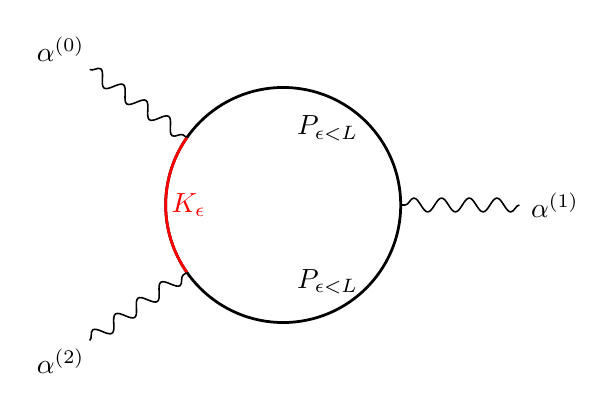
\begin{tikzpicture}[line width=.2mm, scale=1.5]

%\pgfmathsetmacro{\ex}{0}
%\pgfmathsetmacro{\ey}{1}

%\draw (\ex,\ey) ++(45:.8) arc (45:-45:.8);

		\draw[fill=black] (0,0) circle (1cm);
		%\draw[fill=red] (0,0) arc (145:215:1);
		\draw[fill=white] (0,0) circle (0.99cm);
		\draw[line width=0.35mm,red] ++(145:0.995) arc (145:215:0.995);
		%\draw[red] (0,0) arc (30:60:3);

		\draw[vector](145:2) -- (145:1);
		\node at (145:2.3) {$\alpha^{(0)}$};
			%\node at (145:0.85) {$v_0$};
		\node at (60:0.75) {$P_{\epsilon<L}$};
		\node at (-60:0.75) {$P_{\epsilon<L}$};
		\draw[vector](215:2) -- (215:1cm);
		\node at (215:2.3) {$\alpha^{(2)}$};
			%\node at (215:0.85) {$v_{d}$};
		\node[red] at (180:0.8) {$K_\epsilon$};
		\draw[vector](0:2) -- (0:1);
		\node at (0:2.3) {$\alpha^{(1)}$};
			%\node at (35:0.85) {$v_{\alpha}$};
		%\node at (0:0.8) {$P_{\epsilon<L}$};
		%\node at (270:0.8) {$P_{\epsilon<L}$};
	    	\clip (0,0) circle (1cm);
\end{tikzpicture}
\caption{The diagram representing the weight $W_{\Gamma, e}(P_{\epsilon<L}, K_\epsilon, I^\fg)$ in the case $d=2$. 
On the black internal edges are we place the propagator $P_{\epsilon < L}$ of the $\beta\gamma$ system. 
On the red edge labeled by $e$ we place the heat kernel $K_\epsilon$.
The external edges are labeled by elements $\alpha^{(i)} \in \Omega^{0,*}_c(\CC^2)$.}
\label{fig:liewheel}
\end{center}
\end{figure}

In particular, there is no obstruction to having an {\em action} by $\sG$, only an obstruction to having an {\em inner action}. 
Concretely, the external edges of any closed wheel occurring in the expansion of the anomaly must be labeled by $\sG$. 
As an immediate consequence we have the following.

\begin{lem}
The effective family $\{I^{\fg}[L]\}$ defines a one-loop exact $\sG$-equivariant quantum field theory.
In other words, it satisfies the $\sG$-equivariant quantum master equation modulo functionals purely of the background fields $\sG$. 
\end{lem}

It follows that the anomaly $\{\Theta[L]\}$ measures the obstruction to $\{I^\fg[L]\}$ to defining an {\em inner} action. 

%\begin{lem} 
%The one-loop effective family $\{I^\fg[L]\}$ 
%\ben
%I^\fg [L] = \lim_{\epsilon \to 0} W(P_{\epsilon < L}, I^\fg) \mod \hbar^2
%\een
%is well-defined and satisfies the equivariant quantum master equation modulo $\cloc^*(\sG)[[\hbar]]$. 
%\end{lem}
%
%Working modulo $\hbar^2$ Lemma \ref{lem: inner action} implies that the anomaly to $\{I^{\fg}[L]\}$ to satisfying the quantum master equation modulo $\hbar^2$ is an element 
%\ben
%\Theta_V \in \hbar \cloc^*(\sG) .
%\een
%The next subsection is devoted to an explicit calculation of this anomaly using Feynman diagrams. 

\subsubsection{The anomaly calculation}

We now perform the main technical calculation of the anomaly cocycle.

\begin{prop}\label{prop: inner anomaly}
The $L\to 0$ limit of the anomaly cocycle $\Theta = \lim_{L \to 0} \Theta_V[L]  \in \cloc^*(\sG)$ is of the form
\ben
\Theta_V = C \cdot J_{\CC^d}(\ch_{d+1}^\fg (V)),
\een
where $\ch_{d+1}^\fg(V) \in \Sym^{d+1}(\fg^*)^\fg$ and where $J_{\CC^d} : \Sym^{d+1}(\fg^*)^\fg \to \cloc^*(\sG)$ is the map of Lemma \ref{prop j map} and where $C$ some constant only depending on the dimension $d$. 
\end{prop}

To compute the anomaly we refer to the following result about the expression for the anomaly cocycle in terms of the Feynman diagram expansion.
As a direct corollary of our general characterization of chiral anomalies, Lemma \ref{lem: chiral anomaly}, we have the following result.

\begin{lem}\label{lem: g anomaly}
The limit $\Theta_{V} := \lim_{L \to 0} \Theta_{V}[L]$ exists and 
is an element of degree one in $\clie^*(\Vect,\Cloc^*(\fg_n^\CC))$. 
Moreover, it is given by
\ben
\Theta_V = \lim_{\epsilon \to 0} \sum_{\substack{\Gamma \in (d+1)\text{\rm -vertex wheels}\\ e \in {\rm Edge}(\Gamma)}} W_{\Gamma,e}(P_{\epsilon<1}, K_\epsilon,
I^{\rm \fg}[\epsilon]),
\een
where the sum is over wheels $\Gamma$ with $(d+1)$ vertices and a distinguished inner edge $e$.
\end{lem}

%Part of the data of a free theory is a gauge fixing condition $Q^{GF}$. 
%This is an operation on fields of cohomological degree $-1$ and enables us to fix the propagator uniquely. 
%For the $\beta\gamma$ system on $\CC^d$ with values in the vector space $V$ the gauge fixing operator we choose is 
%\ben
%Q^{GF} = \dbar^* \tensor \id_V = \pm \sum_i \frac{\partial}{\partial z_i} \frac{\partial}{\partial (\d \zbar_i)} \tensor \id_V .
%\een

%The propagator with UV-IR cutoff $\epsilon,L$ is equal to
%\ben
%P_{\epsilon, L} (z, w) = \int_{t = \epsilon}^L \dbar^* K_t(z,w)\d t .
%\een
%Here, 
%\ben
%K_t (z,w) = k_t(z,w) \Omega(z,w) (\id_V \tensor 1 + 1 \tensor \id_{V^*})
%\een
%where $k_t$ the heat kernel for the Dolbeault Laplacian $\dbar^* \dbar + \dbar \dbar^*$ acting on smooth functions on $\CC^d$, $\Omega(z,w)$ is a constant coefficient differential form on~$\CC^d_z \times \CC^d_w$ satisfying
%\ben
%\int_{z \in \CC^d} \phi(z) \wedge \Omega(z,w) = \pm \phi(w),
%\een
%and $\id_V , \id_{V^*} \in \Sym^2(V \oplus V^*)$ represent the identity maps $V \to V$, $V^* \to V^*$. 
%Explicitly, if we choose a basis $\{e_a\}$ for $V$ with dual basis $\{e_a^*\}$ we have the following formula for $K_t(z,w)$: 
%\ben
%K_t(z,w) = \frac{1}{(4 \pi t)^d} e^{-|z-w|^2/ t} \left((\d^d z - \d^d w) \wedge \prod_{i} (\d \zbar_i - \d \Bar{w}_i) \right) \left(\sum_{a = 1}^{\dim V} (e_a \tensor e_a^* + e_a^* \tensor e_a) \right).
%\een

%Now, we are ready to apply Lemma \ref{lem anomaly} to compute the anomaly cocycle. 
%The fact that the limit of $W(P_{\epsilon,L}, I^{\sL})$ as $\epsilon \to 0$ exists is technical and left in the appendix. 
%We provide an explicit analysis of the sum of the Feynman weights corresponding to wheels.
%We find that the sum reduces to evaluating the weight of a single wheel with $d+1$ vertices. 

%Fix $k \geq 1$ to be the number of vertices of the wheel $\Gamma$. 
%By differential form type reasons, the wheels with number of vertices $k \leq d$ vanish identically. 
%To see this, note that the integral computing the Feynman weight is an integral over $\CC^{dk}$. 
%Each propagator contributes a differential form of Dolbeault type $(d, d-1)$.
%The heat kernel contributes a differential form of type $(d,d)$. 
%Thus, in total the internal edges contribute a differential form of type 
%\ben
%(kd, (k-1)(d-1) + d) = (kd, (k-1)d + 1).
%\een
%Now, t	he anomaly is a cocycle of $\sL$ of cohomological degree $+1$.
%\brian{finish}
%
%The reason that the wheels of valency $k > d+1$ vanish is more subtle, and relies on analytic bounds of the integral computing the weight. 
%We provide this argument in the appendix. 

The lemma implies that we only need to consider the wheel with $d+1$ vertices. 
Each trivalent vertex is labeled by both an analytic factor and Lie algebraic factor. 
The Lie algebraic part of each vertex can be thought of as the defining map of the representation $\rho : \fg \to {\rm End}(V)$. 
The diagrammitcs of the wheel amounts to taking the trace of the symmetric $(d+1)$st power of this Lie algebra factor. 
Thus, the Lie algebraic factor of the weight of the wheel is the $(d+1)$st component of the character of the representation
\ben
{\rm ch}_{d+1}^\fg(V) = \frac{1}{(d+1)!} {\rm Tr}\left(\rho(X)^{d+1}\right) \in \Sym^{d+1}(\fg^*) .
\een

To finish the calculation we must compute the analytic weight of the wheel with $d+1$ vertices. 
Recall, our goal is to identify the anomaly $\Theta$ with the image of ${\rm ch}_{d+1}^\fg(V)$ under the map
\ben
J : \Sym^{d+1}(\fg^*)^\fg \to \cloc^*(\Omega^{0,*}(\CC^d)\tensor \fg)
\een
that sends an element $\theta$ to the local functional $\int \theta(\alpha \partial \alpha \cdots \partial \alpha)$. 
We have just seen that the Lie algebra factor in local functional representing the anomaly agrees with the $(d+1)$st Chern character. 
Thus, to finish we must show the following.

\begin{lem} 
As a functional on the abelian dg Lie algebra $\Omega^{0,*}(\CC^d)$, the analytic factor of the weight $\lim_{L\to 0} \lim_{\epsilon \to 0} W_{\Gamma, e} (P_{\epsilon < L}, K_\epsilon, I^\fg)$ is equal to a multiple of the local functional
\ben
\int \alpha \partial \alpha \cdots \partial \alpha \in \cloc^*(\Omega^{0,*}(\CC^d)) .
\een
\end{lem}

\begin{proof}

Let's fix some notation. 
We enumerate the vertices by integers $a = 0,\ldots, d$. 
Label the coordinate at the $i$th vertex by $z^{(a)} = (z_1^{(a)}, \ldots, z_d^{(a)})$. 
The incoming edges of the wheel will be denoted by homogeneous Dolbeault forms 
\ben
\alpha^{(a)} = \sum_{J} A^{(a)}_J \d \zbar_J^{(a)} \in \Omega_c^{0,*}(\CC^d) .
\een
where the sum is over the multiindex $J = (j_1,\ldots, j_k)$ where $j_a = 1,\ldots, d$ and $(0,k)$ is the homogenous Dolbeault form type. 
For instance, if $\alpha$ is a $(0,2)$ form we would write
\ben
\alpha = \sum_{j_1 < j_2} A_{(j_1,j_2)} \d \zbar_{j_1} \d\zbar_{j_2} .
\een
Denote the functional obtained as the $\epsilon \to 0$ weight of the wheel with $(d+1)$ vertices from Lemma \ref{lem: g anomaly} by $W_L$.
The $L\to 0$ limit of $W_L$ is the local functional representing the one-loop anomaly $\Theta$. 

The weight has the form
\ben
W_L(\alpha^{(0)},\ldots,\alpha^{(d)}) = \pm \lim_{\epsilon \to 0} \int_{\CC^{d(d+1)}} \left(\alpha^{(0)}(z^{(0)}) \cdots \alpha^{(d)}(z^{(d)}) \right) K_\epsilon(z^{(0)},z^{(d)}) \prod_{a =1}^d P_{\epsilon,L} (z^{(a-1)}, z^{(a)}) .
\een
We introduce coordinates
\begin{align*}
w^{(0)} & = z^{(0)} \\
w^{(a)} & = z^{(a)} - z^{(a-1)} \;\;\; 1 \leq a \leq d .
\end{align*}
The heat kernel and propagator part of the integral is of the form
\[
\begin{array}{ccl}
\displaystyle
K_\epsilon(w^{(0)},w^{(d)}) \prod_{a =1}^d P_{\epsilon,L} (w^{(a-1)}, w^{(a)}) & = & \displaystyle \frac{1}{(4 \pi \epsilon)^d} \int_{t_1,\ldots,t_d = \epsilon}^L \frac{\d t_1 \cdots \d t_d}{(4 \pi t_1)^d \cdots (4 \pi t_d)^d} \frac{1}{t_1\cdots t_d}  \\ & & \displaystyle \times \d^d w^{(0)} \prod_{i=1}^d (\d \Bar{w}^{(1)}_i + \cdots + \d \Bar{w}^{(d)}_i) \prod_{a = 1}^d \d^d w^{(a)} \left(\sum_{i = 1}^d \Bar{w}_i^{(a)} \prod_{j \ne i} \d \Bar{w}_{j}^{(a)}\right)
\\ & & \displaystyle \times e^{-\sum_{a,b = 1}^d M_{a b} w^{(a)} \cdot \Bar{w}^{(b)}} .
\end{array}
\]
Here, $M_{ab}$ is the $d \times d$ square matrix satisfying
\ben
\sum_{a,b = 1}^d M_{a b} w^{(a)} \cdot \Bar{w}^{(b)} = |\sum_{a = 1}^d w^{(a)} |^2 / \epsilon + \sum_{a = 1}^d |w^{(a)}|^2 / t_a .
\een
Note that
\ben
\prod_{i=1}^d (\d \Bar{w}^{(1)}_i + \cdots + \d \Bar{w}^{(d)}_i) \prod_{a = 1}^d \left(\sum_{i = 1}^d \Bar{w}_i^{(a)} \prod_{j \ne i} \d \Bar{w}_{j}^{(a)}\right) = \left( \sum_{i_1,\ldots i_d} \epsilon_{i_1\cdots i_d} \prod_{a=1}^d \Bar{w}^{(a)}_{i_a}\right) \prod_{a=1}^d \d^d \Bar{w}^{(a)} .
\een
In particular, only the $\d w_i^{(0)}$ components of $\alpha^{(0)} \cdots \alpha^{(d)}$ can contribute to the weight.

For some compactly supported function $\Phi$ we can write the weight as
\ben
\begin{array}{ccl}
W (\alpha^{(0)}, \ldots, \alpha^{(d)}) & = & \lim_{\epsilon \to 0} \displaystyle \int_{\CC^{d(d+1)}} \left(\prod_{a = 0}^{d} \d^d w^{(a)} \d^d \Bar{w}^{(a)}\right) \Phi \\ & \times & \displaystyle \frac{1}{(4 \pi \epsilon)^d} \int_{t_1,\ldots,t_d = \epsilon}^L \frac{\d t_1 \cdots \d t_d}{(4 \pi t_1)^d \cdots (4 \pi t_d)^d} \frac{1}{t_1\cdots t_d} \sum_{i_1,\ldots, i_d} \epsilon_{i_1\cdots i_d} \Bar{w}_{i_1}^{(1)} \cdots \Bar{w}_{i_d}^{(d)} e^{-\sum_{a,b = 1}^d M_{a b} w^{(a)} \cdot \Bar{w}^{(b)}} 
\end{array}
\een

Applying Wick's lemma in the variables $w^{(1)}, \ldots, w^{(d)}$, together with some elementary analytic bounds, we find that the weight above becomes to the following integral over $\CC^d$
\ben
f(L) \int_{w^{(0)} \in \CC^d}  \d^d w^{(0)} \d^d \Bar{w}^{(0)} \sum_{i_1,\ldots, i_d} \epsilon_{i_1\cdots i_d}  
\left(\frac{\partial}{\partial w_{i_1}^{(1)}} \cdots \frac{\partial}{\partial w_{i_d}^{(d)}} \Phi\right)|_{w^{(1)}=\cdots=w^{(d)} = 0} 
\een
where
\ben
f(L) = \lim_{\epsilon \to 0} \int_{t_1,\ldots,t_d = \epsilon}^L \frac{\epsilon}{(\epsilon + t_1 + \cdots + t_d)^{d+1}} \d^d t .
\een
In fact, $f(L)$ is independent of $L$ and is equal to some nonzero constant $C \ne 0$.
Finally, plugging in the forms $\alpha^{(0)}, \ldots, \alpha^{(d)}$, we observe that the integral over $w^{(0)} \in \CC^d$ simplifies to
\ben
C \int_{\CC^d} \alpha^{(0)} \partial \alpha^{(1)} \cdots\partial \alpha^{(d)}
\een
as desired.
\end{proof}

This completes the proof of Proposition \ref{prop: inner anomaly}.

\subsection{Local to global}

In this section we finish the proof of our main result Theorem \ref{thm ggrr} by showing how our local calculation above implies the formula for the anomaly on a general compact affine manifold $X$.
By an complex affine manifold, we mean a quotient 
\ben
q : U \subset \CC^d \to X
\een
of an open subset $U \subset \CC^d$ by a free and proper action of a discrete subgroup of the affine group $U(d) \ltimes \CC^d$. 
We consider affine manifolds that are also compact. 
To deduce our main theorem we will show that the theory and the anomaly above also exhibit equivariance for the affine group on $\CC^d$, thus it will descend to any affine manifold.

We have stated the main result for an arbitrary principal $G$-bundle $P$ on the affine manifold $X$. 
Suppose the discrete subgroup $\Gamma \leq U(d) \ltimes \CC^d$ defines the affine manifold $q : U \to X = U / \Gamma$ as above. 
Then, principal $G$-bundles on $X$ are equivalent to $\Gamma$-equivariant principal $G$-bundles on $U$. 

Let $\sE$ be an arbitrary elliptic complex on $X$, and suppose the Lie algebra $\fh$ acts on $\sE$. 
Since $X$ is compact, the cohomology $H^*(\sE(X))$ is finite dimensional.
It therefore makes sense to define the character of the action of $\fh$ on $H^*(\sE(X))$.
\be\label{superchar}
\chi_\sE : \fh \to \CC \;\; , \;\; M \in \fh \mapsto {\rm STr}_{H^*(\sE(X))} (M) .
\ee
Here, STr denotes the supertrace. 
The character factors through the determinant of the representation.
For the graded character above, we must use the superdeterminant which we denote by $\det (H^*(\sE(X)))$. 
Free BV quantization gives a natural field theoretic interpretation of this determinant.

\begin{prop}[\cite{CG2} Lemma 12.7.0.1] 
Let $\sE$ be any elliptic complex on a compact manifold $X$ and let $T^*[-1] \sE$ be the corresponding free BV theory given by the shifted cotangent bundle. 
Let $\Obs^\q_\sE$ be the factorization algebra of quantum observables of this theory.
Then, there is an isomorphism
\ben
H^* \left(\Obs^\q_{\sE}(X) \right) \cong \det H^*(\sE(X)) [n]
\een
where $n$ is the Euler characteristic of $\sE(X)$ modulo $2$. 
\end{prop}

\begin{rmk}
In \cite{GwilliamHaugseng} they prove that an abstracted version of linear BV quantization behaves like a determinant over formal moduli problems.
An immediate consequence is that given a classical theory with an action of a Lie algebra $\fg$, the BV quantization as we consider produces a line bundle over the moduli space $B \fg$. 
Our calculation of the obstruction produces a calculation in terms of Feynman diagrams of the first Chern class of this line bundle. 
\end{rmk}
 
Notice that the classical free theory $\sE_V$ is equivariant for the affine group $U(d) \ltimes \CC^d$.
Thus, it defines a classical theory on any affine manifold $X$.
This theory is free and of the form
\ben
\sE_V (X) = T^*[-1] (\Omega^{0,*}(X , V))
\een
where $T^*[-1]$ denotes the shifted cotangent bundle.
Thus, the global quantum observables satisfy
\be\label{quantum obs}
H^*(\Obs^\q_{V}(X)) = \det \left(H^*(X, \sO^{hol}) \tensor V \right)
\ee
 
%Similarly, the functional $I^\fg$ is equivariant for the affine group, so that it also descents to a functional on $X$.
%Thus, the Noether current $I^\fg$ defines a \brian{finish}

In Section \ref{sec: classical g equiv} we have showed how the classical theory $\sE_{V}$ has an an action by the local Lie algebra $\sG_X$.
This arose from an action of $\sG(X) = \Omega^{0,*}(X, \fg)$ on the elliptic complex $\Omega^{0,*}(X, V)$. 
At the level of cohomology we have an action of $H^*(\sG(X))$ on $H^*(\Omega^{0,*}(X, V))$ and hence a character $\chi_{V}$ as in Equation (\ref{superchar}) which is an element in $H^*_{red}(\sG(X))$. 

The local Lie algebra cohomology of any local Lie algebra embeds inside its ordinary (reduced) Lie algebra cohomology of global sections $\cloc^*(\sL(X)) \subset \cred^*(\sL(X))$. 
The character (\ref{superchar}) is an element in $H_{red}^*(\sL(X))$.
As an immediate corollary of \cite{CG2} Theorem 12.6.0.1 we have the following relationship between the anomaly cocycle and the character.

\begin{prop}\label{inner char}
Suppose $\sL$ is a local Lie algebra that acts on the elliptic complex $\sE$ on a compact manifold $X$.
Let $\Theta_\sE \in \cloc^*(\sL)$ be the local cocycle measuring the failure to satisfy the $\sL$-equivariant classical master equation (that is, the obstruction to having an inner action).
Then, its global cohomology class satisfies $[\Theta_\sE (X)] = \chi_{\sE} \in \cred^*(\sL(X))$ where $\chi_\sE$ is the trace of the action of $H^*(\sL(X))$ on $H^*(\sE(X))$. 
\end{prop}

%\begin{proof}
%A version of this is proved in Section 7 of \cite{GwilliamThesis}, but we will sketch the proof here.
%\end{proof}

For the case of $\sL = \sG_X$ we have an embedding of cochain complexes
\ben
\cloc^*(\sG(X)) \hookrightarrow \cred^*(\sG(X)) = \cred^*(\Omega^{0,*}(X) \tensor \fg) .
\een
By Kodaira-Spencer theory have already seen that the global sections of the local Lie algebra $\sG(X)$ is a model for the formal neighborhood of the trivial $G$-bundle inside of $G$-bundles. 
In particular, the $\sG(X)$-module of quantum observables defines a line bundle $\int_X \Obs^\q_{\sE_V}$ over this formal neighborhood.
Its character as a $\sG(X)$-module is identified with the first Chern class of the corresponding line bundle $\chi_\sE(\Obs^\q_{V}(X)) = c_1(\int_X \Obs^\q_{V})$. 

Now, notice that the one-loop quantization we constructed in the previous section, as well as the anomaly cocycle $\Theta_V \in \cloc^*(\sG_{\CC^d})$ are equivariant for the group $U(d) \ltimes \CC^d$. 
Thus, they descend to the global sections of $\cloc^*(\sG_X)$ for any affine manifold $X$.
Explicitly, if $\Gamma\subset U(d) \ltimes \CC^d$ is the discrete subgroup such that $X = U / \Gamma$ where $U \subset \CC^d$, then under the isomorphism 
\ben
\cloc^*(\sG(X)) \cong \cloc^*(\sG(U))^\Gamma
\een
we have $\Theta_V(X) \leftrightarrow \Theta_V(U)$.

Further, we have an identification
\ben
\cred^*(\Omega^{0,*}(X) \tensor \fg) = \sO_{red}\left({\rm Bun}_G(X)^{\wedge}_{triv}\right) \cong  \Omega^1_{cl} \left({\rm Bun}_G(X)^{\wedge}_{triv}\right) 
\een
where we have used the equivalence of reduced functions and closed one-forms which makes sense on any formal moduli space.
At the level of $H^1$ we have the composition composition
\be\label{cohbung}
\Sym^{d+1}(\fg^*)^\fg \xto{J^X} H^1_{\rm loc} (\sG(X)) \to H^1(\Omega^1_{cl}\left({\rm Bun}_G(X)^{\wedge}_{triv}\right) .
\ee
As a corollary of Proposition \ref{inner char} and our calculation of the local anomaly cocycle we see that the image of $\ch_{d+1}^\fg(V)$ is equal to $[\Theta_V(X)] = [c_1(\int_X \Obs^\q_V)]$. 

The same holds when we work around any holomorphic principal bundle $P$ on $X$, so that we have an embedding of cochain complexes
\ben
\cloc^*(\sAd(P)(X)) \hookrightarrow  \Omega^1_{cl} \left({\rm Bun}_G(X)^{\wedge}_{P}\right) . 
\een
which determines a composition
\be\label{cohbung}
\Sym^{d+1}(\fg^*)^\fg \xto{J_P^X} H^1_{\rm loc} (\sAd(P)(X)) \to H^1(\Omega^1_{cl}\left({\rm Bun}_G(X)^{\wedge}_{P}\right) .
\ee
Since every principal $G$-bundle $P$ on $X$ is trivial when we pull it back to $U\subset \CC^d$, the above local anomaly calculation proves that $[c_1(\int_X \Obs^\q_{P,V})] = C \ch_{d+1}^\fg (V)$ in this case as well.
This completes the proof of Theorem \ref{thm ggrr}. 

\subsection{A module for the higher Kac-Moody}

The last part of this section we diverge to deduce a consequence of the quantum Noether theorem using our analysis above by exhibiting a module for the higher affine algebras from the previous section. 
For convenience, we fix the trivial $\fg$-bundle $P = {\rm triv}$ so that $\sAd(P) = \sG_X$.

On any manifold $X$, the quantum Noether theorem, Theorem 12.1.0.1 of \cite{CG2}, provides a map of factorization algebras
\ben
\Phi_X : \UU_\alpha (\sG_X) \to \Obs^\q_{V} ,
\een
for some $\alpha \in H^1_{\rm loc}(\sG_X)$.
The factorization algebra $\Obs^\q_V$ is the quantum observables of the $\beta\gamma$ system on $X$ with values in the $\fg$-module $V$. 
This is a free field theory, thus the above map has the flavor of a {\em free field realization} of the Kac-Moody factorization algebra.
In particular when $X = \CC^d$, or any affine manifold, the calculation above shows that there is a map of factorization algebras
\ben
\Phi_{\CC^d} : \UU_{\ch_{d+1}(V)} (\sG_{\CC^d}) \to \Obs^\q_{V} .
\een

Next, consider the case $X = \CC^d \setminus  \{0\}$. 
By functoriality of pushforwards, the quantum Noether theorem produces a map of one-dimensional factorization algebras
\ben
\rho_* \Phi : \rho_* \UU_{\ch_{d+1}(V)} (\sG_{\CC^d \setminus \{0\}}) \to \rho_* \Obs^\q_{V} .
\een
We have exhibited a locally constant dense subfactorization algebra $\sF^{lc}_{1d}$ of $\rho_* \UU_\alpha (\sG_X)$ which is equivalent, as an $E_1$-algebra, to $U \Hat{\fg}_{d, \ch_{d+1}(V)}$. 
Similarly, in Section \ref{sec: sphere ops} we have shown that there is a locally constant dense subfactorization algebra that is equivalent to the dg algebra $\sA_V$. 

The map $\rho_* \Phi$ restricts to these dense subfactorization algebras and so defines a map of $E_1$ algebras
\ben
\rho_* \Phi : U \Hat{\fg}_{d, \ch_{d+1}(V)}\to \sA_V .
\een
Also, in Section \ref{sec: disk module} we have shown how the disk operators $\sV_V$ form a module, through the factorization product, for the dg algebra $\sA_V$. 
This is essentially the Fock module of the algebra $\sA_V$, thus we should view the above map $\rho_*\Phi$ as being a higher dimensional analog of the ``free field realization" for the higher dimensional affine algebras. 

Further, by induction along the map $\rho_* \Phi$, we obtain the following.

\begin{prop}
The map $\rho_*\Phi$ endows the space $\sV_V$ with the structure of a module over the $E_1$-algebra $U \Hat{\fg}_{d, \ch_{d+1}(V)}$.
Equivalently, $\sV_V$ is an $A_\infty$-module for $U \Hat{\fg}_{d, \ch_{d+1}(V)}$. 
\end{prop}

The module $\sV_V$ is the prototype for a higher dimensional version of the vacuum Verma module for ordinary affine algebras. 
It is enticing to construct the higher excitation Verma modules as dg modules for the higher affine algebras we've considered in this thesis.
We do not do that here, but hope to return to it in future work.

\section{Holomorphic diffeomorphisms}

The next type of symmetry we consider is that of holomorphic reparametrizations, or holomorphic diffeomorphisms. 
A holomorphic diffeomorphism $f : X \to Y$ between complex manifolds is a bijective holomorphic map whose inverse is also holomorphic.
Under composition, holomorphic diffeomorphisms from $X$ to itself combine to form a Lie group ${\rm Diff}^{hol}(X)$.
We study theories that have an action of holomorphic diffeomorphisms which leave the action functional invariant.
An example of such a theory is one for which the action functional can be written down in a holomorphically covariant way (e.g. one that only uses universal constructions in complex geometry). 
Morally speaking, the Lie algebra of holomorphic diffeomorphisms from $X$ to itself is equal to holomorphic vector fields on $X$.
This may seem obvious, but some care must be taken to make this precise as ${\rm Diff}^{hol}(X)$ is not a finite dimensional manifold.
In \cite{KM97} a formalism for studying infinite dimensional diffeomorphism groups and their Lie algebras is developed, and we refer the reader there for a more in depth discussion of these issues.
We will not be concerned with these functional analytic issues since we will take as a starting point theories that have symmetries by the Lie algebra of holomorphic vector fields. 
It is an interesting question if our constructions lift to the level of the Lie group, but we will not address that here.

\subsection{Holomorphic vector fields}

Covariance in field theory is usually reserved for theories that can be written in a way that uses only natural constructions in differential geometry and so is independent of a choice of a local coordinate. 
This is precisely the condition that the theory is invariant with respect to the group of diffeomorphisms
The obvious holomorphic analog of this makes sense for theories defined on complex manifolds. 
In this section we introduce a local-to-global Lie algebraic version of holomorphic covariance using a natural local Lie algebra associated to holomorphic diffeomorphisms.

In the two-dimensional chiral case we will see that a holomorphic covariant theory is the same thing as a chiral conformal field theory.
In higher dimensions, holomorphically covariant theories arise from natural mathematical situations such as the holomorphic $\sigma$-model we met in the last chapter.

From a physical standpoint, holomorphically covariant theories can be obtained via holomorphic twists of supergravity theories.
In this thesis, we have not addressed what it means to twist a supergravity theory (let alone what supergravity is), but the foundational work has been developed in \cite{CostelloLiSUGRA}. 
In collaboration with Chris Elliott, we will show in a future publication how the twist of the most basic supergravity theory, four-dimensional $\cN = 1$ supergravity, admits a holomorphic twist to a holomorphically covariant theory. 
The relationship of the symmetry by holomorphic vector fields on twists of supergravity theories is one of our main applications for developing the theory in this section.

\subsubsection{The local Lie algebra}

Just as in the case of holomorphic gauge symmetries, there is a local Lie algebra associated to holomorphic vector fields. 
For any complex manifold $X$, the holomorphic tangent bundle $T^{1,0}X$ is a holomorphic vector bundle and hence admits a Dolbeault complex $\Omega^{0,*}(X, T^{1,0}X)$.
Together with the $\dbar$ operator, there is a natural extension of the Lie bracket of holomorphic vector fields that gives this complex the structure of a dg Lie algebra.
The underlying graded vector space of $\Omega^{0,*}(X, T^{1,0}X)$ is clearly the global sections of a smooth graded vector bundle.
Moreover, the differential and Lie bracket are differential and bidifferential operators respectively. 
Thus:

\begin{dfn/lem} 
For any complex manifold $X$, $\Omega^{0,*}(X, T^{1,0}X)$ has the structure of a local Lie algebra that we denote $\sT_X$.
\end{dfn/lem}

In keeping with the conventions above, when we want to stress the sheaf-like nature of this local Lie algebra we use the notation $\sT^{sh}_X$. 
This is a sheaf of dg Lie algebras which assigns to an open set $U \subset X$ the dg Lie algebra $\Omega^{0,*}(U, T^{1,0}U)$. 
We will use the notation $\sT_X$ to denote the associated cosheaf $U \mapsto \Omega^{0,*}_c(U, T^{1,0}U)$.

\subsubsection{Holomorphically covariant theories}

The local Lie algebra $\sT_X$ allows us to define the following stronger notion of a holomorphic theory. 
Recall the definition of a holomorphic theory on a complex manifold $X$ from Section \ref{sec: hol theory}.
This consists of the data of a holomorphic vector bundle $V \to X$, a holomorphic differential operator $Q^{hol} : V \to V[1]$, a shifted symplectic pairing $(-,-)_V$ on $V$, and a holomorphic Lagrangian density $I^{hol}$.

\begin{dfn}
A holomorphic theory $(V, Q^{hol}, \omega, (-,-)_V, I^{hol})$ is {\em holomorphically covariant} if the associated BV theory admits an action by the local Lie algebra $\sT_X$.  
\end{dfn}

Many of the holomorphic theories we have encountered are, in addition, holomorphically covariant. 
Recall that the data of an action of a local Lie algebra $\sL$ on a theory $\sE$ is given by a Maurer-Cartan element in the the dg Lie algebra ${\rm Act}(\sL, \sE)[-1]$ from Section \ref{sec: local equiv}. 
This is a sub dg Lie algebra of $\cred^*(\sL(X)) \tensor \oloc(\sE)[-1]$ where the dependence on the local Lie algebra must also be local.

\begin{eg}
Consider the $\beta\gamma$ system on a complex manifold $X$ with values in a vector space $V$.  
We consider this theory extensively in Section \ref{sec: local obs}.
The fields $\sE_V$ consist of elements $\gamma \in \Omega^{0,*}(X,V)$ together with their conjugates. 
The dg Lie algebra $\sT(X)$ acts on the cochain complex $\Omega^{0,*}(X,V)$ via Lie derivative: if $\xi \in \sT(X)$ of degree $k$ and $\gamma \in \Omega^{0,l}(X)$ then $L_\xi \gamma \in \Omega^{0,k+l}(X, V)$ is defined. 
It is immediate to see that this is compatible with the $\dbar$ operator.
The classical Noether current defining the classical action is
\ben
I^{\sT}(\xi, \beta,\gamma) = \int \<\beta, L_\xi \gamma\>_V ,
\een
where $\<-,-\>$ is, as usual, the pairing between $V$ and its dual.
This functional defines a Maurer-Cartan element in
\ben
I^{\sT} \in {\rm Act}(\sT, \sE_V) [-1] \subset \cred^*(\sT(X)) \tensor \oloc(\sE_V)[-1]
\een
and hence we have a classical action of $\sT_X$ on $\sE_V$. 
\end{eg}

There is a variation of this example that plays an important role for us.
The holomorphic tensor bundle of type $(r,s)$ on a manifold $X$ is the holomorphic vector bundle
\ben
V^s_r = \underbrace{T^{1,0} X \tensor \cdots \tensor T^{1,0} X}_{r \; {\rm copies}} \tensor \underbrace{T^{*1,0}X \tensor \cdots \tensor T^{*1,0}X}_{s \; {\rm copies}} .
\een 
Similarly, there are anti-holomorphic versions.
The local Lie algebra $\sT_X$ acts on any holomorphic tensor bundle on $X$ via Lie derivative.
This extends to a map
\ben
L : \sT_X \times \Omega^{0,*}(X, V_r^s) \to \Omega^{0,*}(X, V_r^s) \; \; , \;\; (\xi, \gamma) \mapsto L_\xi \gamma , 
\een
giving the Dolbeault complex $\Omega^{0,*}(X, V_r^s)$ the structure of a dg module for $\sT(X)$. 
In a completely analogous way to the lemma above, we have the following. 

\begin{lem}
The $\beta\gamma$ system twisted by the tensor bundle of type $(r,s)$ has an action by the local Lie algebra $\sT_X$ given by the local functional
\ben
I^{\sT} (\xi, \gamma, \beta) = \int \<\beta, L_\xi \gamma\>_{V^s_r} .
\een
Hence, it is a holomorphically covariant theory.
\end{lem}

\subsubsection{Higher central charges}

Just as in the case of the current algebra, we can apply the factorization enveloping algebra to $\sT_X$ to obtain a factorization algebra $\UU (\sT_X)$ on any complex manifold $X$. 
The interesting deformations of this factorization algebra come from local cocycles on $\sT_X$ which define the twisted enveloping algebras.

\begin{dfn}
Let $\alpha \in H^1_{loc}(\sT_X)$.
The {\em Virasoro factorization algebra} on $X$ of central charge $\alpha$ is the twisted factorization enveloping algebra $\UU_\alpha(\sT_X)$. 
\end{dfn}

The motivation for the term {\em central charge} will become clear momentarily. 
For a complex manifold of dimension one, we have shown in \cite{BWVir} that $H^*_{loc}(\sT_\Sigma) = \Omega^*(\Sigma) [1]$.
Thus, on a connected Riemann surface there is a unique, up to scale, local cohomology class of degree one that we normalize by $H^1_{loc}(\sT_\Sigma) = \CC \cdot \omega_{Vir}$.
This cocycle $\omega_{Vir}$, which we will recall below, is related to the cocycle defining the usual extension of the one-dimensional Witt algebra.  
Moreover, in \cite{BWVir}, we have shown that locally this twisted factorization envelope recovers the Virasoro vertex algebra.
Implicit in the statement below is the relationship between one-dimensional holomorphic factorization algebras and vertex algebras that we recalled at the beginning of Section \ref{sec: sphere ops}.

\begin{thm}[\cite{BWVir}]
Let $c \in \CC$. 
The factorization envelope $\UU_{c \cdot \omega_{Vir}}(\sT_\CC)$ is a holomorphically translation invariant factorization algebra and its cohomology defines a vertex algebra $\Vert(\UU_{c \cdot \omega_{Vir}}(\sT_\CC))$.
Moreover, this vertex algebra is isomorphic to the Virasoro vertex algebra of charge $c$:
\ben
\Vert(\UU_{c \cdot \omega_{Vir}}(\sT_\CC)) \cong {\rm Vir}_c .
\een
\end{thm}

We will see how this twisted factorization enveloping algebra appears when studying quantization of holomorphically covariant theories in any dimension. 

The definition of a quantum field theory that is holomorphically covariant is similar to the classical case.
We refer again to Section \ref{sec: local equiv} for the definition of an action of a local Lie algebra on a quantum field theory.
Recall, there were essentially two separate notions of a quantum symmetry: that of an action by a local Lie algebra $\sL$, and that of an {\em inner action}. 
To have an action of a local Lie algebra, one must prescribe a family of $\sL$-dependent functionals $\{I^{\sL}[L]\}$ satisfying the renormalized quantum master equation modulo functionals that dependent solely on $\sL$. 
To have an inner action, the quantum master equation must be satisfied on the nose.
We have discussed a deformation theory for lifting an action to an inner action; in particular, there is an obstruction that lives in $H^1_{\rm loc}(\sL)$ to lifting an action to an inner action. 

\begin{dfn}
A quantum field theory is holomorphically covariant if it admits an action by the local Lie algebra $\sT_X$. 
The {\em central charge} of a holomorphically covariant quantum field theory is the obstruction to lift this action to an inner action.
This is an element 
\ben
\fc_\sE \in H^1_{\rm loc}(\sT_X) [[\hbar]] .
\een
\end{dfn}

In complex dimension one, this definition agrees with the usual definition of the central charge in chiral conformal field theory.

\subsubsection{Chiral conformal field theory}\label{sec: chiral cft}

\def\Riem{{\rm Riem}}
\def\Conf{{\rm Conf}}

In complex dimension one there is an intimate relationship between complex structures and Riemannian structures. 
Every Riemann surface admits a natural Riemannian metric and hence a conformal structure. 
Conversely, a conformal class of a metric defines a complex structures. 
It is well-known that the moduli of Riemann surfaces is equivalent to the moduli of conformal structures.

We can see this at the level of local Lie algebras as follows. 
Fix a Riemann surface $\Sigma$ and denote by $g_0$ the associated Riemannian metric. 
Define the {\em Riemannian local Lie algebra} as follows.
Using the fixed metric $g_0$ define the two-term complex
\ben
{\rm Riem}(\Sigma, g_0) = \Gamma(\Sigma, T \Sigma) \xto{L g_0} \Sym^2(T^*\Sigma) [-1]
\een
where the differential sends a vector field $X$ to $L_X g_0$, the Lie derivative of $g_0$ with respect to $X$. 
The Lie bracket of vector fields gives this complex the structure of a dg Lie algebra.
Better yet, it is immediate to see that it is a local Lie algebra.
The dg Lie algebra $\Riem(\Sigma,g_0)$ is the derived replacement for the one-shifted tangent space of the moduli space of Riemannian structures on $\Sigma$ at $g_0$. 

There is a natural map of local Lie algebras $\sT_\Sigma \to \Riem(\Sigma,g_0)$. 
In degree zero this is just the inclusion of the holomorphic tangent bundle inside of the full tangent bundle. 
In degree one, note that the metric $g_0$ defines an inclusion
\ben
T^{*0,1}\Sigma \tensor T^{1,0}\Sigma \cong_{g_0} T^{*0,1}\Sigma \tensor T^{*1,0} \Sigma \subset \Sym^2(T^*\Sigma) .
\een
Elements of degree one are sections of the bundle on the left-hand side.
The map in degree one is the inclusion above.

Next, we define the {\em conformal local Lie algebra}.
This is similar to the Riemannian local Lie algebra where we take into account conformal equivalences of metrics. 
Define the two-term complex
\ben
{\rm Conf}(\Sigma, g_0) = \Gamma(\Sigma, T\Sigma) \oplus C^\infty(\Sigma) \xto{D_{g_0}} \Sym^2(T^*\Sigma) [-1] .
\een
The differential is defined by $D_{g_0}(X, f) = L_X g_0 + f g_0$.
The second term encodes the infinitesimal action of the conformal group. 
The Lie bracket of vector fields combined with the obvious action of vector fields on functions gives the above complex the structure of a local Lie algebra.
Of course, every Riemannian structure defines a conformal structure, so there is a map of local Lie algebras $\Riem(\Sigma, g_0) \to \Conf(\Sigma, g_0)$. 

Thus, we obtain a composition
\be\label{local Lie seq}
\sT_\Sigma \to \Riem(\Sigma, g_0) \to \Conf(\Sigma,g_0) .
\ee
Every conformal field theory (in perturbation theory around the metric $g_0$) is hence a holomorphically covariant theory in our sense. 

For conformal field theories, the Weyl, or trace, anomaly is the quantity that measures the central charge.
At the level of the Lie algebra $\Conf(\Sigma, g_0)$ the Weyl anomaly is represented by the local $1$-cocycle 
\ben
\phi^{g_0}_{\rm Weyl}(X, f, \alpha) = \int_\Sigma f R_{g_0 + \alpha} {\rm dvol}_{g_0 + \alpha} + \int_{\Sigma} {\rm Jac}(X) R_{g_0 + \alpha} {\rm dvol}_{g_0 + \alpha},
\een
where $R_{g_0 + \alpha}$ is the scalar curvature of the metric $g_0 + \alpha$ expanded formally in the variable $\alpha$.
One immediately checks that $\phi_{\rm Weyl}^{g_0} \in \cloc^*(\Conf(\Sigma, g_0))$ is a cocycle of cohomological degree one.
Moreover, under the map of local Lie algebras, one checks that $\phi_{\rm Weyl}^{g_0}$ pulls back to the cocycle $\omega_{\rm Vir} \in \cloc^*(\sT_\Sigma)$ defined by
\ben
\omega_{\rm Vir}(\xi_1, \xi_2 \d \zbar) = \int_\Sigma {\rm Jac}(\xi_1) \partial({\rm Jac}(\xi_2)) \d \zbar
\een
We have already remarked that $\omega_{\rm Vir}$ is the generator of the cohomology $H^1_{\rm loc}(\sT_\Sigma)$ for any Riemann surface.
Thus, in complex dimension one we see that our definition of central charge agrees with the usual one from CFT.
We have verified an explicit calculation of the central charge in the BV formalism for a particular holomorphic theory on Riemann surfaces in \cite{BWVir}.

\subsection{Gelfand-Fuks cohomology} \label{sec: gf}

Our aim is to classify the space of central charges of a holomorphically covariant quantum field theory in any dimension.
The description we give will be in terms of a certain cohomology of vector fields on the disk, called {\em Gelfand-Fuks} cohomology. 
In this section we recall some facts about the Lie algebra cohomology of formal vector fields $\W_d$ on the $d$-disk with values in certain non-trivial modules. 
We refer to Section \ref{sec: gk formal geometry} for the requisite notation for objects living on the formal disk.

In Section \ref{sec: formal atiyah} we have constructed the formal Atiyah class for any formal vector bundle $\cV$ on $\hD^n$. 
It is an element of the relative Gelfand-Fuks cohomology
\ben
\At^{\GF}(\cV) \in \clie^1(\W_d,\GL_d; \hOmega^1_d \otimes_{\hO_d} \End_{\hO_d}(\cV)) .
\een
From the Atiyah class we have built the formal Chern character using the usual formula 
\ben
\ch^{\GF}(\cV) = \Tr\left(\exp\left(\frac{1}{2\pi i} \At^{\GF}(\cV)\right)\right),
\een
and have studied how components of this formal Chern character give rise to $L_\infty$ extensions of $\W_d$ that appear as natural universal symmetries of quantizations of higher dimensional holomorphic $\sigma$ models with target $\hD^d$. 

In this section we arrive at the Lie algebra of formal vector fields, and its cohomology, from a different perspective. 
Instead of using formal geometry to construct universal objects on the {\em target} of a $\sigma$ model, we will see how Gelfand-Fuks classes characterize holomorphic symmetries on the higher {\em world-sheet}, or source manifold. 

The symmetry is that of holomorphic reparametrizations. 
Infinitesimally, this is described by the Lie algebra of holomorphic vector fields. 
Classical theories on a complex manifold $X$ with such a symmetry by holomorphic reparametrizations admit an action by the local Lie algebra $\sT_X = \Omega^{0,*}(X , T_X^{1,0})$. 

The Gelfand-Fuks classes we will consider in this section appear as anomalies for quantizing an action by the local Lie algebra $\sT_X$. 
In other words, these classes parametrize shifted central extensions of $\sT_X$, just as the classes $\theta \in \Sym^{d+1}(\fg^*)^\fg$ defined central extensions of the current algebra $\fg^X$. 
By our usual yoga of studying equivariant quantizations, we know such anomalies live in the local cohomology complex $\cloc^*(\sT_X)$. 


\begin{dfn/lem} Consider the following two classes of cocycles on $\W_d$.
\begin{itemize}
\item[Chern type:] For $1 \leq k \leq d$, let $\tau_k \in \clie^k(\W_d ; \hOmega_d^k)$ be the cocycle
\ben
\tau_k = s_k \left(\At^{\GF}(\hT_d)\right),
\een
where $s_k(\At^{\GF}(\hT_d)) $ is the homogeneous degree $k$ piece of the characteristic polynomial defined by $\det(I + t \At^{\GF}(\hT_d))$. 
\item[$\GL$ type:] For $1 \leq i \leq d$ let $a_i \in \clie^{2i-1}(\W_d ; \hO_d)$ be the cocycle 
\ben
a_i : (\xi_1,\ldots,\xi_{2i-1}) \mapsto \sum_{\sigma \in S_{2i-1}} {\rm sign}(\sigma) \Tr({\rm Jac}(\xi_{\sigma(1)}) \cdots {\rm Jac}(\xi_{\sigma(2i-1)}) .
\een
\end{itemize}
\end{dfn/lem}

We will use the notation $\hOmega_d^\# = \oplus_{k} \hOmega^k_d [-k]$ to denote the graded $\W_d$-module with $\hOmega^k_d$ sitting in degree $k$. 
The wedge product of forms endows this $\W_d$-module with the structure of a graded commutative algebra. 

If $V$ is a graded vector space then we use the notation $\CC[V]$ to denote the free graded $\CC$-algebra on $V$.
If $V$ is spanned by vectors $\{v_i\}$ we will use the shorthand $\CC[v_i]$ for this graded algebra. 

\begin{thm}[\cite{GFnontrivial}] \label{thm nontrivial coeff} The bigraded commutative algebra $H^*(\W_d ; \hOmega_d^{\#})$ is isomorphic to the bigraded commutative algebra 
\ben
\left. \left(\CC[a_1,\ldots, a_{2d-1}, \tau_1,\ldots,\tau_d]\right) \right/ \left(\tau_1^{j_1}\cdots \tau_d^{j_d} \right),
\een
where the quotient is over all indices $\{j_1,\ldots,j_d\}$ that satisfiy $j_1 + 2j_2 + \cdots + d j_d > d$. 
Here $a_{2i-1}$ is in bidegree $(2i-1,0)$ and $\tau_j$ is in bidegree $(j,j)$. 
\end{thm}

In the above result we have not turned on the de Rham differential $\d_{dR} : \hOmega^k_d \to \hOmega_d^{k+1}$. 
This endows $\hOmega^*_d = (\hOmega^\#_d, \d_{dR})$ with the structure of a dg commutative algebra in $\W_d$-modules. 
The formal Poincar\'{e} lemma asserts that the inclusion of the trivial $\W_d$-module 
\ben
\CC \xto{\simeq} \hOmega^*_d
\een 
is a quasi-isomorphism. 
In turn, we obtain a quasi-isomorphism of Chevalley-Eilenberg complexes
\ben
\clie^*(\W_d) \xto{\simeq} \clie^*(\W_d ; \hOmega_d^*) . 
\een 
We may think of the cochain complex $\clie^*(\W_d ; \hOmega_d^*)$ as the total complex of the double complex with vertical differential given by the $\W_d$ Chevalley-Eilenberg differential for the graded module $\hOmega_d^\#$, and horizontal differential equal to the de Rham differential. 

To any double complex there is a spectral sequence abutting to the cohomology of the total complex. 
The $E_1$ page of this spectral sequence is given by the cohomology of the vertical differential. 
Moreover, if the double complex is a bigraded algebra so are each of the pages. 
In this case, the $E_1$ page is precisely the bigraded algebra of Theorem \ref{thm nontrivial coeff} and we have a spectral sequence
\be\label{ss1}
E^{p,q}_2 = \left(H^q(\W_d ; \hOmega^p_d), \d_{dR}\right) \implies H^*(\W_d ; \hOmega^*_d) \cong H^*(\W_d) .
\ee

\begin{eg}
For the case $d = 1$ the spectral sequence collapses at the $E_2$ page. 
The only nontrivial cohomology is $\CC$ in bidegree $(0,0)$ and $a_1 \cdot \tau_1$ in bidgree $(1,2)$. 
The $1$-cocycle valued in formal power series $a_1$ is given by $a_1(f_i \partial_i) = \partial_i f_i \in \hO_n$. 
The $1$-cocycle valued in formal $1$-forms $\tau_1$ is given by $\tau_1(g_j \partial_j) = \d_{dR}(\partial_j g_j)$. 
To obtain the generator of $H^3({\rm W}_1)$ we perform the following zig-zag:
\ben
\xymatrix{
\clie^3({\rm W}_1) \ar[r] & \clie^3({\rm W}_1 ; \hO_1) & \\
& \clie^2({\rm W}_1 ; \hO_1) \ar[u]^-{\d_{CE}} \ar[r]^-{\d_{dR}} & \clie^2({\rm W}_1; \hOmega^1_1) . 
} 
\een
The de Rham differential kills $a_1 \cdot \tau_1$, so there exists an $\alpha \in \clie^2({\rm W}_1 ; \hO_1)$ such that $\d_{dR} \alpha = - a_1 \cdot \tau_1$. 
Now, the class $\d^{\hO}_{CE} \alpha \in \clie^3({\rm W}_1 ; \hO_n)$ satisfies
\begin{align*}
\d_{dR} (\d^{\hO}_{CE} \alpha) & = - \d_{CE} (a_1 \tau_1) = 0 \\
\d_{CE} \d_{CE}^{\hO} \alpha & = 0 .
\end{align*}
Here, $\d_{CE}^{\hO}$ denote the Chevalley-Eilenberg differential for $\clie^*(\W_1 ; \hO_1)$ and $\d_{CE}$ is the restriction of this Chevalley-Eilenberg differential to $\clie^*(\W_1)$. 
The first line says that $\d_{CE}\alpha$ lifts to $\clie^3(\W_1)$, and the second line says that it is a cocycle for the absolute cohomology.  
Finally, note that $(\d_{CE}^{\hO} + \d_{dR} ) \alpha = \d_{CE}^{\hO} \alpha - a_1 \tau_1$. 
Thus, in the total complex $\d_{CE}^{\hO} \alpha$ is homotopic to $a_1 \tau_1$, and so $[\d_{CE}^{\hO} \alpha]$ is the generator of $H^3(\W_1)$. 
\end{eg}

For general $d \geq 1$, one can apply this spectral sequence to understand the cohomology $H^*(\W_d)$. 
To describe it, we introduce the following topological space. 
Let ${\rm Gr}(d,n)$ be the complex Grassmannian of $d$-planes in $\CC^n$. 
Denote by ${\rm Gr}(d,\infty)$ the colimit of the natural sequence 
\ben
{\rm Gr}(d,d) \to {\rm Gr}(d, d+1) \to \cdots . 
\een 
It is a standard fact that ${\rm Gr}(d, \infty)$ is a model for the classifying space $B\U(d)$ of principal $\U(d)$-bundles. 
Let $E\U(d) \to B\U(d)$ be the universal principal $\U(d)$-bundle. 
Using the colimit description above, we have a natural skeletal filtration of $B\U(d)$ by 
\ben
{\rm sk}_{k} B\U(d) = {\rm Gr}(d, k) .
\een 
Let $X_d$ denote the restriction of $E\U(d)$ over the $2d$-skeleton:
\ben
\xymatrix{
X_d \ar[r] \ar[d] & E \U(d) \ar[d] \\
{\rm sk}_{2d} B \U(d) \ar[r] & B\U(d) .
}
\een

\begin{rmk}
Though not the way the Gelfand and Fuks originally proved the result, one can use the computation of the cohomology of $\W_d$ with coefficients in $\hOmega^k_d$ together with the spectral sequence (\ref{ss1}) to prove this description of $H^*(\W_d)$. 
Indeed, the spectral sequence (\ref{ss1}) is isomorphic, up to regradings, to the Serre spectral sequence for the principal $\U(d)$-bundle $X_d \to {\rm sk}_{2d} B \U(d)$. 
In other words, the formal de Rham differential on $\hOmega^*_d$ is exactly the $E_2$ differential for the Serre spectral sequence. 
\end{rmk}

\begin{thm}[\cite{Fuks} Theorem 2.2.4] 
There is an isomorphism of graded vector spaces
\ben
H^*(\W_d) \cong H^*_{dR} (X_d) .
\een
Moreover, the commutative algebra structure on $H^*(\W_d)$ is trivial. 
\end{thm}

Note that when $d = 1$ we have ${\rm sk}_2 B \U(1) = \PP^1 \subset \PP^\infty = B \U(1)$. 
Moreover, the restriction of the universal bundle is Hopf fibration $U(1) \to S^3 \to \PP^1$. 
In particular, one has $X_1 = S^3$.
An immediate application of the Serre spectral sequence shows that first nontrivial cohomology above degree zero of $X_d$ is in degree $(2d+1)$ and is identified with $H^{2d+2}(B \U(d))$ for any dimension $d$. 
Thus, $H^{2d+1}(\W_d) = H^{2d+2}(B\U(d))$. 


\subsection{The local cohomology of holomorphic vector fields}

Our main result in this section is a complete classification of the local cohomology of the sheaf of Dolbeualt complex of holomorphic vector fields $\sT_X = \Omega^{0,*}(X ; T_X^{1,0})$ on any complex manifold.
This description involves the Gelfand-Fuks cohomology of formal vector fields that we have just discussed and will give a classifications of the higher dimensional central charges for holomorphically covariant field theories.

The proof relies heavily on our construction of Gelfand-Kazhdan descent from Chapter \ref{chap: holsig}. 
The key difference, is that the formal geometry utilized in this section is on the {\em source} rather than the target as we used it in the previous chapter. 

\begin{thm}
Let $X$ be a complex $d$-fold. 
There is a quasi-isomorphism of sheaves of cochain complexes
\ben
\cloc^*(\sT_X) \; \simeq \; \Omega^*_X \tensor \cred^*(\W_d) [2d] 
\een
where $\Omega^{*}_X$ is the sheaf of de Rham forms on $X$. 
\end{thm}

The core of the argument is in interpretting the local Lie algebra cohomology as the cohomology of vector fields on the formal disk through the process of {\em Gelfand-Kazhdan descent} that we introduced in Chapter \ref{chap: holsig}.
Before moving on to the proof, we have the immediate cohomological interpretation of the calculation.
Recall that when we study classical BV theories equivariant for a local Lie algebra $\sL$, the space the failure for quantizing the BV theory in a way that is equivariant for the Lie algebra is measured by an anomaly class in the local cohomology.
For holomorphic diffeomorphisms, we obtain the following. 

\begin{cor} 
For $X$ any complex manifold of complex dimension $d$ one has at the level of cohomology 
\ben
H^k_{\rm loc}(\sT_X) \; \cong \; \bigoplus_{i=0}^{2d} H^i_{dR}(X) \tensor H^{2d + k-i}_{\rm Lie, red}(\W_d) .
\een
In particular, if the manifold is connected the space of anomalies for holomorphic diffeomorphisms for a theory defined on $X$ is:
\ben
H^{1}_{\rm loc}(\sT_X) =  H^{2d+1}_{\rm Lie}(\W_d)  ,
\een
which is independent of the complex manifold.
\end{cor}

Applying the isomorphism $H^{2d+1}(\W_d) = H^{2d+2}(BU(d))$, we see that the local cocycles of holomorphic vector fields come from universal characteristic classes in $d$-dimensions. 
There is a geometric explanation for this akin to the case of the moduli of $G$-bundles in the previous section.
Let $\sM$ be the moduli space of complex manifolds of dimension $d$.
A rigorous mathematical definition of this object as a derived stack has not appeared in the detail that \cite{FHK} give for $G$-bundles, but we will only use it as a motivating object. 
Over the moduli space there is the universal complex $d$-fold $\pi : \sX \to \sM$ whose fiber over $[X] \in \sM$ is $X$ itself. 
Any tensor bundle $\sV$ (those built from the tangent bundle via duals and tensor products) defines a vector bundle over $\sX$. 
Further, this vector bundle defines a locally free sheaf of $\sM$ via the derived pushforward $\RR \pi_* \sV$ and hence a Chern class $c_1(\sV) = c_1(\RR \pi_* \sV) \in H^2(\sM)$. 
These are higher dimensional analogs of the tautological classes on the moduli space of curves.

There is a relationship of these tautological classes with Gelfand-Fuks cohomology as follows. The vector bundle $\sV \to \sX$ is classified by a map $f_{\sV} : \sX \to B \U(d)$, and so we obtain the diagram. 
\ben
\begin{tikzcd}
& \sV \arrow[d] & \\
& \sX \ar[dr,"\pi"] \ar[dl, "f_\sV"'] & \\
B \U(d) & & \sM .
\end{tikzcd}
\een
If $\alpha \in H^{2d+2} (B \U(d))$ we obtain the class via the push-pull construction $\pi_* f_{\sV}^* \alpha \in H^2(\sM)$.
Since $H^{2d+2} (B \U(d)) \cong H^{2d+1}(\W_d)$, this shows that our Gelfand-Fuks classes define tautological classes on the moduli of complex manifolds. 
It would be interesting to work out the precise relationship between the classes $c_1(\sV)$ and Gelfand-Fuks classes, but we postpone this to future work.

%\begin{thm}
%Let $X$ be a complex $d$-fold. 
%There is a quasi-isomorphism of sheaves
%\ben
%J^{GF} : \ul{\clie^*(\W_d ; \hOmega^*_n)}_X [2d] \to \cloc^*(\sT_X)
%\een
%where $\ul{(-)}_X$ denotes the constant sheaf on $X$. 
%Further, by the formal Hodge to de Rham spectral sequence there is a quasi-isomorphism $\ul{\clie^*(\W_d)}_X [2d] \simeq \cloc^*(\sT_X)$ of sheaves on $X$.
%\end{thm}

The corollary implies that the cohomology $H^{2d+1}_{\rm Lie}(\W_d)$ deserves to be thought of as the space of ``higher dimensional central charges" of a classically holomorphic diffeomorphism invariant theory. 
After the proof of our main result we will how this relates to the central extensions of holomorphic vector fields and the role of these extensions in quantum field theory.

\begin{proof}
We recall a description of the local cohomology complex using $D$-modules given in Section 4.5 of \cite{CG2}.
Let $\sL$ be any local Lie algebra on $X$ with associated graded vector bundle $L$.
The local Lie algebra cohomology is defined as the sheaf
\ben
\cloc^*(\sL) = \Omega^{d,d}_X \tensor_{D_X} \cred^*(JL)
\een
where $JL$ is the $D_X$-module given by taking the $\infty$-jets of the underlying vector bundle of $\sL$. 
In \cite{CostelloRenormalization} it was shown that $\cred^*(JL)$ is flat as a $D_X$-module, thus we can replace the tensor product above by a left-derived tensor product
\be\label{derived tensor1}
\Omega^{d,d}_X \tensor_{D_X} \cred^*(JL) \simeq \Omega^{d,d}_X \tensor^{\LL}_{D_X} \cred^*(JL) .
\ee
The Spenser resolution is a free resolution of $\Omega^{d,d}_X$ as a right $D_X$-module (by $D_X$ we mean smooth differential operators) given by
\ben
M^* = \left(\cdots \to \Omega^{2d-1} \tensor_{C^\infty_X} D_X \xto{\nabla_D} \Omega^{d,d} \tensor_{C^\infty_X} D_X\right)
\een
The differential $\nabla_D$ is determined by the natural flat connection on $D_X$.
This complex $M^*$ is concentrated in degree $-2d,\ldots,0$. 
Via this resolution, we see that (\ref{derived tensor1}) is quasi-isomorphic to 
\ben
M^* \tensor_{D_X} \cred^*(JL) \simeq  \left(\cdots \to \Omega^{2d-1} \tensor_{C^\infty_X} \cred^*(JL)  \xto{\nabla_D} \Omega^{d,d} \tensor_{C^\infty_X}\cred^*(JL) \right) .
\een
The right-hand side is, by definition, the shifted de Rham complex of the $D_X$-module $\cred^*(JL)$ so we obtain

\be\label{de rham 1}
\cloc^*(\sL) \simeq \Omega^*(X , \cred^*(JL))[2d] .
\ee

Now, suppose that $\sL$ is a holomorphic local Lie algebra of the form $\Omega^{0,*}(X, L^{hol})$ where $L^{hol}$ is a holomorphic vector bundle. 
In the above notation, the underlying smooth vector bundle is $L = \Wedge^* T^{0,1^*}X \tensor L^{hol}$. 

%We have used the notation $JE$ to denote the smooth sections of the infinite rank vector bundle ${\rm Jet}(E)$. 
%If $E$ is a holomorphic vector bundle let ${\rm Jet}^{hol}(E)$ denote the infinite rank holomorphic vector bundle of holomorphic jets. 
%Similarly, let $J^{hol}E$ be the holomorphic sections of this bundle. 
%This is a $D^{hol}_X$-module where $D^{hol}_X$ is the sheaf of holomorphic differential operators. 
%Equivalently, a $D^{hol}_X$-module is a holomorphic vector bundle with a holomorphic flat connection.
%Of course, any $D_X^{hol}$-module $E$ forgets to a smooth $D_X$-module that we denote $E^{C^\infty}$. 

%Suppose $V$ is a $D_X^{hol}$-module, and consider its holomorphic de Rham complex $\Omega^{*,hol}(X, V)$. 
%Moreover, $V$ forgets down to a $D_X$-module that we denote $V^{C^\infty}$ and we can consider its $C^\infty$ de Rham complex $\Omega^*(X, V^{C^\infty})$. 
%These two de Rham complexes are quasi-isomorphic since they are resolutions of the same sheaf. 

%\begin{lem} \label{lem: hol dmodule}
%There is a quasi-isomorphism of de Rham complexes
%\ben
%\Omega^*(X, E^
%\end{lem}
%\begin{proof}
%Let $\sL$ be the sheaf of sections of $L$. 
%The Dolbeualt complex is a resolution of the sheaf of holomorphic sections; thus there is a quasi-isomorphism $\sL \simeq \sL^{hol}$ of $\sO_X$-modules. 
%\end{proof}

%This means that we can further reduce the expression for the local cohomology in (\ref{de rham 1}) to 
%\be\label{de rham 2}
%\cloc^*(\sL) \simeq \Omega^*(X , \cred^*(J^{hol}L^{hol}))[2d] .
%\ee
%We have dropped the notation $(-)^{C^\infty}$ for convenience.

We now turn to the local Lie algebra in question, namely $\sT_X$. 
This is the local Lie algebra defined by Dolbeualt complex of the holomorphic tangent bundle $T^{1,0}X$, $\sT_X = \Omega^{0,*}(X, T^{1,0}X)$.
As sheaves, of course, there is a quasi-isomorphism $\sT_X \simeq \Gamma^{hol}_X(T^{1,0}X)$ where the right-hand side is the sheaf of holomorphic sections of the holomorphic tangent bundle. 
Similarly, there is a quasi-isomorphism of $D_X$-modules $J \sT_X \simeq J^{hol} T^{1,0}X$.
In particular, there is a quasi-isomorphism of de Rham complexes
\ben
\Omega^*(X , \cred^*(J(\sT_X))) \simeq \Omega^*(X, \cred^*(J^{hol} T^{1,0} X)) .
\een
On the right-hand side note that we take {\em holomorphic} jets.

Suppose now that $\sV$ is any $(\W_d, \GL_d)$-module.
Then, Gelfand-Kazhdan descent along the complex manifold $X$ yields the $D_X$-module $\desc_X(\sV)$. 
In the case that $\sV = \hT_d$ we have seen that the $D_X$-module $\desc_X(\hT_d)$ is equivalent to the $D_X$-module $J^{hol} T^{1,0}X$. 

\begin{lem}
Gelfand-Kazhdan descent is symmetric monoidal. 
That is, if $\sV,\sV'$ are two $(\W_d, \GL_d)$-modules, then
\ben
\sV \tensor_{\hO_n} \sV' \simeq \desc_X(\sV) \tensor_{J^{hol} \sO^{hol}_X} \desc_X(\sV') .
\een
\end{lem}

This implies that there is a string of isomorphisms of $D_X$-modules
\ben
J^{hol} \cred^*(T^{1,0} X) = \desc(\cred^*(\W_d)) \cong \cred^*(\desc(\W_d)) = \cred^*(J ^{hol} T^{1,0} X).
\een
Alternatively, by Proposition A.2 of \cite{GG3} we know that the functor of jets is symmetric monoidal, so the same result follows.

To summarize we see that the Gelfand-Kazhdan descent of the $(\Vect, \GL_d)$-module $\cred(\W_d)$ is equal to the $D_X$-module $\cred^*(J ^{hol} T^{1,0}_X)$.
This is precisely the $D_X$-module present in the definition of the local cohomology of $\sT_X$.
Indeed, we have the quasi-isomorphism
\ben
\cloc^*(\sT_X) \simeq \Omega^*\left(X ,  \cred^*(J^{hol}T^{1,0}_X)\right) .
\een
Thus, the de Rham complex of the $D_X$-module given by descent is precisely the local cohomology 
\ben
\cloc^*(\sT_X) \simeq \Omega^*\left(X , \desc_X(\cred^*(\W_d))\right)
\een

The interpretation via descent will allow us to describe this de Rham complex explicitly. 
Suppose that $\fg$ is any Lie algebra.
Then $\fg$ acts on itself (and its dual) via the adjoint action. 
This extends to an action of $\fg$ on its Chevalley-Eilenberg complex $\clie^*(\fg ; M)$, where $M$ is any $\fg$-module via the formula
\ben
(x \cdot \varphi) (x_1,\ldots, x_k) = \sum_i \varphi(x_1,\ldots, [x, x_i], \ldots,x_k) - x \cdot \varphi(x_1,\ldots,x_k)
\een
Here, $x, x_i \in \fg$ and $\varphi$ is a $k$-cochain with values in $M$.
The $[-,-]$ denotes adjoint action, and the $\cdot$ is the $\fg$-module structure on $M$. 
The following lemma is well-known.
The same formula holds for the reduced cochains.

\begin{lem}
The $\fg$-module structure on the cochain complexes $\clie^*(\fg)$ and $\cred^*(\fg)$ is homotopically trivial.
\end{lem}

For the case of an infinite dimensional Lie algebra, such as $\W_d$, the same result holds when we use the continuous, or Gelfand-Fuks, Lie algebra cohomology.
Thus, $\W_d$ acts homotopically trivial on $\cred^*(\W_d)$.

This implies that the descent $\desc_X(\W_d)$ has a homotopically trivial $D_X$-module structure. 
Equivalently, this means that the flat connection on $\cred^*(J^{hol}T^{1,0}X)$ is gauge equivalent to the trivial connection.
Thus, there is a quasi-isomorphism of de Rham complexes
\ben
\Omega^*\left(X ,  \cred^*(J^{hol}T^{1,0}_X)\right) \simeq \Omega^*(X) \tensor_{C^\infty_X}\ul{\cred^*(\W_d)}_X
\een
where the underline denotes the sections of the trivial bundle with fiber $\cred^*(\W_d)$.
We have identified the left hand side with the local cohomology complex, so we are done.
\end{proof}

\subsection{An explicit description of the local cocycles}

We'd like to leverage our knowledge of the the Gelfand-Fuks cohomology of formal vector fields to provide an explicit description of local cocycles of $\sT_X$. 
The theorem in the previous section gives a very general equivalence of the local cohomology on any complex manifold with the Gelfand-Fuks cohomology, but writing down the form of the local cocycle from the description on a formal disk is not so obvious.

We start with the familiar case $d=1$ and we work on $X = \CC$. 
The cohomology $H^*_{\rm Lie, red}(\W_1)$ is one-dimensional concentrated in degree $3$. 
We'd like to describe the local cocycle corresponding to the generator of $H^3(\W_1) \cong H^1_{\rm loc}(\sT_{\CC})$ explicitly. 
Recall, using the formal Hodge-to-de Rham spectral sequence we saw that the generator of $H^3(\W_1)$ came from the element $a_1 \tau_1 \in H^2_{\rm Lie} (\W_1 ; \hOmega^1_1)$ on the $E_2$ page of the spectral sequence (\ref{ss1}). 

Now, the $1$-cocycles $a_1,\tau_1$ can both be interpreted as functionals on the Dolbeault complex $\Omega^{0,*}(\CC, T^{1,0}\CC)$. 
Indeed, if $\xi = \alpha(z,\zbar) \partial_z$ is an element of the Dolbeault complex we can define
\begin{align*}
\Tilde{a}_1 (\xi) & = \partial_z \alpha(z,\zbar) \in \Omega^{0,*}(\CC) \\
\Tilde{\tau}_1 (\xi) & = \partial (\partial_z \alpha(z,\zbar)) \in \Omega^{1,*}(\CC) .
\end{align*}
Each of these cocycles clearly only depends on the jet of the vector field $\alpha \partial_z$.
Similarly, the product is $\Tilde{a}_1 \Tilde{\tau}_1$ is the bilinear functional on jets of $\sT_\CC$:
\begin{align*}
\Tilde{a}_1 \Tilde{\tau}_1 (\xi_1,\xi_2) & = \partial_z \alpha_1(z,\zbar)  \partial (\partial_z \alpha_2(z,\zbar)) \in \Omega^{1,*}(\CC)
\end{align*}
This is a density precisely when $|\alpha_1|+|\alpha_2| = 1$.
Thus, $\Tilde{a}_1 \Tilde{\tau}_1$ determines a degree $+1$ density valued cochain on $J \sT_\CC$; in other other words an element of $\cloc^*(\sT_\CC)$ that we write as
\ben
\int_\CC \partial_z \alpha_1(z,\zbar)  \partial (\partial_z \alpha_2(z,\zbar)),
\een
which is the local cocycle we denoted $\omega_{Vir}$ above.
If we integrate by parts, we can put this local functional in the form $\int f \partial^3_z g \d z \d \zbar$.
If one restricts this local functional to the annulus and performs the radial integration, we recover the usual formula for the generator of $H^2({\rm Vect}(S^1))$, see \cite{BWVir}, defining the central extension of the Virasoro Lie algebra.

%\ben
%\left(f(z,\zbar) \frac{\partial}{\partial z}, g(z,\zbar)\d \zbar \frac{\partial}{\partial z} \right) \mapsto \int_\CC \left(\frac{\partial}{\partial z} f \right) \partial \left(\frac{\partial}{\partial z} g\right) \d \zbar .
%\een

%For instance, the linear functional $\tau_1 : g(t) \frac{\partial}{\partial t} \mapsto \d_{dR} (\partial_t g(t))$ is mapped to the functional on the Dolbeualt complex of holomorphic vector fields given by $g(z,\zbar) \frac{\partial}{\partial z} \mapsto \partial (\partial_z g(z,\zbar))$. 

\subsubsection{From GF classes to local functionals}

%The description of the one-dimensional local cocycle above be generalized to arbitrary dimensions in a natural way. 
%From a Gelfand-Fuks class in $\clie^*(\W_d ; \hOmega^d_d)$, we will construct a local functional on the local Lie algebra $\sT_{\CC^d}$.
%Suppose $\varphi \in \cred^k (\W_d ; \hOmega^p_d)$ is closed for the Chevalley-Eilenberg differential. 
%We view $\varphi$ as a symmetric linear map
%\ben
%\varphi : \W_d^{\tensor k} \to \hOmega^{p}_d .
%\een
%By closedness for the Lie algebra differential, this is a map of modules for the Harish-Chandra pair $(\W_d, \GL_d)$ and hence for any complex manifold $X$ it determines a map of holomorphic jet bundles
%\ben
%{\rm desc}_X(\varphi) : {\rm Jet}^{hol} (T_X^{1,0})^{\tensor k} \to {\rm Jet}^{hol}(\hOmega^{d,0}_X).
%\een
%This is the descent functor applied to the map $\varphi$. 
%We have used the fact that descent is symmetric monoidal.
%We can further project onto the the zero jet component to obtain a map of bundles
%\ben
%\varphi^X : ({\rm Jet}^{hol} (T_X^{1,0}))^{\tensor k} \to \Omega^{p,0}_X .
%\een
%Since $\varphi^X$ is a map of holomorphic vector bundles, it determines a map on the associated Dolbeault complexes:
%\ben
%\varphi^X : ({\rm Jet} (\sT_X))^{\tensor k} \to \Omega^{p,*}_X.
%\een
%If $\omega \in \Omega^{d-p,*}_X$ is a differential form of type $(d-p,*)$ we obtain a composition
%\ben
%({\rm Jet} (\sT_X))^{\tensor k} \xto{\varphi^X} \Omega^{p,*}_X \xto{\wedge \omega} \Omega^{d,*}_X \to \Omega^{d,d}_X .
%\een 
%In the last map we have projected onto the density component of a differential form.
%Thus, from the Gelfand-Fuks class $\varphi$ we have produced a density valued functional on jets of the local Lie algebra $\sT_X$. 
%This is precisely a local functional on $\sT_X$.
%
%Thus, we have a map
%\ben
%\Omega^*_X \tensor \cred^*(\W_d ; \hOmega^*_d) \to \Omega^{d,d}_X \tensor \cred^*(J \sT_X)
%\een
%which induces the quasi-isomorphism $\Omega^*_X \tensor \cred^*(\W_d) [2d] \simeq \cloc^*(\sT_X)$ that we established above.

The description of the one-dimensional local cocycle above be generalized to arbitrary dimensions in a natural way. 
From a Gelfand-Fuks cocycle $\varphi \in H^k(\W_d ; \hOmega^d_d)$, we will construct a local functional on the local Lie algebra $\sT_{\CC^d}$.
We take a representative for $\varphi$ and view it as a symmetric linear map
\ben
\varphi : \W_d^{\tensor k} \to \hOmega^d_d .
\een
By Corollary 2.2.5 in Chapter 3 of \cite{Fuks} they show that any cohomology class on $\W_d$ with values in any tensor module can be represented by a cocycle which depends only on the $2$-jets of its inputs. 
Thus, up to an exact cocycle, we can assume that $\varphi$ is of the form
\ben
\varphi(X_1,\ldots,X_k) = \sum_{I = (i_1,\ldots,i_k)} D_{i_1} (X_1) \cdots D_{i_k}(X_k) \d^d t
\een
where $D_{i_j} : \W_d \to \hO_d$ are order two differential operators. 

Choosing a coordinate $\{z_i\}$ on $\CC^d$ these operators define holomorphic differential operators
\ben
D_{i_j} : \Gamma^{hol}(\CC^d ; T^{1,0} \CC^d) \to \sO^{hol} ,
\een
and hence extend to differential operators on the compactly supported Dolbeualt complex
\ben
D_{i_j} : \sT_{\CC^d} \to \Omega^{0,*}_c(\CC^d) .
\een

Thus, we see that $\varphi$ defines a symmetric linear map
\ben
\varphi : \sT_{\CC^d} ^{\tensor k} \to \Omega^{d,*}_c(\CC^d) .
\een
In other words, for a collection of compactly supported Dolbeault valued sections of the holomorphic tangent bundle $\xi_1,\ldots,\xi_k$ we obtain a compactly supported $(d,*)$-form $\varphi(\xi_1,\ldots,\xi_k)$. 
In turn, we can integrate this to get a number.
We denote the resulting cochain by
\ben
K_\varphi : \sT_{\CC^d} ^{\tensor k} \to \CC \;\; , \;\; (\xi_1,\ldots,\xi_k) \mapsto \int_{\CC^d} \varphi(\xi_1,\ldots,\xi_k) .
\een

\begin{lem}
For any $\varphi$ the cochain $K_\varphi$ is a local cochain, that is $K_\varphi \in \cloc^*(\sT_{\CC^d})$. 
\end{lem} 

%Notice that we have made no claim about the closedness of the cochain $K_\varphi$. 
%We conjecture that $K_\varphi$ is closed if and only if the class $\varphi \in H^{k}(\W_d ; \hOmega^{d}_n)$ is closed for the $E_2$-differential ...\brian{finish}

For degree reasons, each of the classes in $H^{d+1}(\W_d ; \hOmega^{d}_d)$ survive to the $E_\infty$-page of the formal Hodge-to-de Rham spectral sequence converging to $H^*(\W_d)$, though there may be relations among them. 
We expect, though have not thoroughly checked, that for such  the classes $K_\varphi$ are cocycles in the local Chevalley-Eilenberg complex. 
In dimension two, this is the case.

\begin{eg}
Consider the case $d=2$. 
Using the formal Hodge-to-de Rham spectral sequence, we can choose generators of $H_{\rm Lie}^5(\W_2) = \CC^2$ defined by the classes
\ben
a_1\tau_1^2, a_1 \ch^{\GF}_2 \in H_{\rm Lie}^3(\W_2 ; \hOmega^2_2) .
\een
Where $\ch_2^{\GF} = \frac{1}{2} (\tau_1^2 - 2 \tau_2)$. 
Following the prescription above, the local functionals associated to these cocycles read
\ben
K_{a_1 \tau_1^2}(\xi_1,\xi_2,\xi_3) = \int_{\CC^2} \Tr(\Jac(\xi_1)) \wedge \Tr(\partial \Jac(\xi_2)) \wedge \Tr(\partial \Jac (\xi_3)) .
\een
and
\ben
K_{a_1 \ch_2^{\GF}} (\xi_1,\xi_2,\xi_3) = \int_{\CC^2} \Tr(\Jac(\xi_1)) \wedge \Tr(\partial \Jac(\xi_2) \wedge \partial \Jac (\xi_3)).
\een
It is a direct calculation to show that both $K_{a_1 \tau_1^2}, K_{a_1 \tau_2}$ are local cocycles.
\end{eg}
%We have seen that the cochain complex $\clie^*(\W_d ; \hOmega_d^*)$, equipped with the total differential $\d_{CE} + \d_{dR}$, computes the absolute Gelfand-Fuks cohomology $H^*(\W_d)$ through the formal Hodge to de Rham spectral sequence.
%We will use this property to represent elements of $H^*(\W_d)$ by local functionals on $\sT_X$ by first representing elements in $\clie^*(\Vect ; \hOmega^*_d)$ by local functionals.
%
%We can decompose an element $\alpha \in \clie^k(\W_d ; \hOmega^*_d)$ as 
%\ben
%\alpha = f^I \d t_I .
%\een
%The sum is over the multi-index $I = (i_1,\ldots, i_k)$, where $1 \leq i_j \leq d$.
%For each $I$, $f^I$ is a $k$ multi-linear symmetric functional on $\W_d$ valued in $\hO_d$
%\ben
%f^I : \Sym^k(\W_d [1]) \to \hO_d .
%\een 
%We extend $f^I$ to a functional on the Dolbeault complex $\Omega^{0,*}(\CC^d ; T^{1,0} \CC^d)$ as follows. 
%Using the framing on $\CC^d$, every element of the Dolbeualt complex can be written as
%\ben
%X^{J} (z,\zbar) \d \zbar_J
%\een
%where $J = (j_1,\ldots, j_l)$ is a multi-index and $X^J$ is an ordinary holomorphic vector field on $\CC^d$.
%We extend $f^I$ to a Dolbeualt valued functional $\Omega^{0,*}(\CC^d ; T^{1,0}\CC^d)$ via the formula
%\ben
%\begin{array}{cccc}
%f^I_{\Omega^{0,*}} : & \Sym^k\left(\Omega^{0,*}(\CC^d ; T^{1,0})\right) & \to & \Omega^{0,*}(\CC^d) \\ 
%&\left(X_1^{J(1)} (z,\zbar) \d \zbar_{J(1)}, \ldots, X^{J(k)}_k (z,\zbar) \d \zbar_{J(k)} \right) & \mapsto & f^I(X_1^{J(1)} , \ldots, X^{J(k)}_k) \d \zbar_{J(1)} \wedge \cdots \d \zbar_{J(k)} 
%\end{array}
%\een
%
%The local functional corresponding to the original element $\alpha = f^I \d t_I \in \clie^*(\Vect ; \hOmega^*_d)$ is defined by the $k$-multi-linear functional
%\ben
%(\xi_1, \ldots, \xi_k) \mapsto \int_{\CC^d} f^I_{\Omega^{0,*}}(\xi_1,\ldots, \xi_k) \d z_I .
%\een
%Denote this functional by $J^{GF}(\alpha)$. 
%Note that it is only nonzero when the multi-index $I$ is a permutation of $(1,\ldots, d)$. 
%Since it is given by the integral of a some multi-differential operators against a density it is manifestly a local functional. 


%\begin{lem}
%Let $\cloc^*(\sT_{\CC^d})$ be the local functionals of $\sT_{\CC^d}$ on $\CC^d$. The map
%\ben
%J^{GF} : \clie^*(\W_d ; \hOmega^*_n)[2d] \to \cloc^*(\sT_{\CC^d}) 
%\een
%sending $\alpha \mapsto J^{GF}(\alpha)$ is a map of cochain complexes. 
%\end{lem}
%
%\begin{proof}
%It suffices to show that the map 
%\end{proof}

%\begin{lem}
%Let $\cloc^*(\sT_{\CC^d})^{\CC^d}$ denote the translation invariant local cochain complex of the local Lie algebra $\sT_{\CC^d}$.
%Then, there is a quasi-isomorphism
%\ben
%\clie^*(\W_d)[2d] \xto{\simeq} \cloc^*(\sT_{\CC^d})^{\CC^d} .
%\een
%\end{lem}
%\begin{proof}
%By Lemma \ref{??} we know that if $\sL = \Gamma(L)$ is any holomorphically translation invariant local Lie algebra on $\CC^d$ then there is a quasi-isomorphism
%\ben
%\cloc^*(\sL)^{\CC^d} \simeq \CC \cdot \d^d z \tensor^{\LL}_{\CC[\partial_1,\ldots,\partial_d]} \clie^*(J_0L) [d]
%\een
%where $J_0L$ denotes the $\infty$-jets of $L$ at $0 \in\CC^d$. 
%There is a Koszul resolution of the trivial right $\CC[\partial_1,\ldots,\partial_d] = \CC\left[\frac{\partial}{\partial z_1},\ldots, \frac{\partial}{\partial z_d}\right]$ given by
%\ben
%\left(\CC\left[\frac{\partial}{\partial z_1},\ldots, \frac{\partial}{\partial z_d}\right] [\epsilon_1,\ldots,\epsilon_d], \d \epsilon_i = \frac{\partial}{\partial z_i} \right)
%\een
%where $\epsilon_i$ put in cohomological degree $-1$. 
%Thus, we can write
%\ben
%\cloc^*(\sL)^{\CC^d} \simeq \clie^*(J_0L) [d]
%\een
%\end{proof}

\begin{rmk}
It is an interesting, and subtle, problem to write down the explicit formula for a global representative of the local cocycle corresponding to a Gelfand-Fuks class in $H^{2d+1}(\W_d)$. 
The primary issue is that the formula for the cocycle on $\CC^d$, which we defined above, depends on the choice of a coordinate.
When $d=1$ we show how the choice of a projective connection on a Riemann surface allows one to ``correct" the naive expression for the local cocycle to one that is coordinate independent and hence glues to define a global cocycle.
Moreover, any two projective connections define the same cohomology class associated to the local cocycle.
Such constructions have also appeared in the physics literature related to the ``diffeomorphism anomaly" in conformal field theory \cite{Lazz}. 
In future work we aim to classify the geometric structure on a general complex $d$-fold needed to correct the naive local cocycle to one that glues across the global manifold. 
\end{rmk}


\subsubsection{A comparison to other cocycles}

We have already seen in Section \ref{sec: chiral cft} that when $d=1$ the unique local cocycle associated to the generator in $H^3(\W_1)$ agrees with the Weyl anomaly in CFT. 
There has been an extensive effort in both the physics and math community to classify cocycles pertaining to conformal anomalies in any dimension. 
In real dimensions 4 and 6 see \cite{Bonora, KMM} and for conjectures in higher dimensions see \cite{DeserSchwimmer}. 
Our results above classify holomorphic versions of these conformal anomalies in arbitrary even dimensions. 

In complex dimensions 2 and 3 the dimension of the space of the degree one local cohomology $H^1_{\rm loc}(\sT_X)$ agrees with dimension of the space of non-equivalent cocycles for the higher conformal anomalies studied in \cite{Bonora, DeserSchwimmer}. 
Specifically, in complex dimension $2$ (so real dimension $4$) this space is $2$-dimensional corresponding to the characteristic classes $c_1^3, c_1c_2 \in H^6(BU(2))$. 
In complex dimension $3$ this space is $4$-dimensional corresponding to the classes $c_1^4, c_1^2c_2, c_1c_3, c_2^2$. 
It would be interesting to directly relate our local cocycles to theirs. 

These references describe two classes of cocycles: Type a and type b-cocycles.
In any dimension, there is a single type a-cocycle, and the remaining cocycles are of type b.
Using the isomorphism $H^{2d+1}(\W_d) \cong H^{2d+2}(BU(d))$ we conjecture that the type $a$-cocycle corresponds to the characteristic class $c_1c_{d} \in H^{2d+2}(BU(d))$.

%\subsection{The holomorphic anomaly for $\sigma$-models}

\end{document}